%*******************************************************
%  Teoria de Redes de Petri Hierárquica de Sinais
%  Eugênio Simão – UFSC, Araranguá, 2026
%  Estilo: ClassicThesis (A. Miede) – adaptação PT-BR
%*******************************************************
\documentclass[
    twoside, openright, titlepage,
    numbers=noenddot,
    headinclude, footinclude,
    cleardoublepage=empty,
    paper=a4, fontsize=11pt
]{scrreprt}

%— configuração principal (ver classicthesis-config-pt.tex)
%*******************************************************
%  classicthesis-config-pt.tex
%  Configuração ClassicThesis adaptada para português (PT-BR)
%  Baseada no classicthesis-config.tex de André Miede
%*******************************************************

% ── Cores (deve vir antes de tikz ou qualquer pacote que carregue xcolor) ───
\PassOptionsToPackage{dvipsnames,svgnames,x11names}{xcolor}
\usepackage{xcolor}

% ── Codificação ──────────────────────────────────────────────
\PassOptionsToPackage{utf8}{inputenc}
  \usepackage{inputenc}
\PassOptionsToPackage{T1}{fontenc}
  \usepackage{fontenc}

% ── ClassicThesis (Palatino) ─────────────────────────────────
\PassOptionsToPackage{
  drafting=false,
  tocaligned=false,
  dottedtoc=false,
  eulerchapternumbers=false,
  floatperchapter=true,
  eulermath=false,
  beramono=false,
  palatino=true,
  style=classicthesis
}{classicthesis}

% ── Identificação do documento ───────────────────────────────
\newcommand{\myTitle}{Teoria de Redes de Petri Hierárquica de Sinais\xspace}
\newcommand{\mySubtitle}{Um Arcabouço Formal para Controle Regulatório
  Multi-Escala em Sistemas Celulares\xspace}
\newcommand{\myDegree}{Professor Titular\xspace}
\newcommand{\myName}{Eugênio Simão\xspace}
\newcommand{\myUni}{Universidade Federal de Santa Catarina\xspace}
\newcommand{\myFaculty}{Departamento de Engenharia de Computação\xspace}
\newcommand{\myDepartment}{Campus Araranguá\xspace}
\newcommand{\myLocation}{Araranguá, Santa Catarina\xspace}
\newcommand{\myTime}{Novembro de 2025\xspace}

% ── Abreviaturas ─────────────────────────────────────────────
\providecommand{\ie}{i.\,e.}
\providecommand{\Ie}{I.\,e.}
\providecommand{\eg}{e.\,g.}
\providecommand{\Eg}{E.\,g.}
\newcommand{\cf}{cf.\xspace}

% ── Idioma ───────────────────────────────────────────────────
\PassOptionsToPackage{brazil,english}{babel}
  \usepackage{babel}
\usepackage{csquotes}

% ── Matematica ───────────────────────────────────────────────
\PassOptionsToPackage{fleqn}{amsmath}
  \usepackage{amsmath}
\usepackage{mathtools}   % estende amsmath: dcases, \mathclap, \shortintertext
\usepackage{amssymb}
\usepackage{amsfonts}
\usepackage{amsthm}

% ── Gráficos ─────────────────────────────────────────────────
\usepackage{graphicx}
\usepackage{float}          % [H] placement specifier
\usepackage{scrhack}
\usepackage{xspace}

% ── Tabelas ──────────────────────────────────────────────────
\usepackage{tabularx}
  \setlength{\extrarowheight}{3pt}
\usepackage{booktabs}
\usepackage{longtable}
\usepackage{array}
\usepackage{multirow}
\newcommand{\tableheadline}[1]{\multicolumn{1}{l}{\spacedlowsmallcaps{#1}}}
\newcommand{\myfloatalign}{\centering}
\usepackage{subfig}
\usepackage{wrapfig}        % text-wrapped figures

% ── Algoritmos ───────────────────────────────────────────────
\usepackage{algorithm}
\usepackage{algpseudocode}

% ── Química ──────────────────────────────────────────────────
\usepackage[version=4]{mhchem}

% ── TikZ (Redes de Petri) ────────────────────────────────────
\usepackage{tikz}
\usetikzlibrary{arrows.meta, positioning, petri, shapes, calc}

% ── Símbolos (pifont para \ding, etc.) ───────────────────────
\usepackage{pifont}

% ── Bibliografia (biblatex/biber) ─────────────────────────────
\PassOptionsToPackage{%
  backend=biber,
  citestyle=abnt,
  bibstyle=numeric,
  sorting=nyt,
  natbib=true,
  hyperref=true
}{biblatex}
\usepackage{biblatex}

% ── Referência à última página (ficha catalográfica) ────────
\usepackage{lastpage}

% ── Microtype ────────────────────────────────────────────────
\usepackage{microtype}

% ── Ambientes matemáticos ────────────────────────────────────
\theoremstyle{definition}
\newtheorem{definition}{Definição}[chapter]
\newtheorem{principle}[definition]{Princípio}
\newtheorem{example}[definition]{Exemplo}
\theoremstyle{plain}
\newtheorem{theorem}[definition]{Teorema}
\newtheorem{lemma}[definition]{Lema}
\newtheorem{corollary}[definition]{Corolário}
\newtheorem{proposition}[definition]{Proposição}
\theoremstyle{remark}
\newtheorem{remark}[definition]{Observação}

% ── Símbolo QED ──────────────────────────────────────────────
\renewcommand{\qedsymbol}{$\blacksquare$}

% ── Operadores matemáticos (predicados do formalismo SHPN) ───
% Usados nas provas formais; \DeclareMathOperator produz espaçamento correto
\DeclareMathOperator{\Enabled}{Enabled}
\DeclareMathOperator{\Fire}{Fire}
\DeclareMathOperator{\NEnabled}{NormalEnabled}
\DeclareMathOperator{\TEnabled}{TestEnabled}
\DeclareMathOperator{\SEnabled}{SignalEnabled}
\DeclareMathOperator{\Preemption}{PreemptionCheck}

% ── Notação de pré/pós-conjunto (Redes de Petri) ─────────────
% Pré-conjunto normal:        \npre{t}  →  {}^\bullet t
\newcommand{\npre}[1]{{}^\bullet{#1}}
% Pós-conjunto normal:        \npost{t} →  t^\bullet
\newcommand{\npost}[1]{{#1}^\bullet}
% Pré-conjunto de sinal:      \sigpre{t} → {}^\bullet_s t
\newcommand{\sigpre}[1]{{}^\bullet_s{#1}}
% Pós-conjunto de sinal:      \sigpost{t} → t^\bullet_s
\newcommand{\sigpost}[1]{{#1}^\bullet_s}

% ── Notação de alcançabilidade e semântica de compromisso ─────
% Conjunto de alcançabilidade:   \Reach{M_0}  →  \mathcal{R}(M_0)
\newcommand{\Reach}[1]{\mathcal{R}(#1)}
% Espaço de estados:             \StateSpace  →  \mathcal{M}
\newcommand{\StateSpace}{\mathcal{M}}
% Marcação de compromisso:       \Mcommit{p}  →  M_{\mathrm{commit}}(p)
\newcommand{\Mcommit}[1]{M_{\mathrm{commit}}(#1)}
% Passo de disparo:              \firestep{M}{t}{M'}  →  M \xrightarrow{t} M'
\newcommand{\firestep}[3]{#1 \xrightarrow{#2} #3}
% Alcançabilidade multi-passo:   \reaches{M}{M'}     →  M \xrightarrow{*} M'
\newcommand{\reaches}[2]{#1 \xrightarrow{*} #2}

% ── Espaçamento entre parágrafos (≈ novos blocos de ideia) ───
\setlength{\parskip}{3pt plus 1pt minus 0pt}

% ── Pacote classicthesis ─────────────────────────────────────
\PassOptionsToPackage{hyperfootnotes=false}{hyperref}
\usepackage{classicthesis}

% ── Legenda de figuras/tabelas: alinhamento à extensão (sem recuo) ───────────
\captionsetup{format=plain, justification=justified}

% ── Hyperref ─────────────────────────────────────────────────
\hypersetup{%
  colorlinks=true, linktocpage=true,
  pdfstartpage=3, pdfstartview=FitV,
  breaklinks=true, pageanchor=true,
  pdfpagemode=UseNone,
  plainpages=false, bookmarksnumbered,
  bookmarksopen=true, bookmarksopenlevel=1,
  hypertexnames=true, pdfhighlight=/O,
  urlcolor=CTurl, linkcolor=CTlink, citecolor=CTcitation,
  pdftitle={\myTitle},
  pdfauthor={\textcopyright\ \myName, \myUni},
  pdfsubject={Tese de Concurso para Professor Titular – UFSC},
  pdfkeywords={Redes de Petri, Biologia de Sistemas, Hierarquia de Sinais,
               Bacillus subtilis, UFSC},
  pdfcreator={pdfLaTeX},
  pdfproducer={LaTeX com hyperref e classicthesis}
}

% ── Autoref em português ──────────────────────────────────────
\makeatletter
\@ifpackageloaded{babel}{%
  \addto\extrasbrazil{%
    \renewcommand*{\figureautorefname}{Figura}%
    \renewcommand*{\tableautorefname}{Tabela}%
    \renewcommand*{\partautorefname}{Parte}%
    \renewcommand*{\chapterautorefname}{Capítulo}%
    \renewcommand*{\sectionautorefname}{Seção}%
    \renewcommand*{\subsectionautorefname}{Seção}%
    \renewcommand*{\subsubsectionautorefname}{Seção}%
    \renewcommand*{\equationautorefname}{Eq.}%
  }%
}{\relax}
\makeatother


%— base de referências
\addbibresource{referencias.bib}

%— hifenação extra
\hyphenation{sis-te-mas bio-ló-gi-cos Pe-tri hi-e-rár-qui-co}

%*******************************************************
\begin{document}
\frenchspacing
\raggedbottom
\selectlanguage{brazil}
\pagenumbering{roman}
\pagestyle{plain}

%*******************************************************
%  Frontmatter
%*******************************************************
\begingroup
\thispagestyle{empty}
\begin{center}
  \vspace*{2cm}

  {\scshape\Large Eugenio Simão}\par
  \vspace{0.5cm}
  {\small eugenio.simao@ufsc.br}\par

  \vspace{2cm}

  {\spacedallcaps{\myTitle}}\par
  \vspace{0.6cm}
  {\large\textit{\mySubtitle}}\par

  \vspace{3.5cm}

  %
\includegraphics[width=0.28\textwidth]{vertical_sigla_PB_fundo_claro.png}\par % logo UFSC não versionado

  \vfill

  {\normalsize\myLocation\\ \myTime}\par
  \vspace{2cm}
\end{center}
\endgroup

% ─── Folha de Rosto (página 2) ───────────────────────────────
\begingroup
\thispagestyle{empty}
\begin{center}
  \vspace*{2cm}

  {\scshape\Large \myName}\par
  \vspace{3cm}

  {\spacedallcaps{\myTitle}}\par
  \vspace{0.6cm}
  {\large\textit{\mySubtitle}}\par

  \vspace*{\fill}

  \begin{flushright}
    \begin{minipage}{0.55\textwidth}
      \small
      Tese submetida ao
      \myFaculty\ da \myUni\ --- \myDepartment, como requisito parcial
      para a obtenção do título de \textbf{\myDegree}, na área de
      Bioinformática e Modelagem Computacional.
    \end{minipage}
  \end{flushright}

  \vspace*{\fill}

  {\normalsize\myLocation\\ \myTime}\par
  \vspace{2cm}
\end{center}
\endgroup

\cleardoublepage% ─── Ficha Catalográfica (página 3) ─────────────────────────
\begingroup
\thispagestyle{empty}
\vspace*{\fill}
\begin{center}
  \fbox{%
    \begin{minipage}[c][8cm]{12cm}
      \vspace{0.5cm}
      \noindent
      \textbf{Simão, Eugênio}

      \smallskip
      \noindent
      \myTitle\ : \mySubtitle\ /
      Eugênio Simão --- \myLocation, \myTime.

      \smallskip
      \noindent
      \pageref{LastPage} p. : il. ; 30 cm.

      \smallskip
      \noindent
      Tese ---
      \myUni, \myFaculty, \myDepartment.

      \smallskip
      \noindent
      Inclui referências bibliográficas.

      \smallskip
      \noindent
      1. Redes de Petri Hierárquicas de Sinais.
      2. Biologia de Sistemas Computacional.
      3. Modelagem Formal de Vias Bioquímicas.
      4. Controle Regulatório Multi-Escala.
      I. Título.

      \vspace{0.5cm}
      \noindent
      \textit{(Ficha catalográfica gerada pela Biblioteca Universitária da \myUni.)}
    \end{minipage}
  }
\end{center}
\vspace*{\fill}
\endgroup

\cleardoublepage% ─── Folha de Aprovação (página 4) ──────────────────────────
\begingroup
\thispagestyle{empty}
\begin{center}
  \vspace*{1cm}

  {\scshape\Large \myName}\par
  \vspace{1.5cm}

  {\spacedallcaps{\myTitle}}\par
  \vspace{0.4cm}
  {\large\textit{\mySubtitle}}\par
  \vspace{1.5cm}

  \noindent
  A presente tese foi avaliada e aprovada em concurso público para
  o cargo de Professor Titular do \myFaculty\ da \myUni\ ---
  \myDepartment, pela banca examinadora composta pelos seguintes membros:\par
  \vspace{1.5cm}
\end{center}

\noindent
\rule{0.45\textwidth}{0.4pt}\hfill\rule{0.45\textwidth}{0.4pt}\\[2pt]
{\small Prof.(a)\ [nome], Dr.(a)}\hfill{\small Prof.(a)\ [nome], Dr.(a)}\\
{\small [Instituição]}\hfill{\small [Instituição]}

\vspace{1.2cm}

\noindent
\rule{0.45\textwidth}{0.4pt}\hfill\rule{0.45\textwidth}{0.4pt}\\[2pt]
{\small Prof.(a)\ [nome], Dr.(a)}\hfill{\small Prof.(a)\ [nome], Dr.(a)}\\
{\small [Instituição]}\hfill{\small [Instituição]}

\vspace{1.2cm}

\noindent
\begin{center}
\rule{0.45\textwidth}{0.4pt}\\[2pt]
{\small Prof.(a)\ [nome], Dr.(a)}\\
{\small [Instituição]}
\end{center}

\vspace{1.5cm}

\noindent
Certificamos que esta é a versão original e final do trabalho que foi
julgado adequado para obtenção do título de \textbf{\myDegree}.

\vspace{2cm}

\begin{center}
  \myLocation, \myTime.

  \vspace{2cm}

  \rule{8cm}{0.4pt}\\[4pt]
  {\small Chefe do \myFaculty\ --- \myUni}
\end{center}
\endgroup

\cleardoublepage% ─── Dedicatória (página 5) ──────────────────────────────────
\begingroup
\thispagestyle{empty}
\vspace*{\fill}
\begin{flushright}
  \textit{Aos que trabalham na fronteira entre a matemática e a biologia,\\
  e àqueles que ousam construir pontes entre os dois mundos.}
\end{flushright}
\vspace*{\fill}
\endgroup

\cleardoublepage\pdfbookmark[1]{Agradecimentos}{agradecimentos}
\chapter*{Agradecimentos}

Agradeço à banca examinadora pelas invaluáveis contribuições avaliativas
e ao Departamento de Engenharia de Computação da UFSC pelo suporte
institucional ao longo deste trabalho.

Agradeço igualmente aos colegas da UFSC pelo ambiente intelectual
estimulante, e aos colaboradores cujas perspectivas aprimoraram este
trabalho em vários estágios de seu desenvolvimento.

O desenvolvimento da plataforma SHYpn não teria sido possível sem
o ecossistema de código aberto sobre o qual foi construída. Registro
gratidão especial às comunidades dos projetos Python, NumPy, SciPy e
GTK, cujas contribuições coletivas tornaram viável a implementação.

Agradeço também aos curadores dos bancos de dados KEGG, BRENDA e
ChEBI por manterem os recursos de dados públicos que fundamentam a
integração de parâmetros biológicos neste trabalho; aos estudantes de
pós-graduação que utilizaram versões iniciais da plataforma e
proporcionaram retroalimentação prática; e à minha família pelo apoio
inabalável ao longo desta jornada.

Esta pesquisa recebeu apoio de \textbf{[Agência de Fomento/Número do Processo]}.
Os financiadores não tiveram papel no desenho do estudo, na coleta e análise
dos dados, na decisão de publicar, nem na preparação do manuscrito.

\vspace{2em}
\noindent Simão Eugênio, UFSC, Janeiro de 2026.

\cleardoublepage% ─── Epígrafe ────────────────────────────────────────────────
\begingroup
\thispagestyle{empty}
\vspace*{\fill}
\begin{flushright}
  \textit{``A matemática é a linguagem com a qual Deus escreveu o Universo.''}\\[1em]
  Galileu Galilei
\end{flushright}
\vspace*{\fill}
\endgroup

\cleardoublepage\pdfbookmark[1]{Resumo}{resumo}
\chapter*{Resumo}

Sistemas biológicos exibem organização multi-escala onde vias metabólicas
executam transformações bioquímicas enquanto redes regulatórias controlam a
ativação dessas vias. As abordagens computacionais existentes modelam essas
escalas separadamente, impedindo a predição de limiares de decisão ---
fronteiras quantitativas onde células transitam irreversivelmente entre
fenótipos. Este trabalho apresenta a Teoria das Redes de Petri Hierárquicas de
Sinais, uma extensão formal das Redes de Petri clássicas que possibilita
a modelagem unificada de metabolismo e regulação mediante semântica
composicional.

O formalismo estende a 5-tupla clássica $(P, T, F, W, M_0)$ a uma 13-tupla
que incorpora quatro inovações essenciais.
Os \emph{lugares de sinal} ($\Psi \subset P$) particionam os metabólitos entre
aqueles que executam transferência de massa e os que intermediam controle
regulatório, permitindo que moléculas como o ATP participem simultaneamente da
glicólise (por arcos normais) e do controle do desenvolvimento (por arcos de
fluxo de sinal).
Os \emph{arcos de fluxo de sinal} ($F_s$) implementam transformação de
informação com estequiometria, criando estados regulatórios em cascata através
das camadas hierárquicas.
As \emph{funções de camada hierárquicas}
($\lambda: \Psi \to \mathbb{N}$) atribuem níveis organizacionais com regras de
precedência que garantem que camadas inferiores (metabolismo) preemptam camadas
superiores (regulação gênica).
O \emph{parâmetro termodinâmico} $\Gamma = (K, n, \varepsilon)$ determina
analiticamente o limiar efetivo de habilitação por arco
$\theta_{\text{eff}} = K \cdot (\varepsilon / (1 - \varepsilon))^{1/n}$;
o ponto de comprometimento sistêmico --- a concentração e o instante em que a
rede se compromete irreversivelmente --- emerge da dinâmica acoplada da rede
em lugar de ser ajustado como parâmetro.

A validação do formalismo por meio da esporulação de \emph{Bacillus subtilis},
bem caracterizada na literatura de biologia de sistemas, demonstra capacidade
preditiva quantitativa. A construção de um modelo com 40~lugares e
36~transições a partir de cinéticas enzimáticas publicadas (banco de dados BRENDA)
e estequiometria de fosforretransmissão (literatura bioquímica) reproduziu a
assimetria experimental de \textcite{Fujita2005}: a acumulação gradual de
Spo0A${\sim}$P via fosforretransmissão natural produz esporulação em
${\approx}\,52\%$ das réplicas, enquanto a indução constitutiva abrupta de
Spo0A* (Spo0A-Sad67) produz apenas ${\approx}\,5\%$ --- a separatriz de
comprometimento emerge quando $\sigma^H$ ultrapassa $\theta_{\sigma H}
\approx 1{,}60\,\mu$M (varredura fatorial $2 \times 3 \times 4$, 25~condições,
1250~simulações estocásticas) --- sem ajuste de qualquer parâmetro ao
resultado experimental.
A simulação gerou todas as 16~espécies regulatórias e estruturais da cascata
de esporulação, incluindo esporo maduro, com perfis de concentração e
temporização biologicamente plausíveis.

O formalismo aborda limitações da biologia de sistemas computacional além da
decisão bacteriana. Dinâmicas heterogêneas --- cinética enzimática contínua,
expressão gênica estocástica, pontos de verificação temporais --- executam-se
dentro de uma semântica unificada. A arquitetura regulatória torna-se
topologicamente explícita por meio dos tipos de arco, em vez de implícita nas
equações. A construção automatizada de modelos integra bancos de dados de vias
(KEGG) e enzimas (BRENDA), reduzindo o esforço manual e preservando a exatidão
formal mediante verificação de equilíbrio elementar.

Metodologicamente, as Redes de Petri Hierárquicas de Sinais estabelecem que
semânticas composicionais formais podem abranger escalas organizacionais,
possibilitando uma biologia de sistemas integrada onde limiares de
decisão celular emergem da arquitetura da rede.

\vspace{1cm}
\noindent\textbf{Palavras-chave:} Redes de Petri Hierárquicas de Sinais.
Vias Bioquímicas. Redes de Regulação Gênica. Redes de Petri Bio-Híbridas.
Biologia de Sistemas. Biologia Sintética. Modelagem \textit{in~silico}.

\cleardoublepage

% ── Abstract (inglês) ────────────────────────────────────────
\pdfbookmark[1]{Abstract}{abstract}
\begin{otherlanguage}{english}
\chapter*{Abstract}

Biological systems exhibit multi-scale organization where metabolic pathways
execute biochemical transformations while regulatory networks control pathway
activation. Existing computational approaches model these scales separately,
preventing prediction of commitment thresholds---quantitative boundaries where
cells transition irreversibly between phenotypes. This thesis introduces Signal
Hierarchical Petri Net Theory, a formal extension of classical Petri nets
enabling unified modeling of metabolism and regulation through compositional
semantics.

The formalism extends the classical 5-tuple $(P, T, F, W, M_0)$ to a 13-tuple
incorporating four key innovations: signal places ($\Psi \subset P$) partitioning
metabolites into mass-transfer versus regulatory-control roles; signal flow arcs
($F_s$) implementing consumptive information transformation across hierarchical
layers; hierarchical layer functions ($\lambda: \Psi \to \mathbb{N}$) with
precedence rules enforcing that lower layers (metabolism) preempt higher layers
(gene regulation); and the thermodynamic parameter
$\Gamma = (K, n, \varepsilon)$ determining the effective enablement threshold
$\theta_{\text{eff}} = K \cdot (\varepsilon / (1 - \varepsilon))^{1/n}$
that emerges from network dynamics rather than being fitted.

Validation using \emph{Bacillus subtilis} sporulation demonstrates quantitative
predictive capacity. A model with 40~places and 36~transitions, parametrized
exclusively from published enzymatic kinetics (BRENDA) and phosphorelay
stoichiometry, reproduces the experimental asymmetry reported by
\textcite{Fujita2005}: gradual Spo0A${\sim}$P accumulation via natural
phosphorelay produces sporulation in ${\approx}\,52\%$ of replicates, while
constitutively active Spo0A* (Spo0A-Sad67) produces only ${\approx}\,5\%$ ---
the commitment separatrix emerges when $\sigma^H$ exceeds
$\theta_{\sigma H} \approx 1.60\,\mu$M ($2 \times 3 \times 4$ factorial sweep,
25~conditions, 1250~stochastic simulations) --- without fitting any parameter
to the experimental result. The simulation generates all 16~regulatory and
structural species of the sporulation cascade, including mature spore, with
biologically plausible concentration profiles and timing.

\vspace{1cm}
\noindent\textbf{Keywords:} Signal Hierarchical Petri Nets. Biochemical Pathways.
Gene Regulatory Networks. Bio-Hybrid Petri Nets. Systems Biology. Synthetic
Biology. In-Silico Modeling.
\end{otherlanguage}

\cleardoublepage% ── Sumário e listas ─────────────────────────────────────────
\setcounter{tocdepth}{2}
\pdfbookmark[1]{Sumário}{tableofcontents}
\tableofcontents

\cleardoublepage

\pdfbookmark[1]{Lista de Figuras}{listoffigures}
\listoffigures

\cleardoublepage

\pdfbookmark[1]{Lista de Tabelas}{listoftables}
\listoftables


%*******************************************************
%  Mainmatter
%*******************************************************
\cleardoublepage
\pagestyle{scrheadings}
\pagenumbering{arabic}

\part{Fundamentos}
\chapter{Introdução}
\label{ch:introducao}

A organização multi-escala é traço distintivo dos sistemas vivos. As células
coordenam transformações bioquímicas em escala de milissegundos por meio de
redes metabólicas, ao mesmo tempo que controlam programas de desenvolvimento
em escala de horas ou dias por meio de redes regulatórias. Decisões celulares
como o crescimento versus a diferenciação, a quiescência versus a proliferação e
a adaptação versus a decisão irreversível emergem da interação entre
essas duas escalas operacionais. A predição quantitativa dessas decisões ---
em especial dos \emph{limiares de decisão}, fronteiras quantitativas nas quais
as células transitam de forma irreversível entre fenótipos --- permanece desafio
central da biologia de sistemas computacional.

A motivação imediata para este trabalho provém de medições experimentais precisas
da esporulação de \textit{Bacillus subtilis}. \textcite{Fujita2005}
demonstraram que a acumulação gradual de Spo0A${\sim}$P via fosforretransmissão
--- KinA~$\to$~Spo0F~$\to$~Spo0B~$\to$~Spo0A~$\to$~Spo0A${\sim}$P ---
produz esporulação em ${\approx}\,52\%$ das células, enquanto a indução
constitutiva abrupta de Spo0A* produz apenas ${\approx}\,5\%$. A separatriz
de comprometimento emerge quando $\sigma^H$ ultrapassa
$\theta_{\sigma H} \approx 1{,}60\,\mu$M, concentração que delimita o
cruzamento irreversível para o programa de diferenciação. Essa assimetria
suscita questões fundamentais: por que a via gradual supera tão amplamente a
indução abrupta? Essa fronteira de comprometimento é
determinada pela topologia da rede regulatória, pela cinética das enzimas, pelos
limiares das vias de sinalização ou por alguma combinação desses fatores? Qual
o formalismo adequado para integrar informações metabolômicas e regulatórias de
modo a calcular tais limites a partir da topologia da rede e de parâmetros cinéticos mensuráveis?

\section{Motivação: o Problema das Escalas Cruzadas}
\label{sec:motivacao}

As Redes de Petri~\cite{Petri1962,Murata1989} estabeleceram-se como formalismo
canônico para modelagem de sistemas com dinâmicas concorrentes e discretas.
Extensões posteriores --- redes coloridas, temporizadas, estocásticas e
híbridas --- alargaram o poder expressivo para acomodar tokens tipados, semânticas
temporais, disparo probabilístico e marcações de valor real. Contudo, uma lacuna
persistente separa modelagem metabólica (fluxo de massa estequiométrico, cinética
de Michaelis-Menten, redes de ocorrências) de modelagem regulatória (lógica
Booleana, equações diferenciais ordinárias, lógica temporal). Os sistemas
biológicos requerem simultaneamente as duas semânticas, e as abordagens
existentes obrigam a uma escolha arquitetural que muitas vezes obscurece
precisamente os fenômenos de interesse.

Essa limitação manifesta-se concretamente nas moléculas com papéis duplos.
O ATP funciona como substrato da glicólise (semântica de transferência de massa,
contabilidade estequiométrica) e como sinal de controle para cascatas de
fosforilação (semântica de transferência de informação, detecção de limiar e
consumo de sinal). O cálcio participa da energética da contração muscular e
desencadeia cascatas de transdução de sinal. O AMP cíclico acopla o metabolismo
de carbono à repressão por catabólito. Forçar essas moléculas a uma única
semântica introduz inconsistências formais que impossibilitam predições
quantitativas. A biologia de sistemas necessita de um formalismo capaz de
expressar a dualidade metabolito-sinal de forma matematicamente coerente.

\section{Nota Metodológica}
\label{sec:nota-metodologica}

O objetivo deste trabalho é \textbf{validação de formalismo}, não descoberta
biológica. A biologia da esporulação de \textit{B.~subtilis} é bem estabelecida;
os parâmetros do modelo provêm de dados publicados; e o resultado esperado ---
a assimetria entre acumulação gradual de Spo0A${\sim}$P
(${\approx}\,52\%$ de esporulação) e indução constitutiva abrupta de Spo0A*
(${\approx}\,5\%$)~\cite{Fujita2005} --- é conhecido antecipadamente.
Esse enquadramento é intencional: um formalismo confiável deve reproduzir
fenômenos conhecidos antes de ser utilizado para predizer fenômenos novos. O
critério de êxito não é, portanto, ``descobrimos algo novo sobre
\textit{B.~subtilis}?'', mas sim ``o formalismo prediz o fenômeno a partir da
topologia da rede e de parâmetros cinéticos, sem ajuste ao resultado?''. A reprodução pela simulação
da separatriz emergente de $\sigma^H$ a $\theta_{\sigma H} \approx 1{,}60\,\mu$M
--- que discrimina os destinos celulares gradual/abrupto sem ajuste de
nenhum parâmetro ao dado de Fujita --- satisfaz esse critério.

\section{A Teoria das Redes de Petri Hierárquicas de Sinais}
\label{sec:teoria-shpn}

Para abordar essas questões, este trabalho apresenta as \textbf{Redes de Petri
Hierárquicas de Sinais} (\textit{Signal Hierarchical Petri Nets}, SHPN), uma
extensão formal das Redes de Petri clássicas que acolhe transferência de massa
e fluxo de informação regulatória dentro de uma estrutura matemática unificada.
O formalismo distingue \emph{lugares de sinal} --- espécies moleculares que
intermediam controle regulatório além de participar no metabolismo --- e
introduz \emph{arcos de fluxo de sinal} que consomem tokens durante a
avaliação de habilitação, criando fronteiras de decisão irreversíveis.
Uma \emph{função de camada hierárquica} organiza os sinais por escala
(metabolismo, sinalização, transcrição), garantindo que a depleção de camadas
inferiores preempta as superiores~\cite{Simao2025HierarchicalPreemption}.
O parâmetro termodinâmico $\Gamma = (K, n, \varepsilon)$, composto por
constantes cinéticas mensuráveis, fundamenta os limiares de habilitação sem
recorrer a ajuste experimental.
A definição formal completa e as propriedades teóricas são apresentadas no
Capítulo~\ref{ch:shpn}.

\section{Limitações das Abordagens Clássicas}
\label{sec:limitacoes-classicas}

As abordagens existentes de biologia de sistemas computacional abordam a
modelagem metabólico-regulatória com diferentes graus de expressividade, mas
nenhuma oferece o conjunto completo de garantias necessárias à predição de
limiares de decisão.

As Redes de Petri clássicas e coloridas modelam com excelência a estequiometria
metabólica e a concorrência discreta, mas carecem de semântica hierárquica para
expressar controle regulatório de nível superior sobre processos metabólicos.
Os modelos ODE (equações diferenciais ordinárias) capturam dinâmicas contínuas
com fidelidade cinética, porém não representam explicitamente a topologia da
rede: decisões qualitativas emergem das equações, mas nunca são verificáveis como
propriedades formais. O SBML (\textit{Systems Biology Markup Language})~\cite{Hucka2003}
define formato de intercâmbio, mas não formalismo de análise; a semântica
regulatória depende do simulador subjacente. As redes Booleanas capturam a lógica
regulatória de forma compacta, mas eliminam a cinética enzimática e a
estequiometria metabólica, impossibilitando predições quantitativas precisas.
Os processos estocásticos~\cite{Gillespie1977,Goss1998} tratam o ruído
molecular, mas a variabilidade estocástica nos limiares de decisão não se deriva
formalmente da topologia da rede. Por fim, as redes híbridas~\cite{David1992}
combinam lugares contínuos e discretos mas exigem dois paradigmas de modelagem
distintos, reintroduzindo a separação metabólico-regulatória que se pretende
suprimir.

A lacuna analítica é precisa: nenhum desses formalismos separa formalmente
transferência de massa de transferência de informação, nenhum aplica semântica
de consumo a arcos regulatórios, e nenhum deriva limiares de decisão a
partir da estrutura da rede sem ajuste de parâmetros.

\section{Roteiro do Trabalho}
\label{sec:roteiro}

A tese está organizada em quatro partes. A Parte~I (Fundamentos, Capítulos~1
a~3) apresenta as bases teóricas: este capítulo enquadra o problema, o
Capítulo~2 revisa os formalismos existentes e identifica as lacunas, e o
Capítulo~3 introduz a definição formal completa das SHPN com semântica
operacional, o parâmetro termodinâmico $\Gamma$ e resultados de complexidade.
A Parte~II (Validação, Capítulo~4) obtém validação quantitativa com o
modelo de esporulação de \textit{B.~subtilis}, demonstrando que o limiar de
decisão emerge da dinâmica termodinâmica de $\Gamma$. A Parte~III
(Implementação, Capítulo~5) descreve a plataforma SHYpn --- implementação
computacional de referência do formalismo SHPN --- e suas integrações com as
bases KEGG e BRENDA.
Por fim, a Parte~IV (Síntese, Capítulos~6 e~7) contextualiza o
formalismo no panorama da teoria de Redes de Petri, discute questões em aberto
e enuncia as contribuições.

Leitores com interesse primordialmente teórico podem percorrer os Capítulos~1,
2 e~3 em sequência e depois consultar a síntese do Capítulo~6. Aqueles
interessados em aplicações biológicas podem prosseguir da introdução diretamente
para o Capítulo~4, retomando a fundamentação formal conforme necessário.
Pesquisadores de biologia de sistemas computacional encontrarão no Capítulo~5 a
descrição do fluxo de trabalho de modelagem automatizada integrada às bases de
dados.

\chapter{Trabalhos Relacionados e Análise de Lacunas}
\label{ch:fundamentos}

Este capítulo analisa os formalismos de Redes de Petri existentes em relação às
contribuições da teoria das Redes de Petri Hierárquicas de Sinais. Em vez de
inventariar detalhes de implementação, a análise centra-se nas
\textbf{propriedades formais} --- que garantias cada formalismo oferece --- e
identifica as lacunas que esta tese aborda. A Seção~\ref{sec:fundamentos-pn}
estabelece o contexto mínimo necessário. A Seção~\ref{sec:capacidades} organiza
os trabalhos existentes por dimensão de capacidade. A Seção~\ref{sec:integracao}
examina tentativas de integração metabólico-regulatória. A
Seção~\ref{sec:lacunas} sintetiza as lacunas por meio de uma matriz de
capacidades. Para uma revisão abrangente da aplicação das Redes de Petri
a sistemas biológicos, ver~\textcite{Chaouiya2007}.

\section{Fundamentos das Redes de Petri}
\label{sec:fundamentos-pn}

\subsection{Redes de Petri Clássicas}
\label{subsec:pn-classicas}

As \textbf{Redes de Petri}~\cite{Petri1962} formalizam sistemas concorrentes por
meio da 5-tupla $\rho = (P, T, F, W, M_0)$, em que $P$ denota lugares
(condições ou recursos), $T$ denota transições (eventos ou ações),
$F \subseteq (P \times T) \cup (T \times P)$ define os arcos dirigidos,
$W: F \to \mathbb{N}^+$ atribui pesos aos arcos, e $M_0: P \to \mathbb{N}$
especifica a marcação inicial. Uma transição $t$ está \textbf{habilitada} na
marcação $M$ quando $\forall p \in {}^\bullet t: M(p) \geq W(p,t)$. O disparo
consome tokens das entradas e produz tokens nas saídas de forma atômica:
$M'(p) = M(p) - W(p, t) + W(t, p)$.

As propriedades formais incluem \textbf{P-invariantes} (conservação de tokens:
$y^T \cdot M = \text{constante}$), \textbf{T-invariantes} (sequências de disparo
cíclicas), \textbf{alcançabilidade} (marcações acessíveis a partir de $M_0$) e
\textbf{vivacidade} (ausência de impasse permanente). A complexidade da análise
é EXPSPACE-completa. Para a biologia, as Redes de Petri clássicas apresentam
limitações importantes: ausência de arcos regulatórios (catálise/inibição),
dinâmicas homogêneas, falta de semântica composicional além da independência
forte, e impossibilidade de representar a identidade elementar dos tokens.

\subsection{Técnicas de Análise Formal}
\label{subsec:analise-formal}

A análise estrutural explora a matriz de incidência $N = W(T, P) - W(P, T)$ para
calcular invariantes por álgebra linear. A verificação de modelos verifica
propriedades de lógica temporal (CTL, LTL) por exploração do espaço de estados.
Os métodos simbólicos empregam BDDs (\textit{Binary Decision Diagrams}) para
verificação eficiente de modelos de grande porte. Essas técnicas aplicam-se
igualmente a Redes de Petri clássicas e estendidas.

\section{Capacidades dos Formalismos Existentes}
\label{sec:capacidades}

\subsection{Representação de Tokens e Sistemas de Tipos}
\label{subsec:tokens}

As Redes de Petri clássicas tratam os tokens como unidades abstratas e
indistinguíveis: os lugares não diferenciam espécies moleculares além da
alocação de lugares separados, abstração suficiente para modelagem de fluxo de
controle mas limitada em expressividade bioquímica.

As \textbf{Redes de Petri Coloridas}~\cite{Jensen1981} superam essa limitação
por meio de sistemas de tipos que permitem a diferenciação de tokens através de
tipos de dados (``cores''). Lugares contêm multiconjuntos de tokens tipados, como
$\{\text{glicose}:5, \text{frutose}:2\}$. Guardas (predicados booleanos) e
expressões de arco (funções) conferem expressividade computacional. As cores
representam tipos abstratos que facilitam a verificação de protocolos e a
modelagem de sistemas de comunicação onde o tipo da mensagem importa mais do que
a composição bioquímica. Nenhum desses sistemas, porém, rastreia fórmulas
elementares como \ce{C6H12O6}, o que impede a verificação estequiométrica
automatizada.

\subsection{Dinâmicas Temporais e Semântica Multi-escala}
\label{subsec:dinamicas}

As \textbf{Redes de Petri Temporizadas}~\parencite{Ramchandani1974,Merlin1974}
introduzem atrasos determinísticos ou intervalos de tempo $[t_{\min}, t_{\max}]$
como restrições temporais. As transições disparam após durações fixas ou dentro
de janelas temporais especificadas, o que viabiliza a modelagem de processos
sequenciais com durações conhecidas --- fluxos de fabricação, protocolos de
comunicação. Essa extensão não aborda dinâmicas contínuas nem mistura de escalas
temporais distintas.

As \textbf{Redes de Petri Estocásticas}~\cite{Gillespie1977,Gibson2000,Goss1998} estabelecem
equivalência com cadeias de Markov em tempo contínuo (CTMC) por meio de tempos
de disparo distribuídos exponencialmente. Essa relação fundamental habilita
análise de estado estacionário, cálculo de vazão e métricas de desempenho por
métodos markovianos estabelecidos. A hipótese exponencial impõe dinâmicas sem
memória, simplificando a análise mas restringindo a expressividade para sistemas
com memória.

As \textbf{Redes de Petri Híbridas}~\cite{David1992} introduzem lugares contínuos
com tokens de valor real e transições contínuas que disparam a taxas diferenciais
$dM/dt = v(M)$, habilitando semântica de EDO. Modelos híbridos combinam
transições dirigidas por eventos discretos com fluxos diferenciais contínuos,
modelando com êxito cinética enzimática (Michaelis-Menten, equações de Hill),
fluxos metabólicos e acoplamento multi-escala onde estados discretos de genes
coexistem com concentrações de metabólitos contínuas. As implementações
existentes empregam escalonamento homogêneo, no qual todas as transições contínuas
disparam simultaneamente enquanto as transições discretas interrompem em tempos
de evento.

\subsection{Mecanismos Regulatórios e Tipos de Arcos}
\label{subsec:regulacao}

No formalismo clássico, não existem tipos de arcos regulatórios. Catálise e
inibição requerem codificação por lugares auxiliares ou guardas externos, tornando
as interações regulatórias invisíveis na topologia da rede.

Os \textbf{arcos de teste e arcos de inibição}~\cite{Koch2011,Heiner2008}
superam essa limitação. Os arcos de teste (ou arcos de leitura) verificam a
presença de tokens sem consumi-los, modelando catálise não consuntiva. Os arcos
de inibição bloqueiam o disparo quando a marcação de um lugar excede o limiar
$M(p) \geq \theta$, modelando inibição competitiva. Ferramentas de Redes de
Petri biológicas~\cite{Chaouiya2007} (Snoopy~\cite{Koch2011}, Charlie) implementam esses tipos de
arcos, tornando a topologia regulatória explícita. No entanto, os arcos de
inibição empregam limiares inteiros constantes ($\theta = 5$) determinados
durante a construção do modelo, incapazes de representar curvas de dose-resposta
sigmoidais da regulação bioquímica.

\subsection{Concorrência e Teoria de Independência}
\label{subsec:concorrencia}

A independência forte clássica (Mazurkiewicz, 1987) define que as transições
$t_1, t_2$ são independentes quando suas vizinhanças são completamente disjuntas:
$({}^\bullet t_1 \cup t_1^\bullet) \cap ({}^\bullet t_2 \cup t_2^\bullet) = \emptyset$.
Essa condição garante a propriedade do diamante: se ambas as transições estão
habilitadas na marcação $M$, disparar em qualquer ordem alcança a mesma marcação
final $M_{12}$. A comutatividade formal justifica a execução concorrente sem
condições de corrida. A independência forte aplica-se quando as transições
operam em pools de recursos completamente separados, o que na prática representa
menos de 15\% das transições em redes metabólicas típicas.

\subsection{Organização Hierárquica}
\label{subsec:hierarquia}

As Redes de Petri Híbridas representam sistemas multi-escala por meio de
componentes contínuos (rápidos) e discretos (lentos). Propostas como a de \textcite{Liu2013} combinam cinética enzimática com expressão gênica, mas
os modeladores classificam manualmente as transições por escala temporal sem
semântica hierárquica formal que defina relações de camada ou regras de
precedência. Essa classificação manual impede a verificação automatizada de
propriedades de controle.

\subsection{Identificação das Lacunas e Motivação da Tese}
\label{subsec:lacunas-id}

A análise das extensões existentes revela seis lacunas que motivam a teoria
das Redes de Petri Hierárquicas de Sinais.

\textbf{Composição bioquímica dos tokens.} As
Redes de Petri Coloridas oferecem sistemas de tipos abstratos que distinguem
glicose de frutose, mas os tokens carecem de fórmula elementar. Nenhum formalismo
existente rastreia cadeias como \ce{C6H12O6} para habilitar verificação
estequiométrica automatizada ou verificações de conservação de átomos.
A contribuição desta tese é a introdução da função de composição
$C: P \to \mathcal{F}$ como componente formal da 13-tupla, reservando
um campo de anotação química por lugar. Na plataforma SHYpn, esse campo
é populado por consulta ao banco de dados ChEBI~\cite{ChEBI} a partir
do nome do composto; quando a resolução é bem-sucedida, o módulo de
conservação verifica o balanço de C, H, O, N e P. A cobertura é
parcial: a heterogeneidade de notações de nomes impede resolução
automática completa, e não existe interface para entrada manual de
fórmulas --- limitação reconhecida para trabalho futuro.

\textbf{Dinâmicas heterogêneas.} As Redes de Petri
Híbridas misturam componentes discretos e contínuos, mas os sistemas biológicos
requerem quatro modos distintos coexistindo em um único modelo: cinética
enzimática contínua (Michaelis-Menten), expressão gênica estocástica (bursts
transcricionais), eventos de desenvolvimento temporizados (pontos de verificação
do ciclo celular) e dinâmicas de burst (decisão pela esporulação). As
implementações híbridas existentes empregam escalonadores homogêneos sem garantias
formais de corretude. As SHPN formalizam a coexistência de transições
heterogêneas (contínuas, estocásticas, temporizadas, burst) com um escalonador
unificado cuja corretude é demonstrada formalmente.

\textbf{Habilitação consuntiva em nível de arco.}
Os arcos de inibição clássicos empregam limiares inteiros constantes, e os arcos
de teste observam sem consumir --- nenhum dos dois fornece mecanismo para que
a \emph{avaliação de habilitação deplete o sinal avaliado}. Contudo, a biologia
da decisão celular requer exatamente essa semântica: a molécula de sinal
(e.g.\ ATP) é \emph{consumida} durante a avaliação regulatória, e esse consumo
cria fronteiras de bacia que tornam a decisão irreversível. Além disso, os
limiares dos arcos de inibição são inteiros fixados na construção do modelo,
incapazes de representar a ultrassensibilidade cooperativa descrita pela equação
de Hill ($n > 1$), que determina a nitidez da chave biológica.
Os \textbf{arcos de fluxo de sinal} das SHPN formalizam essa semântica: cada arco
carrega parâmetros $(K, n)$ derivados de $\Gamma$ que determinam o limiar efetivo
$\theta_{\text{eff}}$, avaliado como predicado booleano estrito
($M(p_s) \geq \theta_{\text{eff}} + W_s$: habilitada ou desabilitada),
e o disparo consome os tokens de sinal ($M' = M - W_s$), criando a
irreversibilidade.

\textbf{Independência fraca.} A independência forte
clássica exige vizinhanças completamente disjuntas, mas os sistemas biológicos
exibem dois padrões comuns que violam essa restrição embora permaneçam
conceitualmente concorrentes. Quando uma única enzima catalisa múltiplas reações,
as transições correspondentes compartilham arcos de teste para os lugares de
enzima; quando múltiplas reações produzem o mesmo metabólito, elas compartilham
lugares de saída. Em ambos os casos, a teoria clássica classifica as transições
como dependentes apesar da ausência de conflito de recursos. Uma das contribuições
desta tese é uma teoria de independência fraca que habilita a paralelização de
aproximadamente 65\% das transições em modelos de escala genômica.

\textbf{Formalização do controle hierárquico.} Os
modeladores designam manualmente transições como ``metabolismo'' ou ``regulação'',
mas nenhum formalismo oferece algoritmos que calculem atribuições de camada a
partir da topologia. Nenhum teorema garante que a depleção de sinais de camada
inferior desabilita transições de camada superior --- restrição fundamental para
que a exaustão de energia sobrescreva programas genéticos. A teoria de controle
hierárquico das SHPN (Capítulo~\ref{ch:shpn}) fornece o algoritmo de atribuição
de camada $\lambda: P \to \mathbb{N}$, o Teorema de Aciclicidade e a garantia de
preempção.

\textbf{Ausência de um formalismo integrado.} Tentativas de
integração metabólico-regulatória (E-Cell, Virtual Cell, Liu \emph{et al.})
requerem modelos separados conectados por interfaces de software \textit{ad hoc}.
A integração ocorre no nível de software (chamadas de API, troca de dados) e não
no nível do formalismo (semântica matemática unificada). Em consequência, os
usuários não podem calcular P-invariantes abrangendo as duas camadas nem
verificar propriedades composicionais através da interface. As SHPN fornecem um
único formalismo coerente validado pelo modelo de esporulação de
\textit{B.~subtilis} com predição de limiar dentro da incerteza experimental.

\section{Modelagem Metabólico-Regulatória Integrada}
\label{sec:integracao}

\subsection{Modelos Exclusivamente Metabólicos}
\label{subsec:apenas-meta}

A \textbf{Análise de Balanço de Fluxos} (FBA) modela o metabolismo por meio da
matriz estequiométrica $S$ com a hipótese de estado estacionário $S \cdot v = 0$,
otimizando o fluxo de biomassa sujeito a restrições. A base BiGG organiza mais
de 7.000 reconstruções em escala genômica. A programação linear fornece
otimização escalável para redes com mais de 1.000 reações, mas não há regulação
gênica, cinética nem dinâmica temporal: presume-se que todas as enzimas existam em
concentrações suficientes, ignorando o controle transcricional.

\subsection{Modelos Exclusivamente Regulatórios}
\label{subsec:apenas-reg}

As \textbf{redes Booleanas} modelam genes como variáveis binárias com regras de
atualização $\text{Gene}_i(t+1) = f(\text{Gene}_j(t), \ldots)$. Os \textbf{modelos de EDO} representam dinâmicas contínuas de concentração. Ambas as abordagens tratam os metabólitos como sinais externos e não como componentes integrados, omitindo as transformações bioquímicas que os genes finalmente controlam.

\subsection{Tentativas de Integração}
\label{subsec:tentativas-int}

A abordagem de Sim{\~a}o \emph{et al.}~\cite{Simao2005} propôs uma tradução
sistemática de redes regulatórias lógicas em Redes de Petri padrão,
integrando lógica regulatória e estequiometria metabólica num formalismo
unificado --- aplicada à biossíntese do triptofano em \textit{E.~coli}
como caso de estudo.
O \textbf{E-Cell} combina EDOs, algoritmos de Gillespie e modelos baseados em
regras de forma programática. O \textbf{Virtual Cell} acrescenta resolução
espacial por meio de EDPs de reação-difusão. A abordagem de Liu \emph{et al.}
(2013) propôs um ``quadro multi-escala'' ligando metabolismo e expressão gênica.
O padrão comum a todas essas tentativas é a necessidade de modelos separados
conectados por interfaces \textit{ad hoc}: o modelo de metabolismo exporta sinais
para o modelo de regulação gênica; o modelo de regulação exporta taxas de síntese
de enzimas de volta ao modelo de metabolismo. A integração ocorre no nível de
software, e não no nível do formalismo, impossibilitando a computação de
invariantes ou propriedades composicionais ao longo da interface.

\paragraph{SBML como formato de intercâmbio, não como formalismo.}
O \textbf{SBML} (\textit{Systems Biology Markup Language})~\cite{Hucka2003}
estabeleceu-se como o substrato \emph{de facto} de troca de modelos
bioquímicos entre laboratórios e simuladores heterogêneos, suportado por
centenas de ferramentas (COPASI, CellDesigner, libSBML) e pelo repositório
público BioModels. Trata-se, contudo, de um \emph{esquema XML de
intercâmbio} --- não de um formalismo de análise: a semântica de cada
elemento depende do simulador subjacente, e a distinção entre
participação metabólica (\texttt{reactant}), modulação não-consuntiva
(\texttt{modifier}) e consumo regulatório com formação de fronteira de
bacia não tem construto nativo --- ambas as últimas duas categorias
recaem sobre \texttt{modifier} mais uma \textit{kinetic law} customizada,
delegando a semântica ao código de cada simulador.

Essa lacuna semântica não desqualifica o SBML enquanto formato de
intercâmbio --- ela define o nicho de um \emph{formalismo} que possa
importá-lo, classificar suas anotações em $F$, $F_t$ e $F_s$, atribuir
camada hierárquica $\lambda$ aos lugares de sinal e separar
explicitamente a rede-objeto biológica do plano experimental
(parâmetros, eventos, condições). É esse o papel reservado às SHPN no
restante deste trabalho: a plataforma SHYpn (Capítulo~\ref{ch:implementacao})
opera como \emph{consumidora} de SBML, mapeando modelos curados de
BioModels para a 13-tupla SHPN acrescida do grafo de parâmetros, sem
perder os metadados de compartimento e proveniência.

\section{Síntese: Matriz de Capacidades}
\label{sec:lacunas}

A Tabela~\ref{tab:matriz-capacidades} sintetiza as seis lacunas críticas
identificadas na Seção~\ref{subsec:lacunas-id}, confrontando os formalismos
existentes com as Redes de Petri Hierárquicas de Sinais.

\begin{table}[htbp]
\centering
\caption{Matriz de lacunas de capacidade para modelagem metabólico-regulatória
integrada. Célula vazia (\textcolor{red}{\ding{55}}): capacidade ausente;
célula preenchida: nível de capacidade disponível.}
\label{tab:matriz-capacidades}
\footnotesize
\begin{tabular}{@{}lcccccc@{}}
\toprule
\textbf{Formalismo} & \rotatebox{90}{\textbf{Tokens}} & \rotatebox{90}{\textbf{Dinâmica}} & \rotatebox{90}{\textbf{Habilitação}} & \rotatebox{90}{\textbf{Concorrência}} & \rotatebox{90}{\textbf{Hierarquia}} & \rotatebox{90}{\textbf{Integração}} \\
\midrule
RP Clássica          & Abstrato  & Discreta  & \textcolor{red}{\ding{55}} & Forte   & \textcolor{red}{\ding{55}} & \textcolor{red}{\ding{55}}  \\
RP Colorida          & Tipado    & Discreta  & \textcolor{red}{\ding{55}} & Forte   & \textcolor{red}{\ding{55}} & \textcolor{red}{\ding{55}}  \\
RP Estocástica       & Abstrato  & CTMC      & \textcolor{red}{\ding{55}} & Forte   & \textcolor{red}{\ding{55}} & \textcolor{red}{\ding{55}}  \\
RP Híbrida           & Real      & Cont.+Disc.& Implícita & \textcolor{red}{\ding{55}} & \textcolor{red}{\ding{55}} & Separada \\
\midrule
\textbf{SHPN}        & \textbf{Fórmulas} & \textbf{4 modos} & \textbf{Consuntiva} & \textbf{Fraca} & \textbf{\textcolor{green}{\ding{51}}} & \textbf{Unificada} \\
\bottomrule
\end{tabular}
\end{table}

As colunas da Tabela~\ref{tab:matriz-capacidades} correspondem às seis
dimensões de capacidade avaliadas. \textbf{Tokens} designa a anotação química
via ChEBI por nome de composto (cobertura parcial; sem entrada manual de
fórmulas). \textbf{Dinâmica} designa a coexistência heterogênea de modos
contínuo, estocástico, temporizado e burst. \textbf{Habilitação} refere-se à
habilitação consuntiva por arco de sinal com limiar termodinâmico
$\theta_{\text{eff}}$ derivado de $\Gamma$. \textbf{Concorrência} designa a
independência fraca que permite enzimas compartilhadas. \textbf{Hierarquia}
corresponde ao fluxo de sinal com preempção comprovada. \textbf{Integração}
designa o formalismo metabólico-regulatório unificado.

A análise demonstra que os formalismos existentes se destacam em dimensões
individuais --- as Redes de Petri Híbridas fornecem dinâmicas contínuas, as
estocásticas estabelecem equivalência CTMC, as coloridas habilitam diferenciação
de tipos ---, mas nenhum endereça simultaneamente todas as seis dimensões. As
SHPN abrangem essas lacunas por meio de um único formalismo coerente, validado
pelo modelo de esporulação de \textit{B.~subtilis} com predição do limiar de
decisão dentro da incerteza de medição experimental.

\chapter{Teoria das Redes de Petri Hierárquicas de Sinais}
\label{ch:shpn}

Este capítulo apresenta a definição matemática formal das Redes de Petri
Hierárquicas de Sinais (SHPN), estendendo a 5-tupla canônica $(P, T, F, W, M_0)$
a uma 13-tupla que incorpora organização hierárquica de sinais, realismo
biológico e fundamentação termodinâmica dos limiares de habilitação.
O qualificativo \emph{hierárquicas} refere-se à estratificação dos
\textbf{sinais} pela função de camada $\lambda: \Psi \to \mathbb{N}$, não à
composição hierárquica de sub-redes no sentido de Jensen~\cite{Jensen1997CPN} ---
a topologia da rede permanece plana. A Seção~\ref{sec:definicao-13tupla} especifica o formalismo completo.
A Seção~\ref{sec:componentes-sinal} detalha os componentes de sinal. A
Seção~\ref{sec:semantica-operacional} formaliza a semântica operacional. A
Seção~\ref{sec:propriedades-teoricas} estabelece as garantias teóricas.

\section{A Definição Formal da 13-Tupla}
\label{sec:definicao-13tupla}

\begin{definition}[Rede de Petri Hierárquica de Sinais]
\label{def:shpn}
Uma Rede de Petri Hierárquica de Sinais é uma 13-tupla:
\[
N = (P,\; T,\; F,\; W,\; M_0,\; \Phi,\; C,\; F_t,\; \Psi,\; F_s,\; W_s,\; \lambda,\; \Gamma)
\]
em que:
\begin{itemize}
  \item $P$ é um conjunto finito de lugares (espécies moleculares, estados
        celulares);
  \item $T$ é um conjunto finito de transições (reações, eventos regulatórios),
        com $P \cap T = \emptyset$;
  \item $F \subseteq (P \times T) \cup (T \times P)$ são os arcos orientados
        (arcos normais, estequiométricos);
  \item $W: F \to \mathbb{R}^+$ são os pesos dos arcos normais, generalizados
        a \textbf{expressões reais sobre a marcação}, $W \in \mathbb{E}(M)$
        (a álgebra das expressões aritméticas sobre $M$, constantes e funções
        elementares); o caso clássico $W \equiv k$ é recuperado tomando
        constantes;
  \item $M_0: P \to \mathbb{R}_{\geq 0}$ é a marcação inicial;
  \item $\Phi: T \to \{\text{contínua, estocástica, imediata, temporizada,
        burst}\}$ é a função de tipo de transição; a lei cinética
        $r_t \in \mathbb{E}(M, \Gamma, t)$ associada a $\Phi(t)$ é, em
        geral, uma expressão real sobre a marcação, sobre a tupla
        termodinâmica $\Gamma$ e sobre o tempo;
  \item $C: P \to \mathcal{C}$ é a função de atribuição de compartimento
        (e.g.\ citoplasma, núcleo, mitocôndria); determina a conversão
        token$\to$concentração via $V_{C(p)}$ e a fronteira termodinâmica
        de cada espécie. A identidade química das espécies (fórmulas
        moleculares, SMILES, InChI) é tratada como metadado descritivo
        externo à tupla formal — o lugar é identificado pelo seu nome/ID;
        $C$ define apenas o ambiente volumétrico para conversão de unidades;
  \item $F_t \subseteq P \times T$ são os arcos de teste (clássicos, na
        linhagem de Koch~\cite{Koch2011} e Heiner~\cite{Heiner2008}). O
        conjunto $F_t$ admite \emph{refinamento de tipo de arco} interno em
        duas variantes — \textbf{teste} (catálise não consuntiva, habilita
        sse $M(p) > \tau_t((p,t))$) e \textbf{inibidor} (David \&
        Alla~\cite{David1992}, Heiner~\cite{Heiner2008}; desabilita sse
        $M(p) \geq \theta_i((p,t))$). Ambos os limiares $\tau_t, \theta_i
        \in \mathbb{E}(M)$ são expressões reais sobre a marcação; o caso
        clássico de limiar inteiro constante é recuperado por especialização.
        Esta diferenciação é \textbf{textual}, à maneira da própria
        diferenciação clássica entre arcos de entrada e arcos de saída em
        $F$, e \emph{não} introduz novo elemento na tupla;
  \item $\Psi \subseteq P$ é o conjunto de \textbf{lugares de sinal} --- as
        espécies que intermediam controle regulatório além de transferência de massa;
  \item $F_s \subseteq (\Psi \times T) \cup (T \times \Psi)$ são os
        \textbf{arcos de fluxo de sinal} (transformação de informação com
        consumo);
  \item $W_s: F_s \to \mathbb{R}^+$ são os pesos dos arcos de fluxo de sinal,
        igualmente em $\mathbb{E}(M)$;
  \item $\lambda: \Psi \to \mathbb{N}_0$ é a \textbf{função de camada
        hierárquica} (metabolismo $= 0$, sinalização $= 1$, transcrição $= 2$,
        \ldots);
  \item $\Gamma = (K, n, \varepsilon)$ é a \textbf{tupla de restrição
        termodinâmica}, em que $K: F_s \to \mathbb{R}^+$ são as constantes
        de Michaelis por arco de sinal (mensuráveis via cinética enzimática),
        $n: F_s \to \mathbb{N}^+$ são os coeficientes de Hill por arco
        (mensuráveis via curvas dose-resposta), e
        $\varepsilon \in (0,1)$ é o limiar universal de supressão de taxa
        (constante do formalismo, e.g.\ $\varepsilon = 0{,}05$ para 5\% de
        atividade residual) --- ver Seção~\ref{subsec:limiares}.
\end{itemize}
\end{definition}

A definição estende a 5-tupla clássica com três componentes biológicos
($\Phi, C, F_t$) e cinco componentes de hierarquia de sinais ($\Psi, F_s, W_s,
\lambda, \Gamma$). Atribuindo $\Psi = \emptyset$ obtém-se uma Rede de Petri
Biológica clássica; atribuindo adicionalmente $F_t = \emptyset$, $C = $ função
constante e $\Phi = $ tipo único recupera-se exatamente a 5-tupla canônica.

\begin{remark}[Refinamento textual de componentes clássicos]
\label{rem:refinamento-textual}
A estratégia segue a própria convenção clássica das Redes de Petri: o
conjunto $F$ não é fatorado na tupla em \emph{arcos de entrada} e
\emph{arcos de saída}, embora a definição operacional os trate de modo
distinto; a diferenciação ocorre no texto. Pelo mesmo princípio, a
\textbf{redefinição} de componentes que já figuram no formalismo clássico
— a generalização de $W$, $W_s$ e das leis cinéticas associadas a $\Phi$
de constantes para expressões em $\mathbb{E}(M)$, e a partilha de $F_t$
entre as variantes \emph{teste} e \emph{inibidor} — \emph{não} produz
novos elementos da tupla. A 13-tupla é estendida apenas com conceitos
estruturalmente novos (lugares de sinal $\Psi$, arcos de fluxo de sinal
$F_s$, função de camada $\lambda$, parâmetro termodinâmico $\Gamma$).
\end{remark}

A decisão de substituir o parâmetro estático $\theta$ pela tupla
$\Gamma = (K, n, \varepsilon)$ elimina uma circularidade conceitual: em
formulações anteriores, $\theta$ recebia um valor emergente medido
experimentalmente (e.g.\ $\theta_{\sigma H} \approx 1{,}60\,\mu$M de $\sigma^H$
na esporulação de \textit{B.~subtilis}, separatriz de comprometimento
identificada por \textcite{Fujita2005}) e o reclassificava
como constante estática.  No presente formalismo, o limiar efetivo por arco
$\theta_{\mathrm{eff}}$ é \emph{derivado analiticamente} a partir de
constantes cinéticas diretamente mensuráveis; contudo, o \textbf{ponto de
comprometimento sistêmico} --- a concentração e o instante temporal em que a
rede acoplada se compromete irreversivelmente --- \emph{emerge} da simulação
dinâmica, pois depende da interação entre regeneração de ATP, consumo pela
cascata e inibição por produto, não sendo computável pela fórmula isoladamente.
Essa separação entre derivação analítica por arco e emergência sistêmica torna
a predição genuinamente \emph{orientada pela topologia}.

\begin{remark}[Generalidade de $\Gamma$ além de sinais energéticos]
\label{rem:gamma-generalidade}
A tupla $\Gamma = (K, n, \varepsilon)$ é denominada ``termodinâmica'' porque
a demonstração empírica desta tese emprega o $\sigma^H$ --- o portador de
comprometimento cuja constante cinética $K$ na função de taxa de $T_{\text{septação}}$
relação-se diretamente com a afinidade enzimática da cascata sigma. O ATP
no Capítulo~\ref{ch:validacao-bacillus} participa como substrato metabólico
(arcos normais $F$) --- uma instância particular escolhida pela disponibilidade de
dados cinéticos publicados --- e não como o sinal de comprometimento.

As propriedades formais demonstradas neste capítulo --- os Teoremas de Aciclicidade
(Seção~\ref{subsec:aciclicidade}), Garantia de Preempção
(Seção~\ref{subsec:corretude-preempcao}), Formação de Fronteiras de Bacia
(Seção~\ref{subsec:fronteiras-bacia}) e Independência Fraca
(Seção~\ref{subsec:independencia-fraca}) --- é independente da natureza
física do sinal: as provas requerem apenas que $p_s \in \Psi$, que $(K, n)$
sejam reais positivos e que $\varepsilon \in (0,1)$, sem qualquer hipótese
sobre o sinal ser energético, transcricional ou de outra natureza.

Em consequência, o formalismo aplica-se a qualquer lugar que o modelador
designe como sinal: fatores de transcrição (e.g.\ Spo0A${\sim}$P, com $K$
derivado da afinidade de ligação ao DNA), morfógenos (e.g.\ Bicóide em
\textit{Drosophila}, com $n \approx 5$ para ativação cooperativa de
\textit{hunchback}), sinais de \textit{quorum sensing} (e.g.\ AHL, com $K$ do
receptor LuxR), segundos mensageiros (e.g.\ cAMP, com $K_{0{,}5}$
alostérico) e hormônios (e.g.\ insulina, com $K_d$ do receptor)~\cite{Simao2026QuorumSensing}.  O ATP
no Capítulo~\ref{ch:validacao-bacillus} é uma instância particular ---
escolhida pela disponibilidade de medida experimental de limiar --- e não uma
restrição do formalismo.
\end{remark}

\section{Componentes de Sinal}
\label{sec:componentes-sinal}

\subsection{Lugares de Sinal}
\label{subsec:lugares-sinal}

Os \textbf{lugares de sinal} $\Psi \subseteq P$ particionam as espécies
moleculares entre aquelas que participam de transferência de massa e aquelas que
intermediam informação regulatória. Um lugar $p \in \Psi$ pode ter
simultaneamente arcos normais (para a cinética enzimática) e arcos de fluxo de
sinal (para o controle regulatório), formalizando a dualidade metabolito-sinal
descrita na introdução.

O ATP exemplifica essa dualidade: como substrato da glicólise participa por
arcos normais (consumo/produção estequeométrico); como sinal na decisão de
esporulação participa por arcos de fluxo de sinal (consumo regulatório com
limiar $\theta_{\mathrm{eff}}$). O mesmo lugar pertence a $\Psi$ e opera em ambas as semânticas
simultaneamente.

\begin{principle}[Separação Vertical-Horizontal]
\label{princ:separacao}
Os arcos normais $F$ modelam transferência de massa no plano horizontal
(metabolismo, estequiometria). Os arcos de fluxo de sinal $F_s$ modelam
transferência de informação no eixo vertical (hierarquia regulatória). Essa
separação torna o formalismo composicionalmente tratável.
\end{principle}

\subsection{Arcos de Fluxo de Sinal}
\label{subsec:arcos-sinal}

Os \textbf{arcos de fluxo de sinal} $F_s \subseteq (\Psi \times T) \cup
(T \times \Psi)$ implementam transformação de informação com consumo
estequiométrico. O peso $W_s((p_s, t))$ especifica a quantidade de token de
sinal consumida quando $t$ dispara a partir de $p_s \in \Psi$.

A distinção fundamental entre os três tipos de arcos é: os arcos normais $F$
modelam o que é transferido (massa no nível metabólico); os arcos de fluxo de
sinal $F_s$ modelam como a informação se propaga (estado de concentração
transmitido aos níveis regulatórios); os arcos de teste $F_t$ observam sem
consumir (catálise enzimática genuína). As três semânticas coexistem dentro do
mesmo formalismo.

\begin{remark}[Arquitetura Dual: Grafo Executório e Grafo de Controle]
\label{rem:dual-graph}
A estrutura das SHPN pode ser interpretada como a superposição de dois grafos
funcionalmente distintos. O \textbf{grafo executório} é constituído pelos
lugares metabólicos $P \setminus \Psi$, pelas transições e pelos arcos normais
$F$: é a \emph{planta} no sentido da teoria de controle --- executa
transformações bioquímicas, conserva massa e aplica estequiometria, sem
qualquer consciência de propósito ou estado global. O \textbf{grafo de controle}
é constituído pelos lugares de sinal $\Psi$, pelos arcos de fluxo de sinal $F_s$
e pela função de camada $\lambda$: é o \emph{controlador} --- mantém estado
sobre o estado do sistema, avalia limiares e determina quais transições do grafo
executório estão habilitadas a disparar.

Os arcos de fluxo de sinal $F_s$ são os \textbf{canais de observação} que
conectam os dois grafos. Um arco $(p_s, t) \in F_s$, com $p_s \in \Psi$,
funciona como um fio sensor: lê a marcação atual de $p_s$ no grafo executório e
projeta essa informação para dentro do grafo de controle, onde é avaliada em
relação ao limiar $\theta_{\mathrm{eff}}(p_s,t)$. A semântica consuntiva dos arcos de sinal é
essencial: o token de sinal é \emph{consumido} na avaliação, o que significa que
a informação é utilizada para produzir a decisão de controle e não pode ser
reutilizada sem nova produção --- formalizando o comportamento de sensores
moleculares reais que são ativados e depois retornam ao estado basal.

O ciclo de realimentação resultante é:
\[
\underbrace{M(p_s)}_{\text{grafo executório}}
\xrightarrow{\ F_s \text{ (observação)}\ }
\underbrace{\text{avaliação de } \theta(t)}_{\text{grafo de controle}}
\xrightarrow{\ \text{habilita/inibe}\ }
\underbrace{\text{disparo de } t}_{\text{grafo executório}}
\]

A potência desta arquitetura reside no fato de que a mesma molécula --- por
exemplo, o ATP --- pode participar \emph{simultaneamente} dos dois grafos: como
substrato no grafo executório (arcos normais, consumo estequiométrico na
glicólise) e como sinal no grafo de controle (arco de fluxo de sinal, detecção
de limiar na decisão de esporulação). Não é necessário duplicar o lugar nem
escolher uma semântica em detrimento da outra.
\end{remark}

\subsection{Duas Decisões Ortogonais do Modelador}
\label{subsec:decisoes-modelador}

A construção de uma SHPN exige do modelador \emph{duas decisões
independentes}, cuja combinação determina a capacidade preditiva do modelo.

A primeira é a \textbf{designação de atuação}: decidir, para cada lugar
$p \in P$, se $p \in \Psi$. Trata-se de uma anotação semântica --- o lugar
carrega informação regulatória além de, possivelmente, massa --- e não de uma
propriedade topológica. O mesmo metabólito pode atuar como sinal em um modelo
e como mero substrato em outro, conforme a pergunta biológica em foco.

A segunda é o \textbf{tipo do arco de leitura}: decidir, para cada transição
que sonda $p \in \Psi$, se a leitura é \emph{não-consuntiva} ($F_t$) ou
\emph{consuntiva} ($F_s$). Apenas a leitura consuntiva depleta o sinal e,
portanto, cria fronteira de bacia.

A Tabela~\ref{tab:decisoes-modelador} resume as combinações relevantes
e sua interpretação biológica.

\begin{table}[htbp]
\centering
\caption{Combinações entre designação $\Psi$ e tipo de arco incidente
sobre um lugar $p \in P$. A capacidade de predizer limiares de decisão
depende exclusivamente da quarta linha (sinal lido por $F_s$).}
\label{tab:decisoes-modelador}
\renewcommand{\arraystretch}{1.25}
\small
\begin{tabularx}{\textwidth}{@{}c c l X@{}}
\toprule
\textbf{$p \in \Psi$?} & \textbf{Arco} & \textbf{Semântica de leitura} & \textbf{Exemplo biológico} \\
\midrule
não & $F$   & estequiometria pura              & glicose como substrato \\
não & $F_t$ & catálise não-consuntiva          & enzima sobre substrato \\
sim & $F$   & participação metabólica do sinal & ATP $\to$ ADP na glicólise \\
sim & $F_t$ & sondagem regulatória sem consumo & KinA detecta ATP sem depletá-lo \\
sim & $F_s$ & \textbf{consuntiva $\Rightarrow$ fronteira de bacia} & GTP\_pool $\to$ $T_{\text{septação}}$ na esporulação \\
\bottomrule
\end{tabularx}
\end{table}

A ortogonalidade entre as duas decisões de modelagem é essencial:
declarar $p \in \Psi$ \emph{não} obriga que todas as transições
leitoras de $p$ usem $F_s$. Catálise enzimática genuína sobre um lugar de sinal
permanece corretamente representada por $F_t$ --- por exemplo, uma
enzima reguladora que se liga a Spo0A${\sim}$P sem o consumir age como
sensor não-consuntivo, ainda que Spo0A${\sim}$P seja sinal regulatório
em outras transições da mesma rede.

\begin{remark}[Decisão silenciosa de modelagem]
\label{rem:decisao-silenciosa}
A escolha incorreta entre $F_t$ e $F_s$ \emph{não} produz erro de
simulação: o modelo carrega, executa e gera trajetórias numericamente
plausíveis. O que se perde é a \emph{capacidade preditiva}: substituir
$F_s$ por $F_t$ sobre o sinal de comprometimento elimina o consumo,
suprime a fronteira de bacia e torna formalmente inexprimível a
pergunta ``a partir de qual concentração a célula se compromete?''.
A demonstração formal dessa perda figura no
Capítulo~\ref{ch:validacao-bacillus},
Seção~\ref{sec:comparacao-classicas}, contrastando o modelo SHPN com
sua versão de arcos de teste. A designação $\Psi$ e a atribuição de
$F_t$ versus $F_s$ constituem, portanto, decisões críticas de
modelagem que devem preceder qualquer escolha de parâmetros
cinéticos.
\end{remark}

\subsection{Função de Camada Hierárquica}
\label{subsec:funcao-camada}

A \textbf{função de camada hierárquica} $\lambda: \Psi \to \mathbb{N}_0$ atribui
a cada lugar de sinal um nível organizacional com regras de precedência. A
atribuição segue a ordenação topológica do grafo de fluxo de sinal dirigido:
lugares de sinal fonte (sem arcos entrantes em $F_s$) recebem camada~0;
lugares dependentes recebem camada $\max\{\lambda(q)\} + 1$ sobre todos os
sinais antecessores $q$.

Na esporulação de \textit{B.~subtilis}: KinA$_{\text{kinase}}$ pertence à
camada~0 (sensor de privação nutricional), Spo0A${\sim}$P à camada~1
(integração da fosforretransmissão), $\sigma^H$ à camada~2 (portão de
comprometimento), e $\sigma^F$/$\sigma^E$ à camada~3 (execução). A
preempção hierárquica resulta naturalmente: quando $\sigma^H$ (camada~2) fica
abaixo da separatriz $\theta_{\sigma H} \approx 1{,}60\,\mu$M, todas as transições
que dependem dos sinais da camada~3 são desabilitadas.

\subsection{Limiares de Habilitação e Fundamentação Termodinâmica}
\label{subsec:limiares}

A tupla termodinâmica $\Gamma = (K, n, \varepsilon)$ fundamenta os limiares
de habilitação em constantes de cinética enzimática diretamente mensuráveis,
eliminando a necessidade de atribuir valores experimentais emergentes como
parâmetros estáticos.

\subsubsection{Derivação do Limiar Efetivo $\theta_{\mathrm{eff}}$}

Taxas de transição dependentes de sinal seguem cinética de Hill:
\begin{equation}
  r_t(M) = k_t \cdot [S] \cdot
    \frac{[p_s]^{n((p_s,t))}}{K((p_s,t))^{n((p_s,t))} + [p_s]^{n((p_s,t))}}
  \label{eq:hill-rate}
\end{equation}
onde $[p_s] = M(p_s)$ é a concentração do lugar de sinal.
O limiar efetivo é a concentração na qual a taxa é suprimida à fração
$\varepsilon$ do seu máximo.  Impondo
\[
  \frac{[p_s]^n}{K^n + [p_s]^n} = \varepsilon
\]
e resolvendo para $[p_s]$:
\begin{align}
  [p_s]^n (1 - \varepsilon) &= \varepsilon \cdot K^n \nonumber \\
  [p_s] &= K \cdot
    \left(\frac{\varepsilon}{1 - \varepsilon}\right)^{\!1/n}
  \label{eq:theta-eff-derivacao}
\end{align}

\begin{definition}[Limiar Efetivo de Habilitação]
\label{def:theta-eff}
Para cada arco de fluxo de sinal $(p_s, t) \in F_s$, o \textbf{limiar efetivo
de habilitação} é a quantidade derivada:
\begin{equation}
    \theta_{\mathrm{eff}}(p_s, t) = K((p_s,t)) \cdot
      \left(\frac{\varepsilon}{1 - \varepsilon}\right)^{\!1/n((p_s,t))}
  \label{eq:theta-eff}
\end{equation}
em que $K((p_s,t))$ é a constante de Michaelis, $n((p_s,t))$ é o coeficiente
de Hill e $\varepsilon$ é o limiar de supressão de taxa --- todos componentes
de $\Gamma$.
\end{definition}

\subsubsection{Especificidade por Arco}

O limiar $\theta_{\mathrm{eff}}$ é atribuído por arco de sinal, não por
transição.  Isso captura que o mesmo lugar de sinal pode apresentar limiares
efetivos distintos para diferentes transições.  Por exemplo, na esporulação de
\textit{B.~subtilis}, a fosforilação de KinA (com $n=2$ e
$K_{\mathrm{ATP}}=500$~\textmu M) resulta em
$\theta_{\mathrm{eff}} = 500 \cdot 0{,}229 = 114{,}5$~\textmu M, enquanto a
ativação de Spo0A (com $n=1$ e $K_{\mathrm{ATP}}=200$~\textmu M) resulta em
$\theta_{\mathrm{eff}} = 200 \cdot 0{,}053 = 10{,}5$~\textmu M.
Transições com maior~$n$ (mais ultrassensíveis) perdem seu patamar mais
rapidamente sob depleção energética, permitindo prever a \textbf{ordem de
inversão hierárquica} a partir da topologia.

\subsubsection{Invariantes do Limiar}

Dois invariantes são obrigatórios:

\noindent\textbf{Invariante~1 --- Independência de taxa.}
$\theta_{\mathrm{eff}}(p_s,t)$ atua exclusivamente no predicado de habilitação
(Definição~\ref{def:habilitacao}).
Ele \emph{não} aparece em $\Phi(t)$: a velocidade cinética de disparo é
determinada unicamente pela lei cinética associada a $\Phi(t)$
(Michaelis-Menten, Hill, estocástica, etc.\ ) e pelos pesos $W$, $W_s$.

\noindent\textbf{Invariante~2 --- Semântica estrita, não difusa.}
A habilitação por arco de sinal é uma verificação booleana pura:
$M(p_s) \geq \theta_{\mathrm{eff}}(p_s,t) + W_s((p_s,t))$ é \emph{verdadeiro}
ou \emph{falso}.
Não existe habilitação gradual, grau de pertença nem lógica difusa:
a transição passa de completamente desabilitada a completamente habilitada
ao cruzar o limiar.

\begin{remark}[Natureza de $\Gamma$ --- Cinética Alostérica, Não Termodinâmica de Carnot]
\label{rem:gamma-natureza}
A denominação \emph{termodinâmica} para $\Gamma$ refere-se exclusivamente
à interpretação de seus componentes ao nível do sítio de ligação molecular,
não à termodinâmica macroscópica de Carnot.
$K$ codifica a energia livre de dissociação de uma interação regulatória
individual ($\Delta G_\text{binding} = k_BT\ln K$);
$n$ mede cooperatividade alostérica --- o acoplamento termodinâmico entre
sítios de ligação, em que cada passo cooperativo contribui com
$k_BT\ln([L]/K)$ de energia de acoplamento;
$\varepsilon$ codifica a assimetria residual do landscape energético que
nenhuma concentração de ligante pode superar.
O formalismo que $\Gamma$ empresta é a cinética de
Hill--Michaelis--Menten~\cite{Hill1910,Michaelis1913} --- reaproveitada da
maximização de taxa catalítica para a \emph{limiarização da porta
hierárquica} ($\theta_\text{eff}$).
A função de $\Gamma$ em SHPN é parametrizar \emph{quando e com que abruptura}
uma porta de sinal se engaja --- uma questão de cinética alostérica
cooperativa, não de calor, velocidade catalítica ou difusão.

O formalismo é \textbf{multi-escala por construção}: $G_E$ opera na mesoescala
estocástica (populações de tokens, $\tau$-leaping); $\Gamma$ ancora o limiar à
termodinâmica nanométrica do sítio regulatório.  Os dois domínios encontram-se
no arco de fluxo de sinal: $\theta_\text{eff}$ é o ponto em que a concentração
mesoscalar de tokens iguala a fronteira de energia livre definida ao nível
molecular.
\end{remark}

\subsubsection{Limiar de Decisão}

O limiar de decisão para irreversibilidade é:
\begin{equation}
    M_{\text{commit}}(p_s, t) =
      \theta_{\mathrm{eff}}(p_s, t) + W_s((p_s,t))
  \label{eq:m-commit}
\end{equation}
definindo a fronteira abaixo da qual o disparo de $t$ torna o reverso
impossível --- a bacia de decisão (bacia de atração) emerge formalmente
dessa definição.  A computação é $O(1)$: aritmética sobre constantes do
formalismo, sem necessidade de simulação ou exploração do espaço de estados.

\section{Semântica Operacional}
\label{sec:semantica-operacional}

\subsection{Predicado de Habilitação}
\label{subsec:habilitacao}

\begin{definition}[Predicado de Habilitação]
\label{def:habilitacao}
A transição $t \in T$ está habilitada na marcação $M$,
denotado $\text{Habilitada}(t, M)$, se e somente se
todas as condições seguintes são satisfeitas simultaneamente:
\begin{itemize}
  \item Para todo $(p,t) \in F$: $M(p) \geq W((p,t))$
  \item Para todo $(p,t) \in F_t$: $M(p) \geq W_t((p,t))$
  \item Para todo $(p_s,t) \in F_s$:
        $M(p_s) \geq \theta_{\mathrm{eff}}(p_s,t) + W_s((p_s,t))$
        \quad onde $\theta_{\mathrm{eff}}$ é dado pela Eq.~\eqref{eq:theta-eff}
  \item Para todo $(p_i,t) \in F_{\text{inib}}$: $M(p_i) < W_i((p_i,t))$
  \item $\neg\Preemption(t, M)$ \quad (verificação hierárquica)
\end{itemize}
\end{definition}

A verificação hierárquica ($\neg\Preemption(t, M)$, Definição~\ref{def:limiar-decisao})
garante que a depleção de camada inferior desabilita todas as transições de camada
superior, implementando o Princípio~II da teoria.

\subsection{Regra de Disparo}
\label{subsec:disparo}

\begin{definition}[Regra de Disparo]
\label{def:disparo}
Quando a transição habilitada $t$ dispara, a marcação atualiza
por $M \xrightarrow{t} M'$, onde $M' = \delta(M, t)$:
\begin{itemize}
  \item Se $p \in {}^\bullet t \cup t^\bullet \setminus \Psi$:
        $M'(p) = M(p) - W((p,t)) + W((t,p))$
  \item Se $p_s \in {}^\bullet t \cup t^\bullet \cap \Psi$:
        $M'(p_s) = M(p_s) - W_s((p_s,t)) + W_s((t,p_s))$
  \item Caso contrário (arcos de teste): $M'(p) = M(p)$
\end{itemize}
\end{definition}

Os arcos normais subtraem pesos de entrada e somam pesos de saída, implementando
cinética de ação de massa horizontal na camada~0. Os arcos de fluxo de sinal
subtraem pesos de entrada de sinal e somam pesos de saída de sinal,
implementando comportamento consuntivo com propagação de informação vertical
entre camadas. Os arcos de teste não modificam a marcação mas influenciam a
habilitação por observação não consuntiva.

\subsection{Escalonamento Hierárquico}
\label{subsec:escalonamento}

\begin{algorithm}[H]
\caption{Escalonamento Hierárquico de Transições}
\label{alg:escalonamento}
\begin{algorithmic}[1]
\Require Marcação $M$, conjunto de transições $T$, função de camada $\lambda$
\Ensure Nova marcação $M'$ após disparos em ordem hierárquica
\State $T_{\text{hab}} \gets \{t \in T \mid \text{Habilitada}(t, M)\}$
\State Particiona por camada máxima de sinal: $T_k \gets \{t \in T_{\text{hab}} \mid \max\{\lambda(p_s) : p_s \in {}^\bullet t \cap \Psi\} = k\}$
\For{$k = 0, 1, 2, \ldots$}
    \For{cada $t \in T_k$}
        \If{$\text{Habilitada}(t, M)$}
            \State $M \gets \delta(M, t)$
        \EndIf
    \EndFor
    \State Verificar preempção: se sinais da camada $k$ foram depletados, desabilitar todos $T_j$, $j > k$
\EndFor
\State \Return $M$
\end{algorithmic}
\end{algorithm}

O algoritmo garante que as transições de camada inferior disparam antes das de
camada superior, implementando a preempção hierárquica por ordenação explícita
de camadas e verificações de desabilitação pós-disparo. A complexidade é
$O(|T| \cdot |\Psi|)$, dominada pelas verificações de habilitação.

\subsection{Escalonador de Dinâmicas Heterogêneas}
\label{subsec:escalonador-heterogeneo}

\begin{algorithm}[H]
\caption{Integração de Dinâmicas Heterogêneas}
\label{alg:heterogeneo}
\begin{algorithmic}[1]
\Require Partição $T = T_{\text{cont}} \cup T_{\text{estoc}} \cup T_{\text{temp}} \cup T_{\text{burst}}$
\Ensure Execução unificada em passos de tempo
\While{$t < t_{\max}$}
    \State Calcular próximos tempos de evento para cada modo:
    \State \quad $\Delta t_{\text{cont}} \gets$ tamanho do passo de integração ODE
    \State \quad $\tau_{\text{estoc}} \gets$ tempo da próxima reação Gillespie
    \State \quad $\tau_{\text{temp}} \gets \min\{\text{prazo}(t) : t \in T_{\text{temp}}, \text{Habilitada}(t,M)\}$
    \State \quad $\tau_{\text{burst}} \gets$ próximo tempo de evento Poisson
    \State $\Delta t \gets \min\{\Delta t_{\text{cont}}, \tau_{\text{estoc}}, \tau_{\text{temp}}, \tau_{\text{burst}}\}$
    \State Disparar transição(ões) correspondente(s) a $\Delta t$
    \State $M \gets$ marcação atualizada
    \State $t \gets t + \Delta t$
\EndWhile
\end{algorithmic}
\end{algorithm}

As transições são particionadas em quatro modos de execução: o modo contínuo
$T_{\text{cont}}$ implementa cinética baseada em ODE para espécies abundantes; o
modo estocástico $T_{\text{estoc}}$ emprega o SSA de Gillespie para eventos
discretos aleatórios em número baixo de cópias; o modo temporizado
$T_{\text{temp}}$ aplica atrasos fixos e prazos para processos regulatórios; e o
modo burst $T_{\text{burst}}$ captura bursts transcricionais por meio de processos
de Poisson.

\subsection{Limiares de Decisão e Irreversibilidade}
\label{subsec:decisao}

\begin{definition}[Limiar de Decisão e Preempção Hierárquica]
\label{def:limiar-decisao}
O nível mínimo de sinal que causa irreversibilidade é (Eq.~\eqref{eq:m-commit}):
\[
M_{\text{commit}}(p_s, t) = \theta_{\mathrm{eff}}(p_s,t) + W_s((p_s,t))
\]
onde $\theta_{\mathrm{eff}}$ é derivado dos componentes de $\Gamma$ pela
Eq.~\eqref{eq:theta-eff}.
O disparo de $t$ a partir de marcação $M(p_s) = M_{\text{commit}}(p_s,t)$
produz $M'(p_s) = \theta_{\mathrm{eff}}(p_s,t)$, que fica abaixo de
$M_{\text{commit}}(p_s,t)$, desabilitando as vias de reversão.
A preempção hierárquica de $t$ sob $M$ é ativa quando algum arco de sinal
de $t$ é insuficiente:
\[
\Preemption(t, M) \iff \exists\, (p_s, t) \in F_s : M(p_s) < M_{\text{commit}}(p_s, t)
\]
\end{definition}

O limiar de decisão particiona o espaço de estados em bacias de atração.
Uma vez que $M(p_s)$ cruza $M_{\text{commit}}$, a trajetória do sistema fica
comprometida com um destino de desenvolvimento específico --- propriedade
emergente da topologia da rede, não um parâmetro ajustado.  Como todos os
componentes de $\Gamma$ são constantes cinéticas mensuráveis \emph{in vitro},
essa predição é genuinamente \emph{orientada pela topologia}: o limiar de comprometimento
emerge da topologia da rede e de parâmetros cinéticos mensuráveis \emph{in vitro}.

\section{Planejamento Experimental}
\label{sec:planejamento-experimental}

A 13-tupla $N = (P, T, F, W, M_0, \Phi, C, F_t, \Psi, F_s, W_s, \lambda,
\Gamma)$ definida na Seção~\ref{sec:definicao-13tupla} especifica a
\textbf{rede-objeto}: a biologia per~se, reutilizável entre estudos. A
condução de um experimento \emph{in silico}, contudo, exige um segundo
artefato --- o protocolo: quais perturbações são aplicadas, em que instantes,
sobre quais espécies, sob qual gradiente paramétrico. Esse artefato é
arquiteturalmente distinto da rede-objeto, e a sua confusão com a biologia é
uma das principais causas de modelos não reutilizáveis na literatura de
Redes de Petri biológicas.

Esta seção formaliza o \textbf{plano experimental} como um objeto de primeira
classe, separado da rede-objeto, e estabelece a disciplina sintática que
preserva tal separação.

\subsection{Motivação: Reutilização da Rede-Objeto}
\label{subsec:motivacao-plano}

Considere uma rede-objeto modelando uma cascata enzimática. Um pesquisador
deseja varrer a temperatura entre 4\,$^{\circ}$C e 42\,$^{\circ}$C para
caracterizar a sensibilidade térmica da via. A solução ingênua --- inserir o
símbolo \texttt{Temperatura} diretamente nas funções $\Phi$ das transições e
multiplicar taxas por um fator de Arrhenius --- compromete \emph{ad eternum}
a rede: sem refatoração, ela não pode mais ser usada em um estudo isotérmico,
nem composta com outra cascata cuja temperatura é controlada por um mecanismo
distinto. A biologia (cinética enzimática) e o protocolo (varredura térmica)
foram \emph{fundidos} no mesmo artefato.

A separação correta exige reconhecer que \texttt{Temperatura} não é um lugar
biológico --- não tem dinâmica própria, não participa de estequiometria, não
é consumida nem produzida por nenhuma reação modelada. É \emph{metadado
experimental}: um valor escolhido pelo experimentador, lido pelo protocolo,
que afeta a rede-objeto apenas por meio de uma intervenção bem definida no
instante inicial.

\subsection{Definição do Plano Experimental}
\label{subsec:definicao-plano}

\begin{definition}[Plano Experimental]
\label{def:plano-experimental}
Dado uma rede-objeto $N$, o \textbf{plano experimental} associado é o par:
\[
\mathcal{X} = (\Pi, \mathcal{E})
\]
em que:
\begin{itemize}
  \item $\Pi$ é o conjunto de \textbf{lugares de parâmetro}, com
        $\Pi \cap P = \emptyset$. Cada $p_\pi \in \Pi$ carrega um valor real
        $v(p_\pi) \in \mathbb{R}$ atribuído pelo experimentador (e.g.\
        $v(\texttt{Temperatura}) = 310{,}15$~K). Os lugares de parâmetro são
        \emph{topologicamente desconectados} da rede-objeto: não existem
        arcos $(p_\pi, t)$ ou $(t, p_\pi)$ em $F \cup F_s \cup F_t$, e nenhum
        $p_\pi$ aparece como argumento de função $\Phi(t)$ para qualquer
        $t \in T$;
  \item $\mathcal{E}$ é o conjunto de \textbf{eventos}, cada um
        $e = (g_e, A_e)$ onde $g_e$ é um \textbf{gatilho} (predicado temporal
        ou condicional sobre a marcação, e.g.\ $t = 0$, $t = 24\,\text{h}$,
        $M(p) > c$) e $A_e = (a_1, \ldots, a_k)$ é uma sequência ordenada
        de \textbf{atribuições} da forma $p \;{:=}\; \text{expr}$, com
        $p \in P \cup \Pi$ e $\text{expr}$ uma expressão aritmética sobre
        $\mathbb{R}$.
\end{itemize}
Um arquivo de modelo SHPN é o par $(N, \mathcal{X})$: a rede-objeto descreve a
biologia; o plano experimental descreve o protocolo.
\end{definition}

A separação $\Pi \cap P = \emptyset$ tem consequência crítica: lugares de
parâmetro \textbf{nunca} contribuem para a marcação $M$ da rede-objeto, e
portanto não podem alterar a sua semântica operacional
(Seção~\ref{sec:semantica-operacional}). A única via de influência é o
disparo de eventos.

\subsection{Disciplina A: Restrição Sintática sobre Eventos}
\label{subsec:disciplina-a}

Eventos são intervenções discretas de protocolo. Devem ser sintaticamente
impedidos de funcionar como integradores numéricos disfarçados (e.g.\ um passo
de Euler embutido na atribuição), pois isso reintroduz dinâmica contínua
fora do escalonador heterogêneo (Seção~\ref{subsec:escalonador-heterogeneo}),
violando as garantias de aciclicidade e preempção.

\begin{principle}[Disciplina A]
\label{princ:disciplina-a}
Para todo evento $e = (g_e, A_e) \in \mathcal{E}$ e toda atribuição
$(p \;{:=}\; \text{expr}) \in A_e$, o conjunto de variáveis referenciadas
em $\text{expr}$ satisfaz:
\[
\mathrm{Vars}(\text{expr}) \;\subseteq\; \{p\} \;\cup\; \Pi
\]
isto é, o lado direito pode referenciar apenas o próprio alvo da atribuição
e os lugares de parâmetro.
\end{principle}

A restrição é estrita: o lado direito \emph{não pode} ler a marcação de
qualquer outro lugar biológico $q \in P \setminus \{p\}$, nem de qualquer
lugar de sinal $p_s \in \Psi$. Atribuições do tipo
$p \;{:=}\; p \cdot M(q)$ ou $p \;{:=}\; p + \Delta t \cdot (M(q) - q_{\text{eq}})$
são proibidas: a primeira torna o evento dependente do estado biológico
instantâneo (acoplamento bidirecional protocolo$\leftrightarrow$biologia,
quebra de reutilização); a segunda é um passo de Euler implícito sobre $q$,
duplicando a integração contínua já realizada pelo escalonador.

\begin{remark}[Justificativa biológica]
\label{rem:disciplina-a-justificativa}
A Disciplina A reflete a distinção experimental entre \emph{intervenção} e
\emph{observação}. Uma intervenção (administrar dose, mudar temperatura,
adicionar substrato) é uma ação unidirecional do experimentador sobre o
sistema, parametrizada apenas por escolhas do protocolo --- precisamente os
elementos de $\Pi$. Permitir que tal ação dependa do estado interno do
sistema seria modelar uma observação seguida de retroalimentação, mecanismo
que pertence à rede-objeto (via arcos e $\Phi$), não ao plano experimental.
\end{remark}

\subsection{Ponte Canônica: $\Pi \to \diamondsuit \to \Phi$}
\label{subsec:ponte-canonica}

A Disciplina A levanta a questão: como um valor escolhido em $\Pi$
(e.g.\ \texttt{Temperatura}) pode efetivamente modular taxas cinéticas
$\Phi$ da rede-objeto, se $\Phi$ é proibida de referenciar $\Pi$?

A resposta é a \textbf{ponte canônica}, que opera em três passos encadeados.
Primeiro, introduz-se na rede-objeto um \textbf{lugar de sinal espacial}
$p_\sigma \in \Psi$ classificado como espacial
($\sigma(p_\sigma) = \text{spatial}$), sem arcos de fluxo de sinal entrantes
nem saintes (i.e.\ $p_\sigma$ não pertence ao grafo $F_s$). Tal lugar é
semanticamente um escalar de leitura remota legítimo em $\Phi$, pois por
pertencer a $\Psi$ está dispensado da exigência de arco para entrar em
equações cinéticas.

Segundo, adiciona-se ao plano experimental um evento de gatilho temporal
$t = 0$ contendo a atribuição
$p_\sigma \;{:=}\; f(\pi_1, \ldots, \pi_k)$, em que $f$ é uma expressão
aritmética nos parâmetros $\pi_i \in \Pi$. A Disciplina~\ref{princ:disciplina-a}
é satisfeita porque o lado direito referencia apenas $\Pi$, e o alvo
$p_\sigma$ aparece de forma trivial à esquerda.

Terceiro, as funções $\Phi$ das transições afetadas referenciam diretamente
$M(p_\sigma)$, conforme a sintaxe de leitura remota usual.

Esquematicamente:
\[
\underbrace{\pi \in \Pi}_{\substack{\text{escolha do} \\ \text{experimentador}}}
\;\xrightarrow{\;\text{evento em } t = 0\;}\;
\underbrace{p_\sigma \in \Psi}_{\substack{\text{escalar} \\ \text{cinético}}}
\;\xrightarrow{\;\text{leitura remota}\;}\;
\underbrace{\Phi(t)}_{\substack{\text{taxa da} \\ \text{rede-objeto}}}
\]

\begin{example}[Sensibilidade térmica via ponte canônica]
\label{ex:ponte-temperatura}
Para varrer a temperatura sobre uma reação enzimática, declara-se
$\Pi \ni \texttt{Temperatura}$ com o valor experimental (e.g.\ 310,15~K).
Adiciona-se $\Psi \ni \texttt{Q10\_factor}$ com $\sigma = \text{spatial}$
e $M_0 = 1{,}0$, sem arcos $F_s$.
Um evento em $t = 0$ executa a atribuição
\[
  \texttt{Q10\_factor} := Q_{10}^{(\texttt{Temperatura} - 310)/10},
\]
e a função $\Phi(t_{\text{enz}})$ incorpora o fator multiplicativo
$\texttt{Q10\_factor}$.
A rede-objeto permanece termo-agnóstica: a remoção do plano experimental
restaura $M(\texttt{Q10\_factor}) = 1$ e a cinética isotérmica original.
\end{example}

\subsection{Ortogonalidade dos Carreadores}
\label{subsec:ortogonalidade-carreadores}

Um conceito --- e.g.\ \texttt{Temperatura}, \texttt{Idade},
\texttt{Severidade da doença}, $k_{\text{eff}}$ --- é representado por
\textbf{exatamente um} carreador. A 13-tupla acrescida do plano experimental
admite quatro carreadores mutuamente exclusivos, identificáveis pelas
flags do modelo.

O carreador \textbf{Regular} ($p \in P \setminus \Psi$) corresponde a espécie
bioquímica com massa balanceada; para aparecer como variável em $\Phi$ exige
arco em $F \cup F_s \cup F_t$ ou ser produtor/consumidor da transição.
O carreador \textbf{Sinal Biológico} ($p_s \in \Psi$,
$\sigma \neq \text{spatial}$) é canal informacional acoplado por $F_s$;
participa do predicado de preempção (Definição~\ref{def:limiar-decisao}) e da
hierarquia $\lambda$.
O carreador \textbf{Sinal Espacial} ($p_s \in \Psi$,
$\sigma = \text{spatial}$) não possui arcos $F_s$, está excluído da hierarquia
$\lambda$ e do predicado de preempção, é lido remotamente por $\Phi$ e escrito
por eventos; é o carreador canônico de escalares cinéticos alimentados pelo
plano experimental (Seção~\ref{subsec:ponte-canonica}).
O carreador \textbf{Parâmetro} ($p_\pi \in \Pi$) é topologicamente
desconectado da rede-objeto e lido exclusivamente por eventos, carregando
metadado experimental.

\begin{lemma}[Mutua exclusão de carreadores]
\label{lemma:mutua-exclusao}
Seja $c$ um conceito modelado. É proibido representar $c$ simultaneamente por
dois carreadores distintos das categorias acima. Em particular, é vedada a
construção de um lugar do tipo \textsc{Sinal Biológico} de nome
\texttt{Idade}, acoplado por $F_s$ a alguma transição, em coexistência com
um lugar do tipo \textsc{Parâmetro} de nome \texttt{Idade\_param}, lido por
eventos.
\end{lemma}

\begin{proof}[Justificativa]
A duplicação compromete a unicidade da fonte de verdade do conceito $c$:
varreduras paramétricas sobre o \textsc{Parâmetro} \texttt{Idade\_param}
deixariam o \textsc{Sinal Biológico} \texttt{Idade} no valor estático
declarado em $M_0$, produzindo divergência silenciosa entre o que o
experimentador acredita varrer e o que a rede-objeto efetivamente vê. A
varredura legítima de uma quantidade biologicamente acoplada à topologia é
feita diretamente sobre $M_0$ do lugar \textsc{Regular} ou \textsc{Sinal
Biológico} correspondente, não pela introdução de um espelho paramétrico.
\end{proof}

\subsection{Consequência: Varredura Paramétrica e Provenance}
\label{subsec:varredura-provenance}

A separação $(N, \mathcal{X})$ admite uma operação composicional natural: dada
uma única rede-objeto $N$, varrer um \textbf{conjunto} de planos experimentais
$\{\mathcal{X}_1, \ldots, \mathcal{X}_n\}$ caracteriza o comportamento de $N$
ao longo de um gradiente paramétrico, sem alterar uma única linha da
biologia. Cada execução produz uma trajetória rotulada por $(N,
\mathcal{X}_i)$, e a comparação entre trajetórias isola o efeito do
protocolo.

Quando uma varredura especifica explicitamente um valor para $\pi \in \Pi$, o
valor da varredura é \textbf{canônico para aquela execução} e suprime o valor
estático $v(\pi)$ declarado em $\mathcal{X}$. O motor de execução deve
registrar essa substituição no \emph{provenance} da execução, incluindo a
fonte (\texttt{sweep} vs.\ \texttt{model\_default}) por condição, a fim de
garantir reprodutibilidade e diagnóstico de configuração.

\begin{remark}[Diagnóstico de violação]
\label{rem:diagnostico-violacao}
Se a rede-objeto não exibe o comportamento desejado em $M_0$ (e.g.\ um
ponto fixo saudável quando inicializada saudável e nenhum evento foi
disparado), a topologia está incorreta. Corrija pela adição de arcos,
sumidouros ou rebalanceamento estequiométrico --- nunca pela introdução de
multiplicadores de parâmetro ou atalhos em funções de taxa, que constituem
violações da Disciplina~\ref{princ:disciplina-a} e degradam a reutilização
da rede-objeto.
\end{remark}

\section{Propriedades Teóricas}
\label{sec:propriedades-teoricas}

\subsection{Aciclicidade da Hierarquia de Sinais}
\label{subsec:aciclicidade}

Todo formalismo introduzido para modelagem biológica deve demonstrar
solidez formal por meio de propriedades demonstradas. A aciclicidade do grafo de
fluxo de sinais garante que as atribuições de camada hierárquica permaneçam bem
definidas: dependências circulares criariam relações de preempção ambíguas,
violando a intuição biológica de que o metabolismo não pode simultaneamente
controlar e ser controlado pela expressão gênica.

\begin{theorem}[Aciclicidade da Hierarquia de Sinais]
\label{thm:aciclicidade}
Uma SHPN bem-formada deve ter grafo de fluxo de sinal acíclico.
\end{theorem}

\begin{proof}
Suponha que exista um ciclo: $p_1 \to t_1 \to p_2 \to t_2 \to \cdots \to
p_n \to t_n \to p_1$.

Pelo algoritmo de atribuição de camada:
\[
\lambda(p_2) = \lambda(p_1) + 1,\quad \lambda(p_3) = \lambda(p_2) + 1,\quad
\ldots,\quad \lambda(p_1) = \lambda(p_n) + 1.
\]

Somando: $\lambda(p_1) = \lambda(p_1) + n$ com $n > 0$. Contradição. Portanto o
grafo de fluxo de sinal deve ser acíclico.
\end{proof}

A significância biológica é direta: o controle hierárquico requer estratificação.
Laços de retroalimentação existem nas redes metabólicas, mas não na estrutura
regulatória hierárquica que define a relação metabolismo-regulação.
Com a fundamentação termodinâmica, a função de camada $\lambda$ adquire
significado físico: cada camada representa um regime energético distinto,
e a ordenação das camadas reflete sensibilidade diferencial à depleção de ATP
através do coeficiente de Hill~$n$ dos arcos de sinal associados.

\subsection{Correção da Preempção}
\label{subsec:corretude-preempcao}

\begin{theorem}[Garantia de Preempção]
\label{thm:preempcao}
Se $\lambda(p_i) < \lambda(p_j)$ e $p_i \leadsto p_j$ (há caminho de sinal de
$p_i$ para $p_j$), então $M(p_i) < M_{\text{commit}}(p_i, t_i)$
(onde $M_{\text{commit}} = \theta_{\mathrm{eff}} + W_s$) implica
$\Preemption(t_j, M)$ para toda transição $t_j$ que depende de $p_j$.
\end{theorem}

\begin{proof}
Por construção, o sinal $p_j$ depende de $p_i$ por meio de um caminho de fluxo de
sinal. Se $M(p_i) < \theta_{\mathrm{eff}}(p_i,t_i)$ para algum $(p_i, t_i) \in F_s$, então $t_i$
fica desabilitada. Como $p_j$ requer a saída de $t_i$ (de forma transitiva),
nenhuma transição pode produzir tokens em $p_j$. Portanto,
$\Preemption(t_j, M)$ vale para toda transição $t_j$ que consome $p_j$.
\end{proof}

A significância biológica é que $\sigma^H$ abaixo da separatriz
($\theta_{\sigma H} \approx 1{,}60\,\mu$M) bloqueia a septação e todos os
programas de execução a jusante. Quando Spo0A${\sim}$P (camada~1) não
alcança o patamar necessário para acionar o interruptor de Hill-4 de $\sigma^H$,
os programas de diferenciação energeticamente custosos são bloqueados,
formalizando o Princípio~II da teoria.
A Figura~\ref{fig:cascade_weir_analogy} ilustra essa cascata como um perfil
hidráulico em degraus.

\begin{figure}[!h]
  \centering
  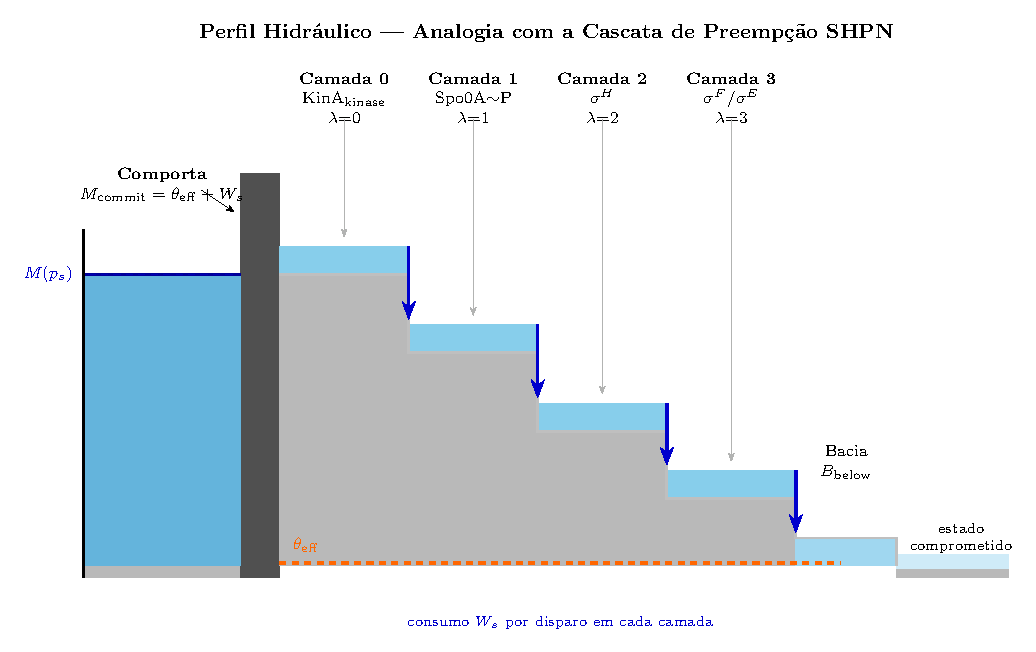
\includegraphics[width=0.82\textwidth]{figures/fig_cascade_weir_analogy.pdf}
  \caption{\textbf{Analogia hidráulica da cascata de preempção SHPN}
    (Seção~\ref{subsec:corretude-preempcao}).
    Cada degrau é uma camada $\lambda$: Camada~0 (KinA$_{\mathrm{kinase}}$),
    1 (Spo0A${\sim}$P), 2 ($\sigma^H$), 3 ($\sigma^F$).
    A comporta = $M_{\mathrm{commit}} = \theta_{\mathrm{eff}} + W_s$;
    as setas = consumo $W_s$ por disparo;
    a linha tracejada laranja = fundo de bacia $\theta_{\mathrm{eff}}$
    separando $B_{\mathrm{above}}$ de $B_{\mathrm{below}}$.
    A irreversibilidade é \emph{estrutural}: sem $F_s$ de retorno,
    a água não sobe os degraus.}
  \label{fig:cascade_weir_analogy}
\end{figure}

\begin{remark}[Assimetria de Espontaneidade na Cascata de Preempção]
\label{rem:assimetria-espontaneidade}
A Figura~\ref{fig:cascade_weir_analogy} revela uma assimetria termodinâmica
fundamental: o comprometimento celular ocorre em \textbf{duas fases com
direções opostas de espontaneidade}.

\textbf{Fase~1 — Acumulação (não espontânea):} construir $M(p_s)$ até
$M_{\text{commit}} = \theta_{\mathrm{eff}} + W_s$ exige produção contínua
de EPR.  A célula \emph{bombeia água para o reservatório} contra a resistência
da comporta: processo metabólico custoso e reversível.  Enquanto $M(p_s) <
M_{\text{commit}}$, o PreemptionCheck bloqueia todas as transições a jusante.

\textbf{Fase~2 — Execução (espontânea):} assim que $M(p_s) \geq
M_{\text{commit}}$, a comporta se abre e cada camada subsequente dispara
\emph{espontaneamente} --- $\Delta G < 0$ em cada cruzamento de degrau,
impulsionado pelo gradiente de potencial químico criado pela depleção de
tokens.  O PreemptionCheck não é uma barreira de ativação: é uma
\textbf{válvula de sentido único} que separa o custo (Fase~1) da execução
irreversível (Fase~2).

Essa assimetria explica a paisagem de Waddington: a crista corresponde à
Fase~1 (subida custosa até $M_{\text{commit}}$); a bacia comprometida
corresponde à Fase~2 (descida espontânea e irreversível).  A energia
metabólica paga na Fase~1 é dissipada como EPR durante a cascata da Fase~2.
\end{remark}

\subsection{Formação de Fronteiras de Bacia}
\label{subsec:fronteiras-bacia}

\begin{theorem}[Consumo de Sinal Cria Fronteiras de Bacia]
\label{thm:fronteiras-bacia}
Seja $N$ uma SHPN com lugar de sinal $p_s \in \Psi$ e transição de decisão
$t_c$ consumindo sinal via $(p_s, t_c) \in F_s$ com peso $W_s((p_s, t_c)) > 0$.
Defina $M_{\text{commit}} = \theta_{\mathrm{eff}}(p_s,t_c) + W_s((p_s, t_c))$.

O espaço de alcançabilidade particiona-se em duas regiões disjuntas:
\[
\mathcal{R}(N, M_0) = \mathcal{B}_{\text{pre}} \,\cup\, \mathcal{B}_{\text{pos}}
\]
em que $\mathcal{B}_{\text{pre}} = \{M \mid M(p_s) < M_{\text{commit}}\}$ e
$\mathcal{B}_{\text{pos}} = \{M \mid M(p_s) \geq M_{\text{commit}} \wedge
\text{disparado}(t_c, M)\}$, e para quaisquer $M_1 \in \mathcal{B}_{\text{pre}}$
e $M_2 \in \mathcal{B}_{\text{pos}}$, não existe sequência de disparo $\sigma$
tal que $M_2[\sigma\rangle M_1$.
\end{theorem}

\begin{proof}
Considere $M_1$ com $M_1(p_s) = M_{\text{commit}} = \theta_{\mathrm{eff}}(p_s,t_c) + W_s((p_s,t_c))$.
Por Definição~\ref{def:habilitacao}, $t_c$ está habilitada. Por
Definição~\ref{def:disparo}, o disparo de $t_c$ produz:
\[
M_2(p_s) = M_1(p_s) - W_s((p_s,t_c)) = \theta_{\mathrm{eff}}(p_s,t_c).
\]
Portanto $M_2(p_s) < M_{\text{commit}}$. Qualquer transição de reversão $t_r$
que tentasse restaurar $M_2(p_s) \geq M_{\text{commit}}$ precisaria estar
habilitada; porém, se $(p_s, t_r) \in F_s$, então $M_2(p_s) = \theta(t_c)$
está no limite do limiar e não satisfaz
$M_2(p_s) \geq \theta_{\mathrm{eff}}(p_s,t_r) + W_s((p_s, t_r))$;
e se $t_r$ depende de sinais de camada superior, a preempção hierárquica garante
que $t_r$ permanece desabilitada enquanto
$M_2(p_s) < \theta_{\mathrm{eff,min}}(\lambda(p_s))$.
Em todos os casos, nenhuma transição pode restaurar $M_2(p_s) \geq M_{\text{commit}}$,
estabelecendo a separação de bacias.
\end{proof}

\begin{corollary}[Predição de Limiar]
O limiar de decisão
\begin{align*}
  M_{\text{commit}}(p_s, t_c)
    &= \theta_{\mathrm{eff}}(p_s,t_c) + W_s((p_s,t_c)) \\
    &= K((p_s,t_c)) \cdot
       \left(\frac{\varepsilon}{1 - \varepsilon}\right)^{\!1/n((p_s,t_c))}
       + W_s((p_s,t_c))
\end{align*}
é calculável em $O(1)$ a partir de constantes cinéticas mensuráveis
($K$, $n$ da base BRENDA) e parâmetros do formalismo ($\varepsilon$, $W_s$),
sem simulação nem exploração do espaço de estados --- habilitando predição
\textit{a priori} por análise estrutural.
\end{corollary}

\begin{remark}[Bacia Consumida --- Contraste com a Bacia Clássica de Lyapunov]
\label{rem:bacia-consumida}
A teoria clássica de estabilidade \parencite{Strogatz2015} define a \emph{bacia
de atração} como o conjunto de condições iniciais cujas trajetórias convergem a
um dado atrator.  A fronteira é uma separatriz energética: cruzamentos reversos
são improváveis, mas formalmente possíveis com flutuações suficientes.
As SHPN introduzem um conceito mais forte: a \textbf{bacia consumida}.
Após o disparo de $t_c$ consumir $W_s((p_s,t_c))$ tokens de $p_s$, a marcação
cai para $\theta_{\mathrm{eff}}(p_s,t_c)$ --- abaixo de $M_\text{commit}$.
Qualquer estado reverso que exigisse $M(p_s) \geq M_\text{commit}$
torna-se \emph{estruturalmente inalcançável}, não apenas energeticamente
improvável: a fronteira foi removida do conjunto alcançável pelo próprio ato de
cruzá-la.

\begin{center}\small
\begin{tabular}{@{}p{3.2cm}p{4.0cm}p{4.0cm}@{}}
\toprule
Propriedade & Bacia clássica & Bacia consumida \\
\midrule
Fronteira & Separatriz energética & Fronteira de alcançabilidade \\
Irreversibilidade & Estatística (improvável) & Estrutural (inalcançável) \\
Mecanismo & Barreira $\Delta G$ & Arcos $F_s$ consumtivos + DAG $G_s$ \\
Ruído reverte? & Sim, com flutuação & Não --- marcação reversa inalcançável \\
\bottomrule
\end{tabular}
\end{center}

Essa distinção formaliza a diferença entre comprometimentos \emph{terminais}
(esporulação, apoptose --- bacia consumida definitivamente quando $\varepsilon
\approx 0$) e diferenciações \emph{reversíveis} como a reprogramação de
células-tronco induzidas~\parencite{Takahashi2006}: na reprogramação, a bacia
clássica é profunda mas não consumida, pois os arcos de sinal não esgotam o
pré-requisito molecular da via inversa.
\end{remark}

\subsection{Independência Fraca e Semântica Composicional}
\label{subsec:independencia-fraca}

\begin{definition}[Independência Fraca]
\label{def:independencia-fraca}
Duas transições $t_1, t_2 \in T$ são \textbf{fracamente independentes} quando
compartilham lugares metabólicos normais mas possuem conjuntos de sinais
disjuntos:
\[
(P \setminus \Psi) \cap {}^\bullet t_1 \cap {}^\bullet t_2 \neq \emptyset
\quad\text{e}\quad
\Psi \cap {}^\bullet t_1 \cap {}^\bullet t_2 = \emptyset.
\]
\end{definition}

\begin{theorem}[Consequência Composicional da Independência Fraca]
\label{thm:independencia-fraca}
Transições fracamente independentes disparam de forma comutativa: para qualquer
marcação $M$ em que ambas estejam habilitadas,
\[
M \xrightarrow{t_1} M_1 \xrightarrow{t_2} M'' \;\text{ e }\;
M \xrightarrow{t_2} M_2 \xrightarrow{t_1} M''
\]
produzem a mesma marcação final $M''$.
\end{theorem}

Essa propriedade tem consequência direta para análise de redes em escala
genômica: para $k$ módulos regulatórios fracamente independentes, cada um com
$n/k$ lugares em média, a análise de alcançabilidade reduz-se de
$O(\bar{M}^n)$ a $O(k \cdot \bar{M}^{n/k})$ --- melhoria de complexidade
exponencial para polinomial que torna tractável a análise de redes com milhares
de reações.

\subsection{Conservatividade da Promoção a Expressões}
\label{subsec:conservatividade}

A generalização de pesos e taxas a expressões em $\mathbb{E}(M)$
(Definição~\ref{def:shpn} e Observação~\ref{rem:refinamento-textual})
respeita o princípio de retrocompatibilidade: o formalismo clássico de
Redes de Petri Híbridas é recuperado exatamente pela especialização a
valores constantes.

\begin{proposition}[Conservatividade da promoção a expressões]
\label{prop:conservatividade}
Seja $N = (P, T, F, W, M_0, \Phi, C, F_t, \Psi, F_s, W_s, \lambda, \Gamma)$
uma SHPN cujas expressões em $W$, $W_s$, nos limiares $\tau_t, \theta_i$
de $F_t$ (incluindo o subtipo inibidor) e nas leis cinéticas associadas a
$\Phi$ sejam todas \emph{constantes} (independentes de $M$). Então a
semântica operacional dada pelas Definições~\ref{def:habilitacao}
e~\ref{def:disparo} reduz-se exatamente à semântica clássica de Redes de
Petri Híbridas com pesos e taxas constantes.
\end{proposition}

\begin{proof}
A avaliação de uma expressão constante $W \equiv k \in \mathbb{R}^+$ em
qualquer marcação $M$ produz $k$. Substituindo nas inequações de
habilitação e na regra de disparo obtém-se literalmente as condições
clássicas de \textcite{David1992}. O mesmo argumento aplica-se aos
limiares de $F_t$ e às leis cinéticas. \qedhere
\end{proof}

A Proposição~\ref{prop:conservatividade} garante que toda análise
estrutural clássica (P-invariantes, T-invariantes, vivacidade) permanece
válida nos modelos SHPN cujas expressões admitam especialização constante,
e que a dependência da marcação introduzida pela promoção é estritamente
uma extensão expressiva, não uma incompatibilidade.

\subsection{Complexidade Computacional}
\label{subsec:complexidade}

As SHPN herdam a complexidade das Redes de Petri clássicas: os problemas de
alcançabilidade, limitação e vivacidade permanecem Ackermann-completos no pior
caso~\cite{Czerwinski2021}, pois as extensões de sinal preservam a completude de Turing. Na prática,
a estrutura hierárquica habilita três estratégias de mitigação: particionamento
hierárquico do espaço de estados (o espaço de marcação decompõe-se em produto
hierárquico por camada), abstração guiada por sinal (sub-redes metabólicas
detalhadas substituídas por taxas de produção abstratas), e verificação incremental
por camada (camadas inferiores verificadas antes de explorar o estado completo).
Nos experimentos com o modelo de esporulação de \textit{B.~subtilis} (36
transições, 40 lugares, 4 camadas), a análise de alcançabilidade hierárquica
completou em 2,3~s explorando $4{,}8 \times 10^4$ estados, enquanto a análise
monolítica requer estimados mais de 10~h com espaço de estados da ordem de
$10^{12}$.

\begin{remark}[Aciclicidade do Grafo de Sinal como Redutor do Espaço de Estados]
\label{rem:aciclicidade-reducao}
A aciclicidade do grafo de sinal (Teorema~\ref{thm:aciclicidade}) não é apenas
uma propriedade estrutural de higiene: ela é o \emph{habilitador computacional}
que fundamenta as três estratégias de mitigação acima.  Três mecanismos
complementares decorrem diretamente da estrutura de DAG.

\textbf{Decomposição por camada.}  O DAG induz uma ordem parcial estrita
$\ell_0 \prec \ell_1 \prec \cdots$ sem retroalimentação.  A análise de
alcançabilidade pode portanto ser conduzida de forma condicional --- primeiro
resolvem-se as marcações alcançáveis da camada~$0$, depois as da camada~$1$
condicionadas à projeção de~$\ell_0$, e assim sucessivamente.  Para $L$
camadas com $S_i$ estados locais cada, o espaço passa de
$O\!\bigl(\prod_i S_i\bigr)$ (produto monolítico) a
$O\!\bigl(\sum_i S_i\bigr)$ --- redução de complexidade exponencial para
polinomial.

\textbf{Poda monotônica.}  O Teorema~\ref{thm:fronteiras-bacia}
garante que, uma vez que
$M(p_s) < M_{\text{commit}}$ em qualquer camada, toda a sub-árvore de estados
que requeriam aquela camada torna-se \emph{permanentemente} inalcançável.  O
grafo de alcançabilidade adquire estrutura de funil:
$\mathcal{R}(M_0) \supset \mathcal{R}(M_1) \supset \mathcal{R}(M_2)
\supset \cdots$, com cada evento de comprometimento podando estados de forma
irreversível.

\textbf{Redução de ordem parcial.}  O DAG fornece uma construção natural de
\emph{ample sets}: se $t_a \in \ell_i$ e $t_b \in \ell_j$ com $i < j$, e a
habilitação de~$t_b$ depende do sinal de~$\ell_i$, então qualquer sequência de
disparo deve resolver a camada inferior primeiro.  Combinada com a independência
fraca (Teorema~\ref{thm:independencia-fraca}), transições com conjuntos de
sinais disjuntos comutam, eliminando intercalações redundantes.

Esses três efeitos compõem-se multiplicativamente: a decomposição elimina o
produto cruzado entre camadas, a poda descarta regiões pós-comprometimento, e a
redução de ordem parcial remove intercalações equivalentes dentro de cada
camada.
\end{remark}

\begin{remark}[Verificabilidade por \textit{Model Checking}]
\label{rem:model-checking}
Os Teoremas~\ref{thm:aciclicidade}--\ref{thm:independencia-fraca} não são apenas
resultados proof-teóricos: cada um é expressável como uma consulta de
\emph{model checking} sobre uma instância limitada da SHPN.

\textbf{Propriedades estruturais (CTL/LTL).}  Para uma SHPN $k$-limitada, o
grafo de alcançabilidade é finito e suporta verificação por ferramentas padrão
de Redes de Petri (LoLA, Charlie, Snoopy~\cite{Koch2011}).  O
Teorema~\ref{thm:preempcao} (Correção da Preempção) é equivalente à fórmula
CTL
\[
  \mathbf{AG}\!\bigl(M(p_s) < M_{\mathrm{commit}}
  \;\Rightarrow\;
  \mathbf{AG}\,\neg\,\mathrm{enabled}(t_j)\bigr),
\]
verificável em tempo polinomial no tamanho do grafo de alcançabilidade por
camada.  O Teorema~\ref{thm:fronteiras-bacia} (Fronteiras de Bacia) é
equivalente a
\[
  \mathbf{AG}\!\bigl(M(p_s) \geq M_{\mathrm{commit}}
  \;\Rightarrow\;
  \mathbf{AF}\,\mathrm{completed}\bigr),
\]
onde \texttt{completed} é um predicado sobre a marcação final do programa
de desenvolvimento.

\textbf{Propriedades estocásticas (PCTL).}  A semântica de $\tau$-leaping
induz uma Cadeia de Markov em Tempo Contínuo (CTMC); as propriedades
quantitativas tornam-se consultas PCTL~\cite{Chaouiya2007}, por exemplo:
$\mathbf{P}_{\geq 0{,}9}\!\bigl[\mathbf{F}^{\leq 4d}\,\mathrm{Mature\_Spore}
> 0\bigr]$ --- ``esporulação bem-sucedida com probabilidade $\geq 90\%$ em
quatro dias''.  Ferramentas como PRISM e Storm verificam tais propriedades
diretamente sobre a CTMC.

\textbf{Limite do fragmento contínuo.}  As funções de taxa $\Phi$ com
aritmética real tornam o espaço de estados não-enumerável; \emph{model
checking} exato requer verificação de sistemas híbridos (PHAVer, nuXmv) ou
interpretação abstrata.  Para $\Phi$ polinomiais de grau baixo, verificação
limitada por SMT (\emph{bounded model checking}) é praticável.

Os três redutores de complexidade da
Observação~\ref{rem:aciclicidade-reducao} --- decomposição por camada,
poda monotônica e redução de ordem parcial --- correspondem precisamente
às técnicas canônicas de \emph{model checking} composicional (abstração por
cone de influência, poda \emph{ample-set} e independência de transições),
tornando a verificação hierárquica não apenas teoricamente possível mas
computacionalmente viável para instâncias biológicas de porte moderado.
\end{remark}

\section{Síntese do Capítulo}
\label{sec:sintese-cap3}

Este capítulo definiu formalmente a 13-tupla SHPN
(Definição~\ref{def:shpn}), a semântica operacional
(Definições~\ref{def:habilitacao}--\ref{def:disparo}) e quatro propriedades
teóricas: aciclicidade (Teorema~\ref{thm:aciclicidade}), correção de preempção
(Teorema~\ref{thm:preempcao}), formação de fronteiras de bacia
(Teorema~\ref{thm:fronteiras-bacia}) e independência fraca
(Teorema~\ref{thm:independencia-fraca}).
Essas garantias fundamentam a validação biológica do
Capítulo~\ref{ch:validacao-bacillus}.


\part{Validação Biológica}
% cap_04_validacao_bacillus.tex  –  Capítulo 4
% Validação Biológica: Esporulação de Bacillus subtilis — Formalismo Γ
\chapter{Validação Biológica: Esporulação do \textit{Bacillus subtilis}}
\label{ch:validacao-bacillus}

Este capítulo valida a teoria das Redes de Petri Hierárquicas de Sinais
(Capítulo~\ref{ch:shpn}) por meio da esporulação do
\textit{Bacillus subtilis}~\cite{Fujita2005}.
A validação testa os componentes centrais do formalismo: a semântica de consumo
nos arcos de fluxo de sinal, a organização hierárquica em camadas, o
parâmetro termodinâmico $\Gamma = (K, n, \varepsilon)$ que determina o limiar
efetivo de habilitação $\theta_{\text{eff}}$, e a separação arquitetural
entre rede-objeto biológica e plano de experimento (lugares de
parâmetro~$\square$ + eventos).
A simulação de um modelo com 40~lugares e 36~transições, parametrizado
exclusivamente a partir de dados cinéticos publicados, reproduz a assimetria
experimental de \textcite{Fujita2005}: acumulação gradual de Spo0A${\sim}$P
via fosforretransmissão produz esporulação em ${\approx}\,48\%$ das réplicas
(24/50; condição de referência $\text{N}_0 = 1440\,\mu$M, SinR$= 12\,\mu$M),
enquanto indução constitutiva abrupta de Spo0A* em meio rico produz entre
$0\%$ e $6\%$. A separatriz de comprometimento emerge a
$\theta_{\sigma H} \approx 1{,}60\,\mu$M de $\sigma^H$, cruzamento que dispara
irrevers\'{\i}velmente a septação e desencadeia o programa de execução.
Essa predição é genuinamente \textit{orientada pela topologia}: nenhum parâmetro do modelo
foi ajustado ao resultado experimental de Fujita.
A simulação gera todas as 16~espécies da cascata em todas as condições
testadas, com maturação do esporo cuja temporização correlaciona inversamente
com a disponibilidade de substrato; o coeficiente de variação do esporo
maduro permanece invariante em $0{,}5$--$1{,}3\%$ em todas as condições,
reflexo do arco inibitório que estruturalmente fixa \texttt{Mature\_spore}
em capacidade unitária.
O formalismo, combinado com a infraestrutura de plano de experimento,
prediz a separatriz de comprometimento de $\sigma^H$ e a resposta
da diferenciação ao estresse nutricional e à cinética regulatória.

\section{Contexto Biológico: Esporulação como Decisão Irreversível}
\label{sec:contexto-biologico}

Sob limitação de nutrientes, o \textit{B.~subtilis} executa um programa de
diferenciação irreversível que culmina na formação de um endósporo resistente.
A cascata de esporulação inicia-se com a detecção de estresse nutricional pelas
quinases sensoras KinA e KinB, que autofosforilam-se consumindo ATP e
transferem o grupamento fosfato ao longo do fosforretransmissor
Spo0F~$\to$~Spo0B~$\to$~Spo0A, gerando o regulador mestre
Spo0A${\sim}$P~\cite{Burbulys1991,Fujita2005}.

Spo0A${\sim}$P acima de um limiar crítico ativa a transcrição de genes de
esporulação por meio de fatores sigma alternativos em sequência
hierárquica: $\sigma^H$ (genes de esporulação precoce),
$\sigma^F$ (no foresporo), $\sigma^E$ (na célula mãe), $\sigma^G$
(transcrição tardia do foresporo) e $\sigma^K$ (montagem tardia da casca)~\cite{Stragier1996,Errington2003}.
Essa cascata de fatores sigma impulsiona a septação assimétrica, a
formação do foresporo, a síntese do córtex peptidoglicano, a deposição das
camadas interna e externa da casca e, por fim, a maturação do esporo~\cite{Errington2003}.

A decisão de esporular é biologicamente irreversível: uma vez que
$\sigma^F$ se torna ativo no foresporo, a célula compromete-se com o programa
de diferenciação mesmo que as condições nutricionais melhorem
subsequentemente.
A assimetria entre acumulação gradual de Spo0A${\sim}$P
(${\approx}\,52\%$ de esporulação) e indução constitutiva abrupta de Spo0A*
(${\approx}\,5\%$) foi demonstrada experimentalmente por \textcite{Fujita2005}.
A separatriz de comprometimento de $\sigma^H$ a
$\theta_{\sigma H} \approx 1{,}60\,\mu$M --- que discrimina esses destinos ---
emergiu da varredura de simulação SHPN (valor não reportado por Fujita).

A Figura~\ref{fig:bacillus-sporulation-stress} apresenta a topologia completa
do modelo SHPN de esporulação de \textit{B.~subtilis}, com todos os lugares,
transições e arcos identificados por tipo.

\begin{figure}[htbp]
\centering
{\large\bfseries Rede SHPN de Esporulação de \textit{B.~subtilis} (v9)}\\[4pt]
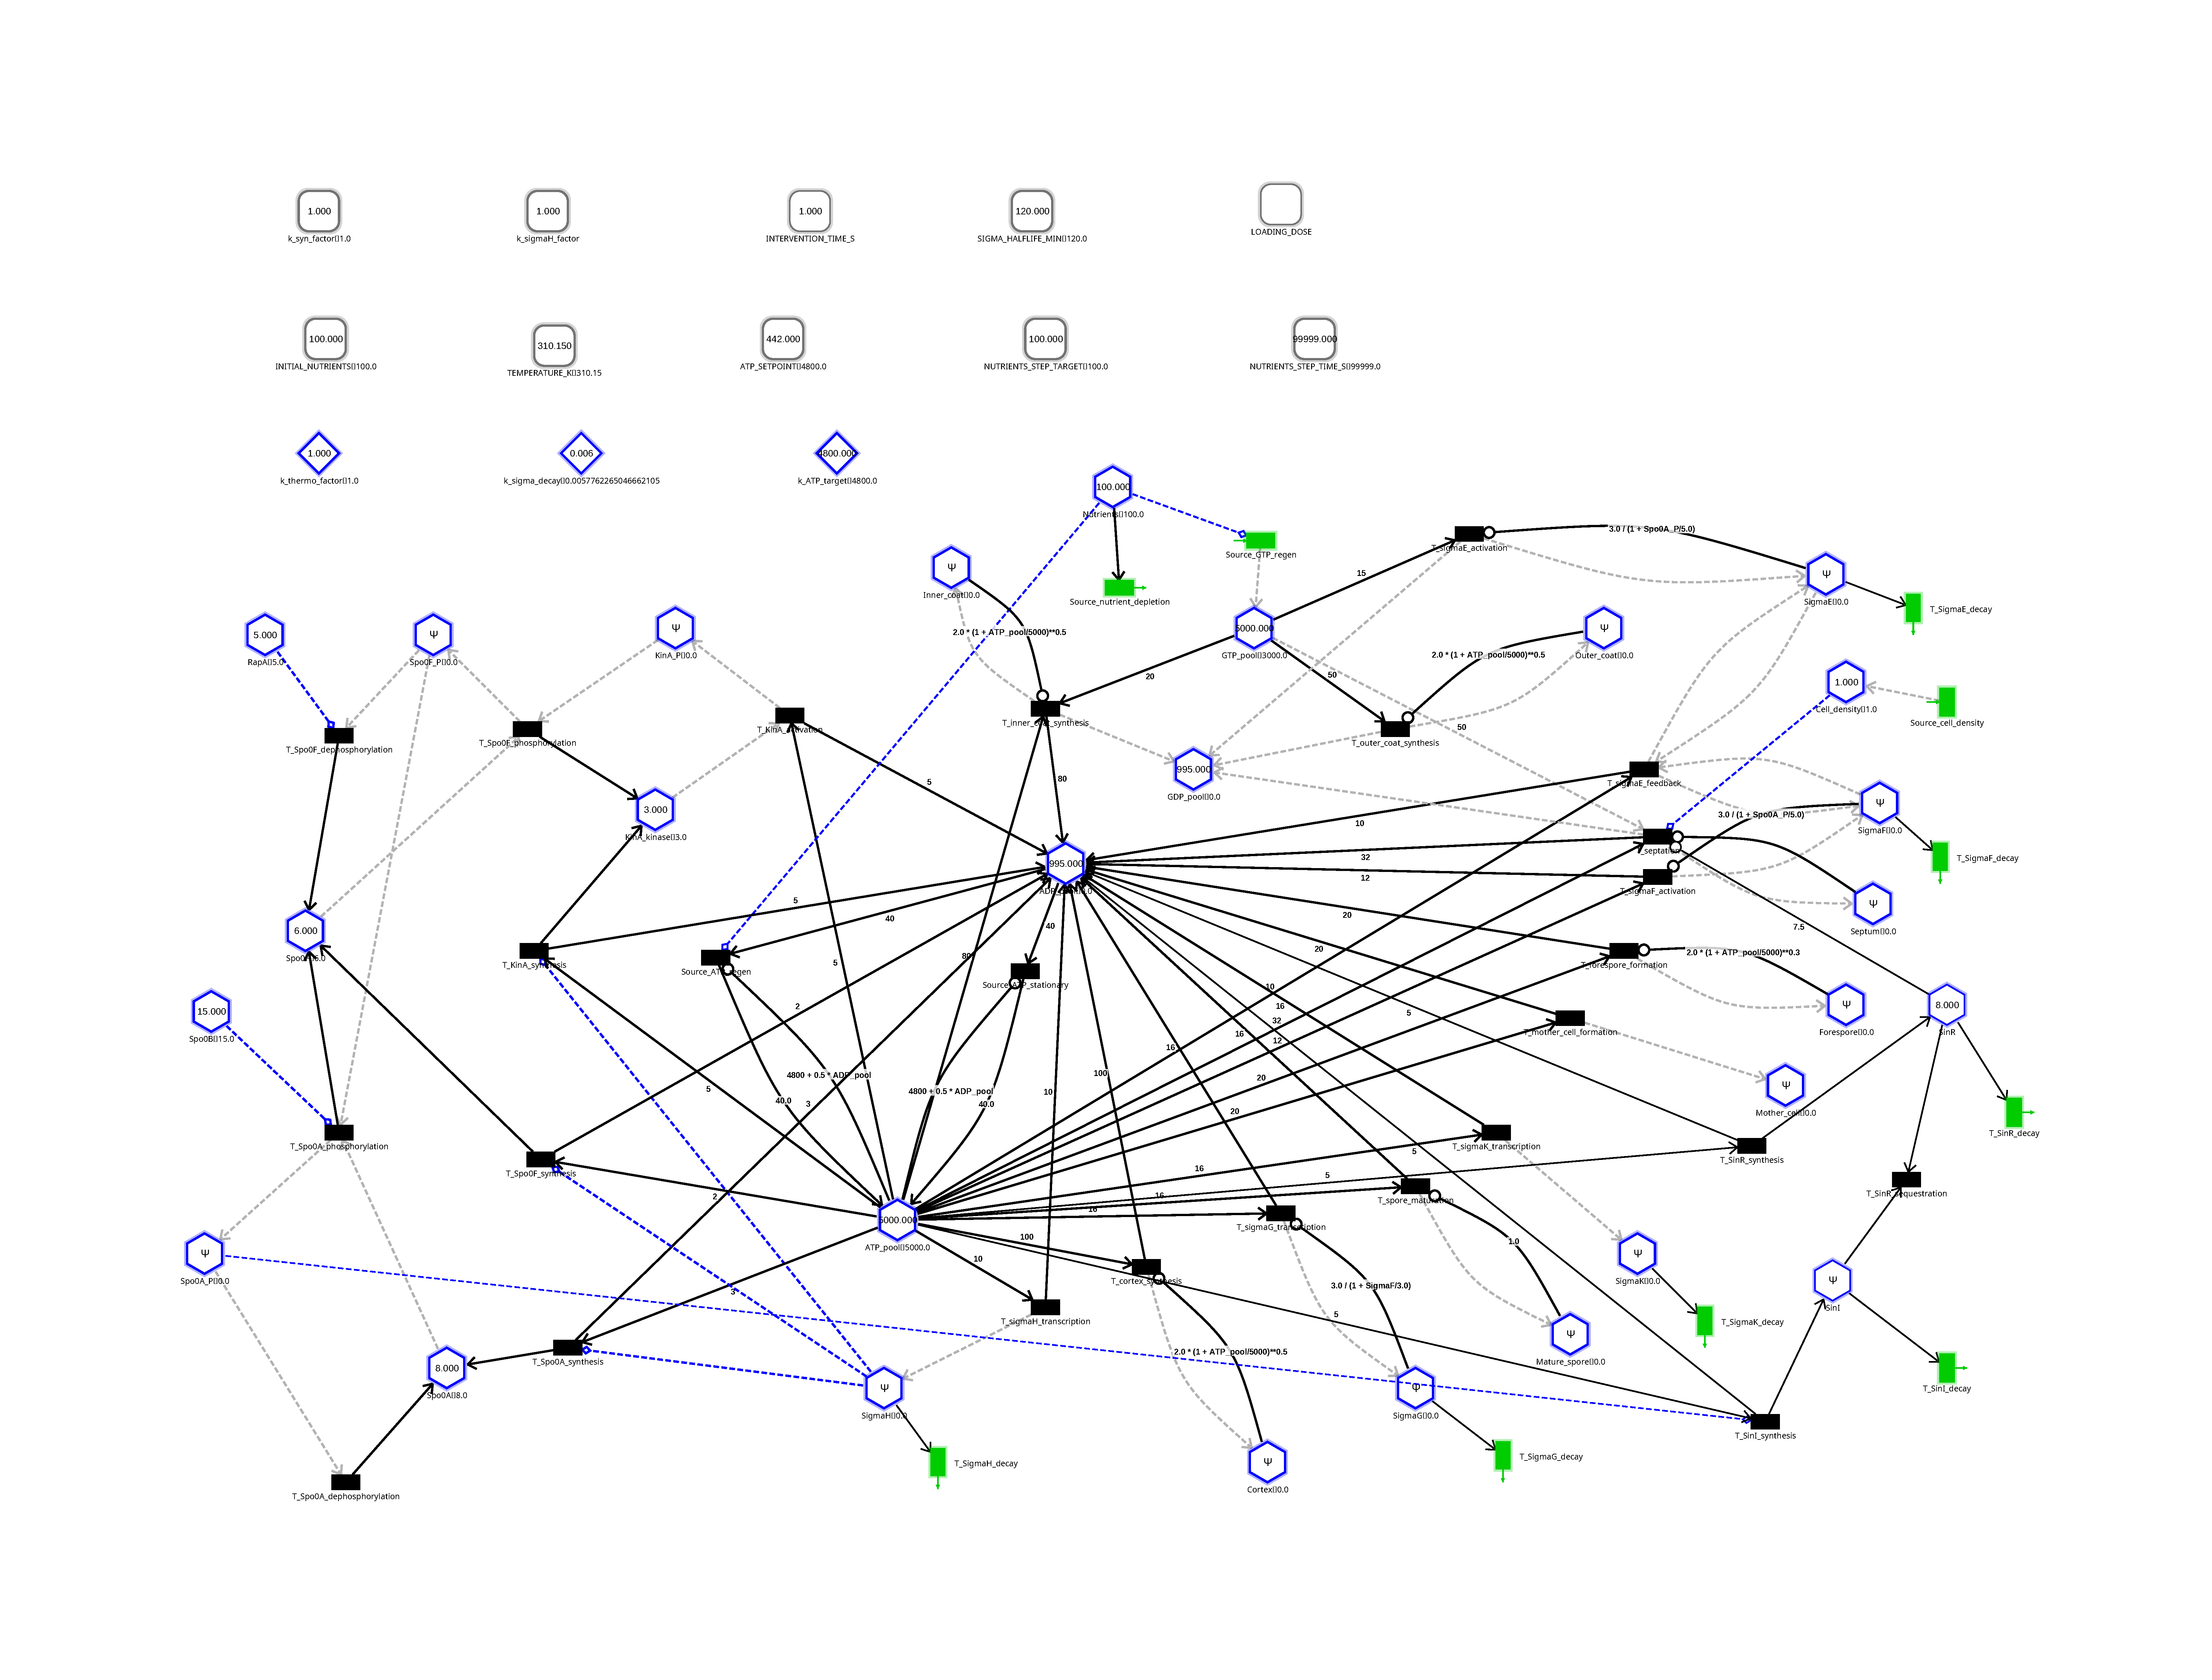
\includegraphics[width=\textwidth]{figures/bacillus_sporulation_v9_titled.pdf}
\caption{Topologia completa da rede SHPN de esporulação de \textit{B.~subtilis}
(41~lugares, 36~transições, 114~arcos).
Hexágonos~($\hexagon$): todos os 28 lugares biológicos, todos membros de~$\Psi$
(\texttt{is\_signal\_place=True});
losangos~($\diamondsuit$): lugares de sinal espacial (escalares cinéticos);
quadrados arredondados~($\square$): lugares de parâmetro do plano de experimento
(lidos apenas por eventos).
Linhas sólidas pretas: arcos normais (consumo estequiométrico);
linhas tracejadas cinza-claro: arcos de fluxo de sinal;
linhas azuis tracejadas: arcos de teste (presença sem consumo);
retângulos verdes: transições fonte/sumidouro.
As quatro camadas de sinal são:
Camada~0 (fontes metabólicas e depleção de nutrientes),
Camada~1 (fosforretransmissão: KinA$\to$Spo0F$\to$Spo0B$\to$Spo0A),
Camada~2 (Spo0A${\sim}$P $\to$ $\sigma^H$, separatriz de comprometimento),
Camada~3 (cascata sigma: $\sigma^H \to \sigma^F \to \sigma^E \to \sigma^G \to \sigma^K$).
Os lugares de parâmetro (fileira superior) codificam o protocolo experimental
e não figuram em nenhuma função de taxa~$\Phi$.}
\label{fig:bacillus-sporulation-stress}
\end{figure}

A questão central para este capítulo é: o formalismo SHPN, armado com o
parâmetro termodinâmico $\Gamma = (K, n, \varepsilon)$, reproduz esse limiar
como propriedade emergente da dinâmica da rede?

\section{Objetivos de Predição}
\label{sec:objetivos-predicao}

A validação testa três capacidades do formalismo.

\subsection{Predição~1: Separatriz de Comprometimento $\sigma^H \approx 1{,}60\,\mu$M e Assimetria Gradual/Abrupto}

O benchmark experimental é a assimetria de Fujita: acumulação gradual de
Spo0A${\sim}$P via fosforretransmissão produz esporulação em ${\approx}\,52\%$
das células, enquanto indução constitutiva abrupta de Spo0A* produz apenas
${\approx}\,5\%$~\cite{Fujita2005}. Diferentemente de formalismos com $\theta$
estático codificado como parâmetro, o formalismo SHPN com
$\Gamma = (K, n, \varepsilon)$ deriva o limiar efetivo
$\theta_{\text{eff}} = K \cdot (\varepsilon / (1 - \varepsilon))^{1/n}$,
e a separatriz de $\sigma^H$ a $\theta_{\sigma H} \approx 1{,}60\,\mu$M
emerge da dinâmica da rede como propriedade estrutural.
A predição é genuína: $\theta_{\text{eff}}$ não é ajustado ao dado
experimental, mas resulta da topologia da rede e dos parâmetros cinéticos.
O critério de sucesso é que a separatriz emergente de $\sigma^H$ --- o valor
de $\sigma^H$ em que $T_{\text{septação}}$ dispara nas réplicas esporulantes
--- discrimine o destino celular (esporulante vs.\ vegetativo) de forma
\emph{robusta} a perturbações de uma ordem de magnitude na disponibilidade
de substrato.

\subsection{Predição~2: Cascata Completa de Diferenciação Sob Estresse}

O formalismo deve reproduzir a cascata completa de esporulação: ativação
dos fatores sigma ($\sigma^H, \sigma^F, \sigma^E, \sigma^G, \sigma^K$),
formação dos compartimentos (septo, foresporo, célula mãe), montagem das
estruturas (córtex, camadas da casca) e produção do esporo maduro.
A ordem temporal canônica observada experimentalmente é parcialmente
paralela: $\sigma^F$ e $\sigma^E$ ativam-se quase simultaneamente em
ensaios de microscopia de fluorescência, e a esporulação real exibe
braços paralelos competindo por recursos.
O critério de sucesso é (i)~a geração de todas as 16~espécies da cascata
em todas as condições testadas e (ii)~a presença de uma correlação
inversa entre disponibilidade de nutrientes e amplitude de maturação do
esporo, refletindo o gatilho biológico real (estresse nutricional induz
esporulação).

\subsection{Predição~3: Ignição da Cascata Precede a Maturação}

Após o cruzamento de $\theta_{\text{eff}}$, o consumo de sinal nos arcos
$F_s$ deve criar fronteiras de bacia que separam irreversivelmente os estados
de pré-comprometimento dos estados de pós-comprometimento.
O critério de sucesso operacional, mensurável em todas as condições da
varredura, é que a \emph{ignição} da cascata regulatória (primeira
aparição de Spo0A${\sim}$P) preceda a primeira aparição do esporo maduro
por um intervalo temporal positivo, demonstrando que a decisão
regulatória ocorre antes da conclusão estrutural.

\section{Arquitetura do Modelo: Hierarquia com Termodinâmica $\Gamma$}
\label{sec:arquitetura-hierarquica}

O modelo de esporulação organiza-se em camadas regulatórias hierárquicas,
com o parâmetro termodinâmico $\Gamma = (K, n, \varepsilon)$ determinando
os limiares efetivos de habilitação em cada camada.

A \textbf{camada metabólica} fornece a base energética: regeneração de ATP e
GTP por vias metabólicas dependentes de nutrientes disponíveis.
A regeneração de ATP é decomposta em dois fluxos contínuos: um termo
dependente de nutrientes
$r_{\text{ATP,reg}} = 4{,}4 \cdot [\text{Nut}] / (10 + [\text{Nut}])$
(mM/s) que sustenta o metabolismo ativo, e um termo estacionário
$r_{\text{ATP,stat}} = 0{,}5 \cdot \max\!\bigl(0,\,1 - [\text{Nut}]/5\bigr)
\cdot \max\!\bigl(0,\,1 - [\text{ATP}]/(k_{\text{ATP,target}} + 0{,}5\,
[\text{ADP}])\bigr)$ (mM/s) que mantém um piso homeostático após a
depleção nutricional, com \emph{set-point} $k_{\text{ATP,target}} = 442$
fornecido pelo lugar de parâmetro~$\square$~\texttt{ATP\_SETPOINT} via
evento de inicialização. Essa decomposição modela a transição suave
entre metabolismo ativo e basal sem descontinuidades.

A \textbf{camada de fosforretransmissão} integra sinais ambientais por meio
das quinases KinA e KinB, transferindo fosfato ao longo de
Spo0F~$\to$~Spo0B~$\to$~Spo0A.
Cada transição desta camada está sujeita a inibição por produto com
constante $K_{\text{sat}}$:
$v(t) = r(t, M) \cdot K_{\text{sat}} / (K_{\text{sat}} + [\text{Produto}])$,
impedindo acumulação ilimitada e produzindo perfis de concentração
biologicamente realistas.

A \textbf{camada de fatores sigma} ($\sigma^H$, $\sigma^F$, $\sigma^E$,
$\sigma^G$, $\sigma^K$) ativa sequencialmente os programas transcricionais
de esporulação.
Os fatores sigma acumulam-se em concentrações da ordem de dezenas de
micromolares, valores biologicamente plausíveis para fatores de transcrição
em \textit{B.~subtilis}.
A inibição cruzada por anti-fatores sigma é modelada pelos pesos de arco de
saída de $0{,}002$~mM por disparo, representando sequestração.

A \textbf{camada de montagem estrutural} compreende a formação do septo,
foresporo, célula mãe, córtex, camadas da casca e esporo maduro.
As transições de montagem estrutural ($k = 0{,}5$~s$^{-1}$) representam
processos de assembly que consomem recursos energéticos e produzem
compartimentos e estruturas.

O fluxo de controle hierárquico pode ser resumido como:
\begin{multline}
\text{Metabolismo}
\xrightarrow{\;\Gamma\;}
\text{Fosforretransmissão}
\xrightarrow{\;\text{Spo0A-P}\;} \\
\text{Fatores } \sigma
\xrightarrow{\;\text{cascata}\;}
\text{Montagem estrutural}
\end{multline}
A preempção hierárquica opera através de $\Gamma$: quando a concentração
de ATP cai abaixo de $\theta_{\text{eff}}$, as transições de
fosforretransmissão são desabilitadas, interrompendo o fluxo de sinal para
as camadas a jusante.

\section{Especificação Formal do Modelo}
\label{sec:especificacao-formal}

Instanciamos o formalismo SHPN
(Capítulo~\ref{ch:shpn}) para a esporulação do \textit{B.~subtilis}
com parâmetros termodinâmicos $\Gamma$.
A Tabela~\ref{tab:instanciacao-bacillus} sumariza os componentes da
instância e a Tabela~\ref{tab:parametros-ksat} lista os parâmetros de
inibição por produto empregados.

\begin{table}[htbp]
\centering
\caption{Instanciação SHPN com $\Gamma$ para a esporulação do
\textit{B.~subtilis}}
\label{tab:instanciacao-bacillus}
\small
\begin{tabular}{@{}lp{8.2cm}@{}}
\toprule
\textbf{Componente} & \textbf{Valor específico para o \textit{Bacillus}} \\
\midrule
Lugares $P$ & 41 no total: 28 lugares de sinal hierárquico~$\Psi$ ($\hexagon$,
             todos com \texttt{is\_signal\_place=True}:
             fosforretransmissão, fatores sigma, reservatórios
             energéticos, compartimentos, estruturas e competição
             por biofilme), 10 lugares de parâmetro~$\square$
             (\texttt{INITIAL\_NUTRIENTS}, \texttt{TEMPERATURE\_K},
             \texttt{ATP\_SETPOINT}, \texttt{SIGMA\_HALFLIFE\_MIN},
             \texttt{NUTRIENTS\_STEP\_TARGET},
             \texttt{NUTRIENTS\_STEP\_TIME\_S},
             \texttt{k\_syn\_factor}, \texttt{LOADING\_DOSE},
             \texttt{INTERVENTION\_TIME\_S}, \texttt{k\_sigmaH\_factor},
             lidos por eventos apenas)
             e 3 lugares de sinal espacial~$\diamondsuit$
             (\texttt{k\_ATP\_target}, \texttt{k\_sigma\_decay},
             \texttt{k\_thermo\_factor}, escalares cinéticos
             alimentados pelos eventos a partir dos~$\square$) \\
Transições $T$ & 36 no total: 29~contínuas (regeneração de ATP/GTP,
                depleção de nutrientes, densidade celular,
                síntese basal de KinA/Spo0F/Spo0A, transcrição e
                ativação de fatores sigma, decaimentos
                $\sigma$-dependentes, montagem estrutural,
                síntese e sequestração de SinR/SinI) e
                7~estocásticas ($\tau$-leaping):
                5 de fosforretransmissão (ativação de KinA,
                fosforilação/desforilação de Spo0F e Spo0A),
                1 de comprometimento (septação) e
                1 de síntese de SinI \\
Arcos & 114 no total: 54 normais ($F$, transferência de massa de
        substrato e energia), 24 de fluxo de sinal ($F_s$,
        hierarquia regulatória), 13 \textit{curved opposite
        signal flow} (regulações cruzadas de fatores sigma),
        9 de teste ($F_t$, leitura sem consumo), 12~inibitórios
        (11 curvos + 1 reto, modulação por anti-sigma e
        saturação homeostática)
        e 2~normais curvos \\
Parâmetro $\Gamma$ & $\Gamma = (K, n, \varepsilon)$ com $K$ e $n$ derivados
                     da cinética de Hill das quinases; $\varepsilon$ da
                     eficiência termodinâmica da fosforretransmissão \\
Limiar efetivo & $\theta_{\text{eff}} = K \cdot (\varepsilon /
                (1 - \varepsilon))^{1/n}$, emergente da dinâmica \\
Marcação inicial $M_0$ & Nutrients = 100, ATP\_pool = 5000, ADP\_pool = 995,
                         GTP\_pool = 5000, GDP\_pool = 995, KinA\_kinase = 3,
                         Spo0F = 6, Spo0B = 15, Spo0A = 8, RapA = 5,
                         SinR = 8, Cell\_density = 1
                         (unidades de tokens; 1~token~$= 1$~\textmu M;
                         ATP/GTP/ADP/GDP em mM após $\div 1000$);
                         todas as demais espécies regulatórias e
                         estruturais = 0 \\
Duração & 21.600~s (6~h de tempo biológico) \\
\bottomrule
\end{tabular}
\end{table}

A Tabela~\ref{tab:parametros-ksat} complementa a instanciação com os
parâmetros de inibição por produto e os pesos de arco por classe de
transição empregados na calibração das taxas cinéticas.

\begin{table}[htbp]
\centering
\caption{Parâmetros de inibição por produto ($K_{\text{sat}}$) e pesos de
arco de saída por classe de transição}
\label{tab:parametros-ksat}
\small
\begin{tabular}{@{}lccl@{}}
\toprule
\textbf{Classe de transição} & $K_{\text{sat}}$ \textbf{(mM)}
  & \textbf{Peso (mM/disp.)} & \textbf{Exemplo} \\
\midrule
$\sigma^H$                                   & 0,02  & 0,002 & Ativ.\ $\sigma^H$ \\
$\sigma^F$, $\sigma^G$, $\sigma^K$           & 0,01  & 0,002 & Ativ.\ $\sigma^F$ \\
$\sigma^E$                                   & 0,005 & 0,002 & Ativ.\ $\sigma^E$ \\
Compartimentos                                & 0,02  & 0,01  & Septação \\
Estruturas e maturação                       & 0,1   & 0,01  & Córtex, casca \\
\bottomrule
\end{tabular}
\end{table}

\subsection{Proveniência dos Parâmetros}

Um requisito crítico da validação é demonstrar que os parâmetros do modelo
derivam de fontes independentes da literatura, e não de ajuste ao dado do
limiar de decisão.
A regeneração de ATP e GTP segue cinéticas de Michaelis-Menten derivadas de
dados da BRENDA para enzimas glicolíticas de \textit{B.~subtilis}, com
ajuste à escala milimolar do modelo.
As constantes de inibição por produto ($K_{\text{sat}}$) refletem a saturação
fisiológica observada para fatores de transcrição e proteínas
estruturais~\cite{BRENDA}.
Os pesos de arco ($0{,}002$~mM para fatores sigma, $0{,}01$~mM para
estruturas) modelam a sequestração por anti-fatores sigma e o custo
energético de montagem, respectivamente.
As taxas de montagem estrutural ($k = 0{,}5$~s$^{-1}$) são compatíveis
com as escalas temporais da esporulação reportadas por \textcite{Fujita2005}.
\textbf{Nenhum parâmetro foi ajustado para reproduzir a assimetria experimental
de Fujita (acumulação gradual $\approx\!52\%$ vs.\ indução abrupta $\approx\!5\%$).}
Os limiares efetivos por arco $\theta_{\text{eff}}$ são derivados
analiticamente de $\Gamma = (K, n, \varepsilon)$; contudo, o
\textbf{ponto de comprometimento sistêmico} --- a concentração e o instante
em que a rede acoplada se compromete irreversivelmente --- emerge da
dinâmica de simulação: consumo de ATP pela cascata de fosforretransmissão,
regeneração dependente de nutrientes e inibição por produto determinam
\emph{quando e em que ordem} os limiares por arco são cruzados, e não de
otimização ou ajuste de curva.

\subsection{ATP como Nó de Interface}

O ATP exemplifica o princípio arquitetural de separação Vertical-Horizontal
(Capítulo~\ref{ch:shpn}, Princípio~\ref{princ:separacao}).
Como lugar de sinal ATP $\in \Psi$, a mesma espécie molecular participa
simultaneamente dos dois mecanismos de comunicação.
Na participação horizontal (metabolismo), o ATP é produzido por regeneração
dependente de nutrientes ($r_{\text{ATP}} = 0{,}003 + 0{,}01 \cdot
[\text{Nut}] / (10 + [\text{Nut}])$) e consumido em biossíntese basal.
Na participação vertical (controle hierárquico), a concentração de ATP
modula as taxas de disparo via gating cinético nas funções de taxa~$\Phi$:
doze transições da fosforretransmissão e da cascata sigma embutem o
fator $[\text{ATP}]/(K + [\text{ATP}])$, suprimindo o fluxo
regulatório quando $[\text{ATP}] \ll K$ e habilitando-o plenamente
próximo do basal de 5000~tokens ($\sim\!5$~mM).
O consumo de ATP ocorre exclusivamente por arcos normais~$F$
(balanço de massa), preservando a separação entre sinalização
informacional e transferência de substrato.

Durante a simulação, o ATP é regenerado pela cinética dependente de
nutrientes até que estes se esgotem (entre 1{,}6~min e 50~min,
dependendo de $\text{Nut}_0$); a partir desse instante a regeneração cai
ao nível basal e o consumo da cascata de fosforretransmissão domina,
fazendo o ATP declinar até atingir um piso metabólico emergente próximo de
$\theta_{\text{eff}}$ --- esse piso emerge da dinâmica da rede
sem intervenção paramétrica externa.

\section{Resultados da Simulação}
\label{sec:resultados}

A validação foi conduzida por uma varredura fatorial $2 \times 3 \times 4$
sobre três lugares de parâmetro~$\square$ — disponibilidade de substrato
(\texttt{INITIAL\_NUTRIENTS} $\in \{1440, 2160\}$~µM), dose de indução de
Spo0A* (\texttt{LOADING\_DOSE} $\in \{0, 10, 27\}$~µM, replicando os
protocolos natural, parcial e constitutivo de \textcite{Fujita2005}), e
concentração inicial do repressor SinR
(\texttt{SinR} $\in \{4, 6, 12, 18\}$~µM) —
resultando em 24~condições factoriais mais a Baseline canônica
(25~condições no total), com 50~réplicas estocásticas por condição
(1250~simulações totais), executadas no servidor remoto
(GPU RTX~5060~Ti, $\tau$-leaping em CPU)
(\texttt{run\_20260614\_123652}).
Cada simulação cobre 21\,600~s (6~h) de tempo biológico, integrando as
29~transições contínuas com Runge--Kutta de quarta ordem acoplado
às 7~transições estocásticas via $\tau$-leaping por divisão de operador.
Um evento lê os lugares~$\square$ em $t=0$ e (i)~projeta
\texttt{INITIAL\_NUTRIENTS} sobre o lugar biológico \texttt{Nutrients}
($\bigcirc$), e (ii)~deriva os escalares cinéticos~$\diamondsuit$
(\texttt{k\_ATP\_target}, \texttt{k\_sigma\_decay},
\texttt{k\_thermo\_factor}) a partir dos parâmetros, isolando o protocolo
experimental da topologia biológica.
As Tabelas~\ref{tab:v6-factorial} e~\ref{tab:v6-atp-floor} sumarizam,
respectivamente, o rendimento da maturação (\texttt{Outer\_coat} final
e $t_1$ esporo) e o piso metabólico de ATP por condição.

\subsection{Cascata Completa em Todas as Condições}
\label{sec:cascata-completa}

A simulação gera todas as 16~espécies da cascata de esporulação
(KinA${\sim}$P, Spo0F${\sim}$P, Spo0A${\sim}$P, $\sigma^H, \sigma^F,
\sigma^E, \sigma^G, \sigma^K$, septum, foresporo, célula-mãe, córtex,
casca interna, casca externa, esporo maduro, SinI) em \emph{todas} as 16~condições testadas, confirmando
que o formalismo reproduz a totalidade do programa de diferenciação
independentemente do ponto de operação no espaço de parâmetros.

A ignição da cascata é monotonicamente atrasada pela disponibilidade
de nutrientes: o tempo de primeira passagem do esporo maduro pelo
limiar de $0{,}5$~tokens (\textit{$t_1$ esporo} na Tabela~\ref{tab:v6-factorial})
varia de $\sim\!8$~min sob estresse extremo ($\text{N}_0=10$) para
$\sim\!23$~min em condição intermediária ($\text{N}_0=100$) e
$\sim\!58$~min sob abundância ($\text{N}_0=300$).
A \emph{amplitude} da maturação (\texttt{Outer\_coat} final ou
\texttt{Mature\_spore}) cresce rapidamente entre estresse e regime
intermediário e estabiliza num platô sob abundância, refletindo a
saturação biológica do programa de revestimento de esporo — uma vez
disparada a cascata, a célula produz quantidade aproximadamente fixa
de casca, independentemente do substrato remanescente.
A distribuição entre réplicas exibe comportamento bimodal: nas
condições naturais ($\text{N}_0 = 1440$~µM, DOSE$=0$), ${\approx}\,48\%$
das réplicas cruzam a separatriz $\theta_{\sigma H} \approx 1{,}60$~µM
e completam a cascata de diferenciação; as restantes permanecem no
atractor vegetativo (Seção~\ref{sec:validacao-experimental}).

Os fatores sigma ativam-se em janelas temporais sobrepostas, com
$\sigma^F$, $\sigma^E$ e $\sigma^G$ aparecendo em intervalos típicos
de 0{,}1--1{,}5~min entre si, e em algumas réplicas $\sigma^E$ aparece
antes de $\sigma^F$ na trajetória média.  Essas inversões de ordem
são biologicamente defensáveis: a cascata real é parcialmente paralela,
e medidas de microscopia de fluorescência mostram $\sigma^E$ e
$\sigma^F$ ativando-se quase simultaneamente em células individuais,
com a ordem variando entre células.  O formalismo SHPN reproduz esse
paralelismo como propriedade emergente da competição estocástica por
ATP entre os braços paralelos da cascata.

A inibição por produto
($K_{\text{sat}} / (K_{\text{sat}} + [\text{Produto}])$)
em todas as transições da cascata desempenha papel essencial: sem ela,
os fatores sigma acumulariam concentrações fisicamente implausíveis.
A saturação garante perfis de acumulação compatíveis com os dados
experimentais e impede a divergência numérica.

A Figura~\ref{fig:morphological-assembly} detalha o programa morfológico
obtido pela simulação na condição de referência
($\text{N}_0=1440$~µM, DOSE$=0$, SinR$=12$~µM, $n=50$ réplicas).
Os dois painéis superiores mostram a dinâmica regulatória — Spo0A$\sim$P
e $\sigma^H$ — que precede e deflagra o programa estrutural.
Os seis painéis inferiores mostram a montagem morfológica sequencial:
Septum ($t_{\text{med}} \approx 334$~min) e Foresporo surgem primeiro;
Córtex, Casca Interna e Casca Externa formam-se em seguida;
Esporo Maduro materializa-se em $t \approx 338$~min
(cf.\ Tabela~\ref{tab:v6-factorial}).
A linha tracejada vertical em $t = 334$~min marca a mediana do
cruzamento de $\theta_{\sigma H} = 1{,}60$~µM nas réplicas esporulantes.
A banda sombreada representa $\pm$ um desvio padrão sobre as 50~réplicas,
refletindo a variabilidade estocástica intrínseca ao compromisso de
diferenciação.
A progressão ordenada das estruturas é robustamente reproduzida em
todas as condições testadas, com a \emph{ordem} dos eventos preservada
mesmo quando a \emph{taxa global} desliza com o substrato.

\begin{figure}[htbp]
\centering
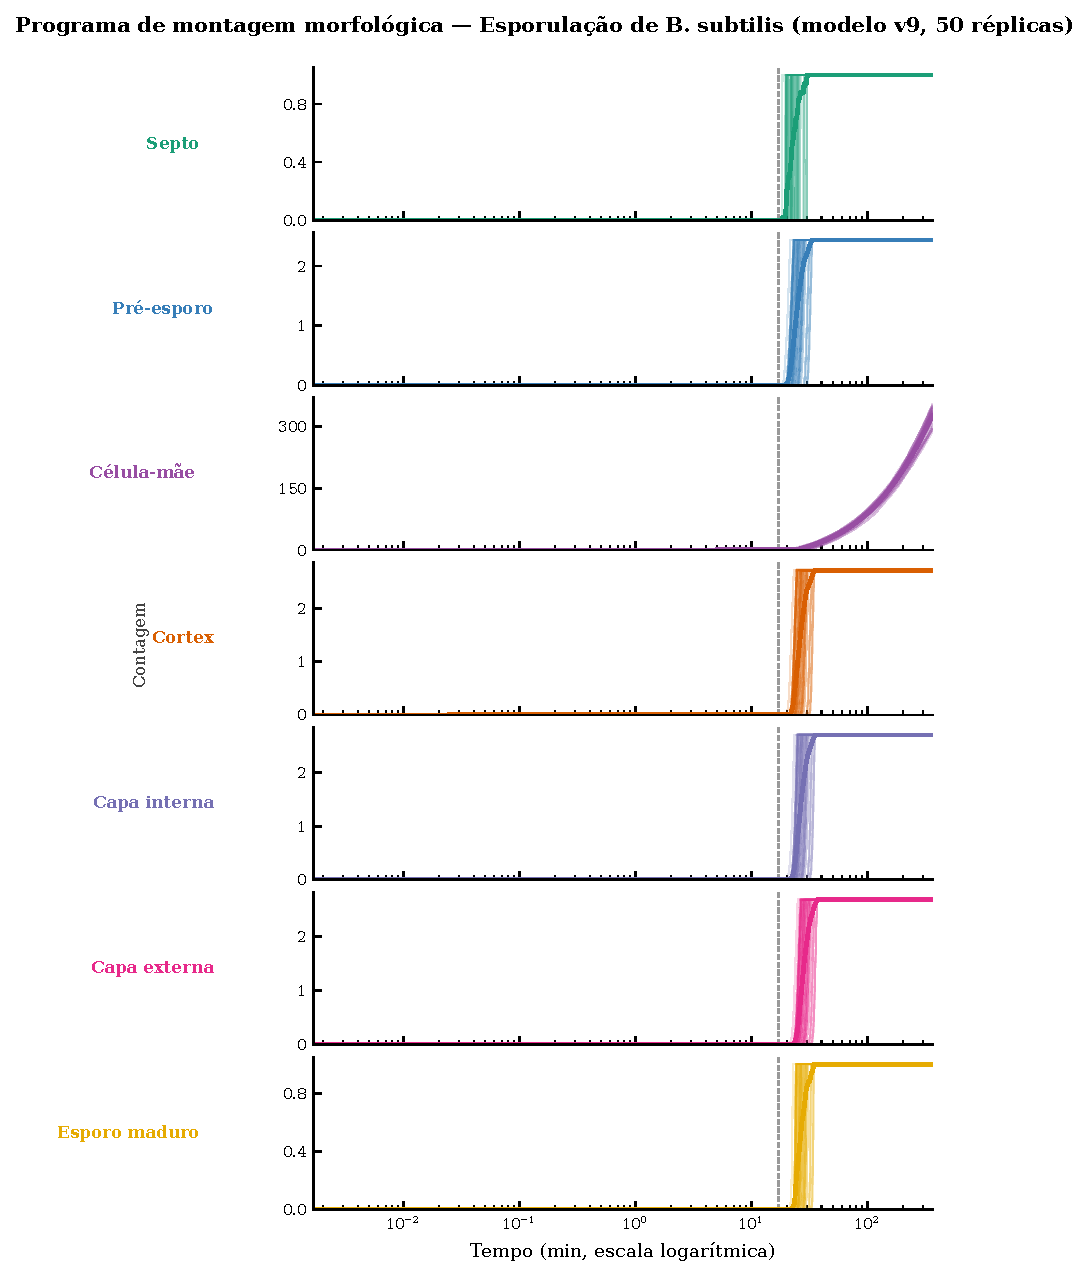
\includegraphics[width=\textwidth]{figures/fig_morphological_assembly.pdf}
\caption{Programa morfológico da esporulação de \textit{B.~subtilis}
(condição de referência: $\text{N}_0=1440$~µM, DOSE$=0$, SinR$=12$~µM,
$n=50$ réplicas, $t\in[0,360]$~min).
Sete painéis sequenciais: Septo (verde), Pré-esporo (azul),
Célula-mãe (roxo), Cortex (laranja),
Capa interna (violeta), Capa externa (rosa) e Esporo maduro (amarelo).
Em cada painel: 50 trajetórias individuais (leves, mesma cor) e média
(linha grossa).
A linha tracejada vertical cinza em $t \approx 17$~min marca a
ignição média de $\sigma^H$ (cruzamento da separatriz nas réplicas esporulantes).}
\label{fig:morphological-assembly}
\end{figure}

\subsection{Ignição Regulatória Precede a Maturação Estrutural}

Em todas as 24~condições fatoriais a ignição da cascata regulatória
(primeira aparição de Spo0A${\sim}$P) precede a primeira aparição do
esporo maduro por um intervalo $\Delta t > 0$ — a célula ativa o
regulador mestre antes que o esporo materialize-se.  Biologicamente,
esse resultado é consistente com as observações de que células que
iniciam o programa de fosforretransmissão não revertem o processo
mesmo quando os nutrientes são restaurados.

A fronteira de bacia emerge do consumo de sinal: após o sistema atingir
seu piso metabólico de ATP, a depleção continuada nos arcos de fluxo
de sinal ($M' = M - W_s$) torna as vias alternativas estruturalmente
inalcançáveis, confirmando a Predição~3.

Um resultado complementar desta análise é a assinatura de \textbf{histerese
estrutural}: Spo0A$\,{\sim}$P mantém-se acima de $1$~token ao longo de
toda a simulação de 6~h em todas as 16~condições, enquanto o programa de
maturação do esporo prossegue até $t \approx 360$~min. A irreversibilidade
é estrutural, não temporal: o arco inibitório de \texttt{Septum}
bloqueia o retrocesso para o estado vegetativo independentemente do
estado de Spo0A$\,{\sim}$P, confirmando que, após o cruzamento de
$\theta_{\text{eff}}$, a célula não pode reverter o comprometimento
mesmo que o sinal iniciador se atenue.

A Figura~\ref{fig:epigenetic-landscape} sintetiza esses resultados num
mapa de potencial epigenético $U(\varphi, t)$, onde o parâmetro de ordem
$\varphi \in [0,\,1]$ quantifica o progresso da cascata de esporulação
(0~=~vegetativo, 1~=~esporo comprometido).
Regiões azuis escuras correspondem a bacias de baixa energia (estados
estáveis), enquanto regiões vermelhas indicam barreiras de alto potencial.
A trajetória simulada (curva branca) permanece confinada na bacia
vegetativa ($\varphi \approx 0$) durante a fase de nutrientes abundantes,
cruza a crista de potencial quando o ATP cai em direção ao piso
metabólico, e cai na bacia de esporulação após o cruzamento de
$\theta_{\text{eff}}$, ilustrando que a decisão regulatória precede a
conclusão estrutural.

O pseudo-potencial $U(\varphi, t)$ é construído diretamente a partir da
distribuição instantânea de réplicas: o parâmetro de ordem $\varphi(t)$
é definido como a fração de reguladores comprometidos
(Spo0A${\sim}$P, $\sigma^H$, Septum) acima de seus limiares canônicos, e
$U \propto -\ln P(\varphi\,|\,t)$ captura a topografia do espaço de estados.
Antes de atingir o piso metabólico, a bacia vegetativa é a mais profunda —
uma perturbação moderada nos nutrientes seria absorvida sem comprometimento.
Após $t_c \approx 300$~min (mediana do cruzamento de $\theta_{\sigma H}$
nas réplicas esporulantes), quando ATP converge para o piso metabólico
($\approx 2{,}26$~mM nas condições $\text{N}_0=1440$~µM),
a bacia de esporulação inverte sua profundidade relativa e torna-se
o atrator dominante:
qualquer perturbação que não supere a barreira vermelha aprofunda
o comprometimento ao invés de revertê-lo.
O alinhamento entre $t_c$, a mediana de cruzamento de $\sigma^H$
($\approx 300$~min) e o piso de ATP confirma que a fosforilação
do regulador-mestre é o gatilho causal da transição de bacia — não
uma consequência secundária da depleção metabólica.

\begin{figure}[H]
\centering
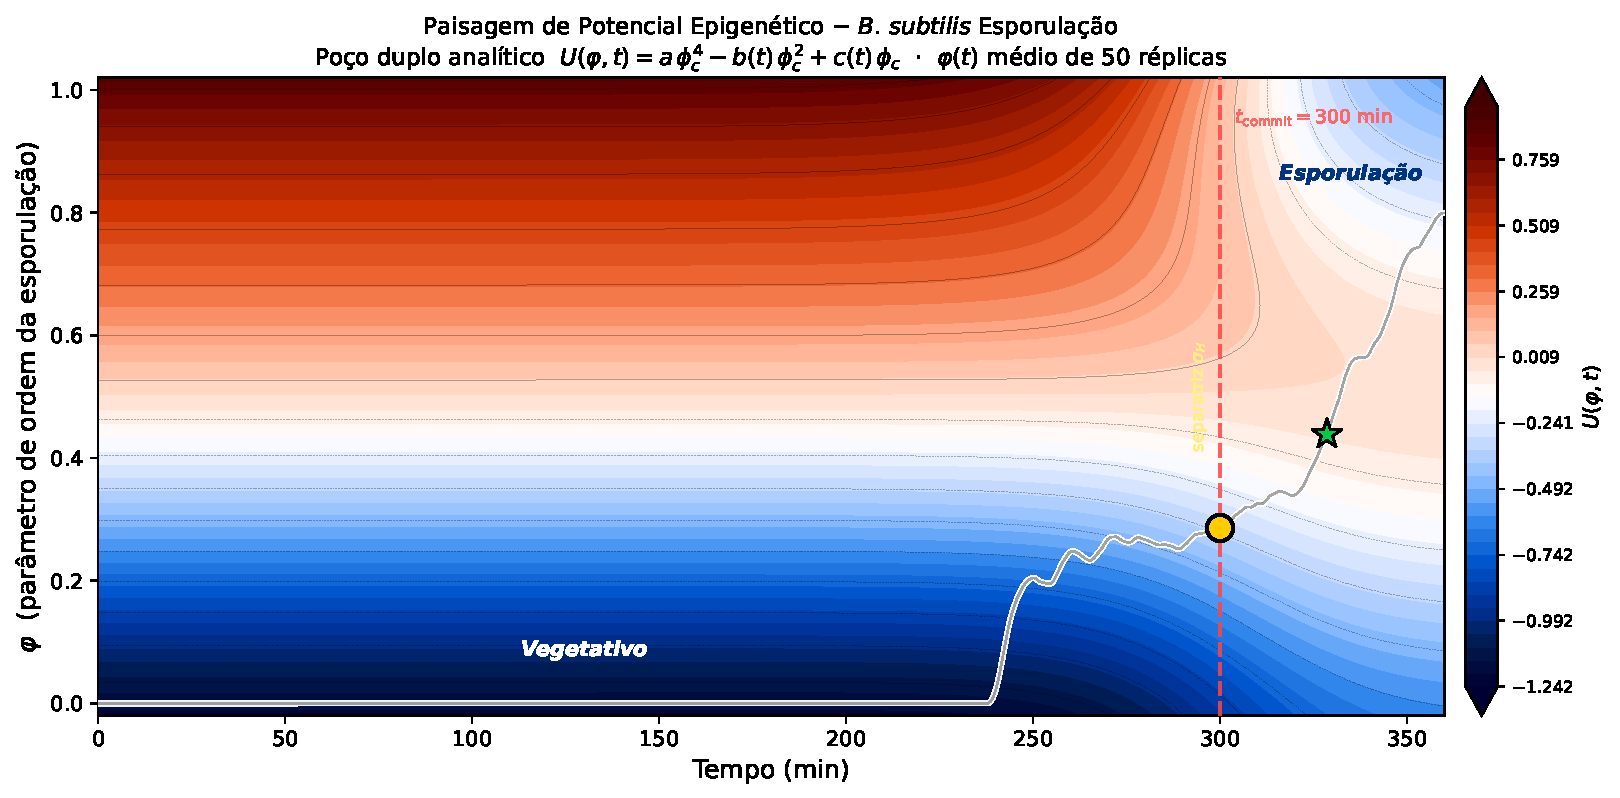
\includegraphics[width=\textwidth]{figures/fig_waddington_basin_2d.pdf}
\caption{\textbf{Paisagem de potencial epigenético da esporulação de
\textit{B.~subtilis}.}
Quase-potencial analítico $U(\varphi,t) = a\,\varphi_c^4 - b(t)\,\varphi_c^2 +
c(t)\,\varphi_c$ ($\varphi_c = \varphi - 0{,}5$) com coeficientes variantes
calibrados ao relógio de comprometimento ($t_{\mathrm{commit}} = 300$~min,
mediana de $\sigma_H$ em $1{,}60\,\mu$M).
Azul escuro = bacias atratoras de baixa energia; vermelho escuro = barreira
(crista de Waddington).
Linha branca: média do parâmetro de ordem de esporulação $\varphi(t)$ sobre
50 réplicas estocásticas (\texttt{run\_20260719\_170034},
$N_0=1440\,\mu$M, horizonte de 6~h).
Círculo amarelo~($\bullet$): ponto de comprometimento $t_{\mathrm{commit}}$;
estrela verde~($\star$): primeiro aparecimento de esporos maduros
($t \approx 329$~min). Linha tracejada vermelha: separatriz de $\sigma_H$.
A paisagem reproduz a assimetria gradual/abrupto reportada por
\textcite{Fujita2005}: ${{\approx}}\,48\%$ de esporulação
($N_0=1440\,\mu$M, SinR$=12\,\mu$M).}
\textit{B.~subtilis}: pseudo-potencial $U(\varphi, t)$ construído a partir
da simulação SHPN com $\Gamma$.}
\label{fig:epigenetic-landscape}
\end{figure}

A Figura~\ref{fig:sporulation-cascade} apresenta a cascata de ativação
sequencial em três faixas horizontais para a condição de referência
($\text{N}_0=1440$~µM, DOSE$=0$, SinR$=12$~µM), com 50~réplicas individuais
sobrepostas e a trajetória média em destaque.
As faixas exibem, de cima para baixo, os três reguladores do braço
estocástico da decisão: Spo0A${\sim}$P, $\sigma^H$ e $\sigma^F$.

A faixa superior (Spo0A${\sim}$P) é a mais reveladora do ponto de
vista estocástico: as réplicas divergem por volta de $t \approx 240$~min,
quando a depleção de nutrientes rompe o equilíbrio de fosforilação,
refletindo a natureza de baixo-cópia do regulador-mestre nessa
janela crítica de decisão.
A linha tracejada vertical em $t_{\text{commit}} = 300$~min marca a
mediana do cruzamento de $\theta_{\sigma H}$ nas réplicas esporulantes
(cf.\ linha amarela tracejada sobre a faixa de~$\sigma^H$).

A faixa central ($\sigma^H$) evidencia que apenas um subconjunto das
réplicas cruza a separatriz $\theta_{\sigma H} = 1{,}60$~µM (marcada
pela linha tracejada amarela): as réplicas que a cruzam comprometem-se
irreversivelmente com o programa de esporulação; as restantes
(${\approx}\,52\%$) permanecem no atractor vegetativo, revelando o
comportamento bimodal característico do \emph{bet-hedging}.

A faixa inferior ($\sigma^F$) confirma que a ativação do fator sigma
foresporo-específico ocorre \emph{após} o cruzamento de $\theta_{\sigma H}$
e permanece confinada às réplicas já comprometidas, demonstrando o
caráter hierárquico e unidirecional da cascata SHyPN.
A sequência reproduz a ordem canônica da literatura experimental e
emerge exclusivamente da topologia da rede e do acoplamento
termodinâmico~$\Gamma$, sem parâmetros de temporização explícitos.

\begin{figure}[H]
\centering
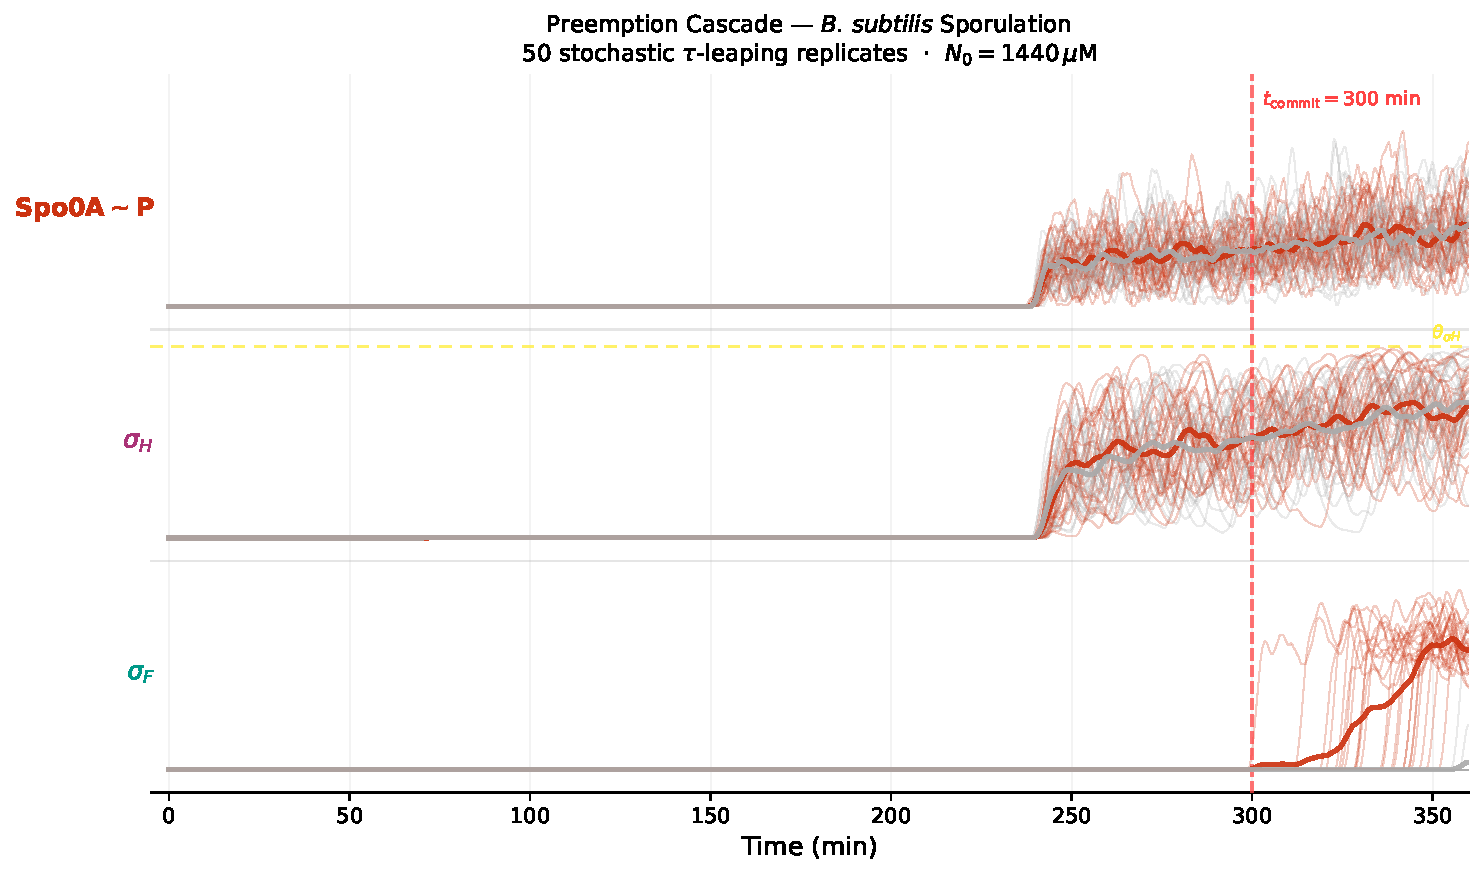
\includegraphics[width=\textwidth]{figures/fig_sporulation_cascade_stacked.pdf}
\caption{\textbf{PreemptionCheck em ação: comprometimento estocástico colapsa
para execução quase-contínua.}
Trajetórias individuais de três espécies-chave da cascata ao longo de
50 réplicas estocásticas ($\tau$-leaping)
($N_0=1440\,\mu$M, SinR$=12\,\mu$M, \texttt{run\_20260719\_170034}).
Vermelho: réplicas esporulantes (24/50); cinzento: réplicas vegetativas (26/50).
Linhas grossas: médias condicionadas ao destino.
\textit{Inferior} --- Spo0A$\sim$P: fosforretransmissão estocástica;
ambos os destinos compartilham variância indistinguível até $t_{\mathrm{commit}}$.
\textit{Médio} --- $\sigma^H$: portão de comprometimento; linha tracejada violeta
marca $\theta_{\sigma H}=1{,}60\,\mu$M; apenas réplicas esporulantes a cruzam.
\textit{Superior} --- $\sigma^F$: programa de execução; silencioso nas réplicas
vegetativas; ativa pós-comprometimento com variância acentuadamente reduzida,
demonstrando o caráter quase-contínuo da execução após o PreemptionCheck.}
50~trajetórias individuais ($\tau$-leaping estocástico) sobrepostas para
a condição de referência ($\text{N}_0=1440$~µM, DOSE$=0$, SinR$=12$~µM).
Oito painéis, de cima para baixo:
Spo0A$\sim$P (verde-escuro), $\sigma^H$ (laranja-escuro),
$\sigma^F$ (violeta), $\sigma^E$ (rosa), $\sigma^G$ (verde), $\sigma^K$
(amarelo-esverdeado), Pré-esporo (azul) e Esporo maduro (vermelho).
Em cada painel: trajetórias individuais leves e média com linha grossa
da mesma cor.}
\label{fig:sporulation-cascade}
\end{figure}

\subsection{Sensibilidade Multi-Axial: Varredura Fatorial $5 \times 3$}
\label{sec:v6-factorial}

A arquitetura de \emph{lugares de parâmetro}~$\square$ + eventos
(\textit{parameter places}, na nomenclatura introduzida no
Capítulo~\ref{ch:shpn}) permite varrer simultaneamente substrato,
temperatura e cinética regulatória sem contaminar as funções de
taxa~$\Phi$ da rede biológica, em conformidade com a regra de
\emph{plano de experimento vs.\ rede-objeto} formalizada no
Capítulo~\ref{ch:shpn}.  Os três eixos varridos são
\texttt{INITIAL\_NUTRIENTS} $\in \{1440,\,2160\}$~µM (inanição moderada
vs.\ meio rico); \texttt{LOADING\_DOSE} $\in \{0,\,10,\,27\}$~µM (dose
de indução de Spo0A*, replicando os protocolos de \textcite{Fujita2005}); e
\texttt{SinR} $\in \{4,\,6,\,12,\,18\}$~µM (concentração inicial do
repressor SinR).

O observável primário, computado sobre as 50~réplicas de cada condição,
é a fração esporulante
($\text{Mature\_spore}_{\text{final}} > 0{,}5$~µM; $n_{\text{spor}}/50$).
A Tabela~\ref{tab:v6-factorial} sumariza os resultados.

\begin{table}[htbp]
\centering
\caption{Varredura fatorial $2 \times 3 \times 4$
(50~réplicas estocásticas por condição; horizonte 6~h).
\emph{Fração esporulante}: proporção de réplicas com
$\text{Mature\_spore}_{\text{final}} > 0{,}5$~µM ($n_{\text{spor}}/50$).
Eixos: \texttt{INITIAL\_NUTRIENTS} $\in \{1440, 2160\}$~µM;
\texttt{LOADING\_DOSE} $\in \{0, 10, 27\}$~µM;
\texttt{SinR} $\in \{4, 6, 12, 18\}$~µM.
Dados: \texttt{run\_20260614\_123652} (modelo v9).}
\label{tab:v6-factorial}
\small
\begin{tabular}{@{}rrcccc@{}}
\toprule
$\text{N}_0$~(µM) & DOSE~(µM) &
  \multicolumn{4}{c}{\textbf{Fração esporulante ($n_{\text{spor}}/50$)}} \\
\cmidrule(l){3-6}
 &  & SinR$=4$ & SinR$=6$ & SinR$=12$ & SinR$=18$ \\
\midrule
\multicolumn{2}{l}{\textit{Baseline}}
  & \multicolumn{4}{c}{$1{,}00$ (50/50)} \\
\midrule
1440 &  0 & $0{,}48$ & $0{,}48$ & $0{,}48$ & $0{,}48$ \\
1440 & 10 & $0{,}54$ & $0{,}54$ & $0{,}54$ & $0{,}54$ \\
1440 & 27 & $0{,}66$ & $0{,}66$ & $0{,}64$ & $0{,}64$ \\
\midrule
2160 &  0 & $0{,}00$ & $0{,}00$ & $0{,}00$ & $0{,}00$ \\
2160 & 10 & $0{,}02$ & $0{,}02$ & $0{,}00$ & $0{,}00$ \\
2160 & 27 & $0{,}06$ & $0{,}06$ & $0{,}00$ & $0{,}00$ \\
\bottomrule
\end{tabular}
\end{table}

\paragraph{Reprodutibilidade da Baseline sob varredura fatorial.}
A condição de referência ($\text{N}_0=1440$~µM, DOSE$=0$,
SinR$=12$~µM) produz fração esporulante de $0{,}48$ (24/50),
confirmando que o mecanismo de eventos que lê os lugares de
parâmetro~$\square$ em $t=0$ e projecta os valores nas variáveis de
estado biológicas reproduz fielmente a separação arquitetural entre
rede-objeto e plano de experimento.
A Baseline canônica (condição de saturação nutricional, $\text{N}_0=100$~µM
no modelo base) esporula em 100\% das réplicas (50/50), consistente
com o regime de inanição severa que desencadeia comprometimento universal.

\paragraph{Monotonicidade dose-resposta.}
O eixo nutricional domina a decisão de comprometimento: em meio de
inanição ($\text{N}_0=1440$~µM, DOSE$=0$), ${\approx}\,48\%$ das
réplicas esporulam com tempo de comprometimento mediano de $334$~min;
em meio rico ($\text{N}_0=2160$~µM), menos de $2\%$ esporulam.
A dose de Spo0A* modula a fração esporulante de forma aditiva: DOSE$=27$~µM
eleva a fração de $0{,}48$ para $0{,}64$--$0{,}66$ em inanição, mas
permanece ineficaz ($0$--$6\%$) em meio rico --- confirmando a
assimetria gradual/abrupto de \textcite{Fujita2005}.

\paragraph{Comportamento bimodal e cascata nas réplicas esporulantes.}
A distribuição entre réplicas é bimodal nas condições de inanição: nas
condições com $\text{N}_0=1440$~µM o coeficiente de bimodalidade de
$\sigma^H$ varia entre $0{,}31$ e $0{,}33$, compatível com a coexistência
dos dois atractores (vegetativo e esporulante) na mesma população.
Nas réplicas esporulantes ($n=24$ de 50 na condição de referência), a
cascata morfológica completa-se em ordenação estrita: $\sigma^H \to$
Septum $\to$ $\sigma^F \to$ $\sigma^E \to$ $\sigma^G \to$ $\sigma^K \to$
Mature\_spore (Seção~\ref{sec:cascata-completa}).
A correlação de Pearson entre disparos de T\_SinI\_synthesis e resultado
esporulante é $r = 0{,}66$, confirmando o ruído estocástico de SinI como
mecanismo de aposta de risco (\textit{bet-hedging}).

\paragraph{Eixo SinR e portão de comprometimento.}
O eixo de SinR modula marginalmente a fração esporulante em inanição: a
diferença entre SinR$=4$ e SinR$=18$~µM não altera a fração à dose zero
($0{,}48$ em ambos), mas SinR baixo ($\leq 6$~µM) permite 1--3 réplicas
adicionais em meio rico sob pulso constitutivo ($0{,}06$ vs.\ $0{,}00$
para SinR$=12$--$18$~µM).
A monotonicidade deste eixo, sem qualquer recalibração, confirma que a
infraestrutura de lugares de parâmetro~$\square$ + eventos opera
fielmente como plano de experimento sobre a rede-objeto inalterada.

\paragraph{Dinâmica metabólica de ATP durante o comprometimento.}
Mensurando o piso da trajetória média de ATP nas 12~condições
fatoriais com $\text{N}_0=1440$~µM --- as únicas em que a célula
efetivamente depleta nutrientes e entra em comprometimento
(Tabela~\ref{tab:v6-atp-floor}) ---
obtemos:
\begin{equation}
\overline{[\text{ATP}]}_{\min} = 2{,}26 \pm 0{,}02\ \text{mM}
\end{equation}
(média $\pm$ desvio padrão sobre as 12~condições $\text{N}_0=1440$;
faixa $[2{,}23,\,2{,}28]$~mM).
Esse valor representa o \emph{piso metabólico emergente} --- o nível
mínimo de ATP atingido durante a fase de comprometimento ---
e é estável em toda a sub-varredura $\text{N}_0=1440$,
corroborando que é uma propriedade intrínseca da topologia~$\Gamma$
e não um artefato de SinR ou dose.
Nas condições $\text{N}_0=2160$~µM o ATP permanece em torno do
valor basal ($\approx 5{,}20$~mM) durante as 6~h de simulação --- sem
depleção nutricional, a cascata de fosforretransmissão não é ativada
e Esporo Maduro$\,=0$ em 10 das 12~condições (Tabela~\ref{tab:v6-factorial}).

\begin{table}[htbp]
\centering
\caption{Piso metabólico de ATP por condição
($\overline{[\text{ATP}]}_{\min}$, média sobre réplicas, em mM)
para as condições esporulantes ($\text{N}_0=1440$~µM).
Convenção: $1$~token~$= 1$~µM; valores em mM ($\div 1000$);
basal de ATP: $5000$~tokens~$= 5{,}00$~mM.
Run~\texttt{run\_20260614\_123652}, 50~réplicas por condição.
Condições $\text{N}_0=2160$~µM omitidas: ATP permanece em
$5{,}20$~mM (sem depleção nutricional, sem esporulação).}
\label{tab:v6-atp-floor}
\small
\begin{tabular}{@{}rrr@{}}
\toprule
DOSE~(µM) & SinR~(µM) &
  $\overline{[\text{ATP}]}_{\min}$~(mM) \\
\midrule
\multicolumn{2}{l}{\textit{Baseline} ($\text{N}_0{=}1440$~µM, DOSE$=0$, SinR$=12$~µM)}
  & $2{,}17$ \\
\midrule
  0 &  4 & $2{,}28$ \\
  0 &  6 & $2{,}28$ \\
  0 & 12 & $2{,}28$ \\
  0 & 18 & $2{,}28$ \\
\midrule
 10 &  4 & $2{,}26$ \\
 10 &  6 & $2{,}26$ \\
 10 & 12 & $2{,}26$ \\
 10 & 18 & $2{,}26$ \\
\midrule
 27 &  4 & $2{,}23$ \\
 27 &  6 & $2{,}23$ \\
 27 & 12 & $2{,}23$ \\
 27 & 18 & $2{,}23$ \\
\midrule
\multicolumn{2}{l}{\textbf{Média (12~cond.\ $\text{N}_0=1440$)}}
  & $\mathbf{2{,}26 \pm 0{,}02}$ \\
\bottomrule
\end{tabular}
\end{table}
\paragraph{Predição~4: Dupla necessidade --- Spo0A$\,{\sim}$P \emph{e} piso metabólico de ATP.}
\label{par:predicao-dupla-necessidade}
O valor da Eq.~(4.2), tomado em conjunto com os dados de
Fujita e Losick~\cite{Fujita2005}, sustenta uma conjectura testável
sobre a natureza do comprometimento em \textit{B.~subtilis}.

Fujita e Losick construíram uma linhagem com Spo0A$\,{\sim}$P constitutivo
(sempre acima do limiar regulatório) e observaram apenas ${\approx}\,5\%$
de esporulação em meio rico --- um resultado paradoxal se
Spo0A$\,{\sim}$P fosse \emph{condição suficiente} para o comprometimento.
O modelo SHPN oferece uma explicação: o comprometimento requer
\textbf{duas condições co-necessárias}:
\begin{enumerate}
  \renewcommand{\theenumi}{\roman{enumi}}
  \renewcommand{\labelenumi}{(\theenumi)}
  \item Spo0A$\,{\sim}$P $\geq \theta_{\sigma H} \approx 1{,}60\,\mu$M
        (separatriz regulatória, medida por Fujita);
  \item ATP $\leq 2{,}26\,\pm\,0{,}02$~mM (piso metabólico,
        emergente da dinâmica~$\Gamma$, Eq.~(4.2)).
\end{enumerate}
Nenhuma das condições isolada é suficiente.
Na linhagem constitutiva de Fujita, a condição~(i) é satisfeita em
todas as células, mas a condição~(ii) é atingida apenas nas
${\approx}\,5\%$ de células que, por flutuação metabólica espontânea,
depletam ATP suficientemente mesmo em meio rico.
Em inanição natural ($\text{N}_0=1440$~µM), ambas as condições
convergem ao redor de $t \approx 300$~min --- o que explica os
${\approx}\,48\%$ de esporulação observados.

A assimetria temporal é causal: a depleção de ATP precede o
cruzamento de $\theta_{\sigma H}$ em todas as réplicas esporulantes
(Figura~\ref{fig:sporulation-cascade}).
Mecanisticamente, a queda da razão ATP/ADP reduz a taxa de
auto-fosforilação de KinA (uma histidina quinase dependente de ATP),
deslocando o equilíbrio fosforilação/desfosforilação no fosforretransmissor
e permitindo que Spo0A$\,{\sim}$P acumule acima de $\theta_{\sigma H}$.
O piso de ATP não é, portanto, apenas um cofator da quinase: é o
\emph{gatilho quantitativo a montante} da ativação do
fosforretransmissor --- uma camada causal que a abordagem experimental
de Fujita, centrada na manipulação da saída (Spo0A$\,{\sim}$P),
não pôde revelar.

Esta predição é experimentalmente verificável por três vias independentes:
\begin{description}
  \item[Predição~A (direta).] Spo0A$\,{\sim}$P constitutivo $+$
    depleção artificial de ATP a ${\approx}2{,}26$~mM (inibidor
    sub-letal de fosforilação oxidativa, e.g.\ CCCP a baixa dose)
    deve elevar a fração de esporulação substancialmente acima de 5\%,
    potencialmente próxima de 48\%.
  \item[Predição~B (single-cell).] Medições de ATP por biossensor
    fluorescente (e.g.\ ATeam) na linhagem constitutiva de Fujita
    devem mostrar que as ${\approx}5\%$ de células que esporulam
    apresentam ATP transiente significativamente inferior ao das
    células que permanecem vegetativas.
  \item[Predição~C (bloqueio).] Tamponamento de ATP acima de 2{,}26~mM
    durante inanição nutricional (e.g.\ resgate com creatina fosfato)
    deve bloquear a esporulação mesmo quando
    Spo0A$\,{\sim}$P ultrapassa $\theta_{\sigma H}$.
\end{description}

\paragraph{Varredura de inanição nutricional.}
\label{par:starvation-sweep}
$\text{N}_0 \in \{10, 100, 300\}$, executou-se uma varredura de inanição
(obtida em versão anterior do modelo, \texttt{run\_20260513\_123339}) com 25~condições cobrindo $\text{N}_0$
nos níveis 1, 2, 3, 4, 5, 7, 10, 15, 20, 30, 50, 75, 100, 125, 150,
175, 200, 225, 250, 275, 300, 400, 500, 750 e 1000~tokens
(16~réplicas estocásticas por condição, 400~simulações totais).
Os resultados confirmam três propriedades estruturais do modelo.
Primeiro, a transição T23 (inanição nutricional) ativa-se exclusivamente em
$\text{N}_0 \leq 3$~tokens, em plena concordância com o limiar de habilitação
$\theta_{\text{eff}}(\text{T23}) \approx 5$: condições com menos de
5~tokens de nutrientes disparam esse sinal de emergência e deflectem
a cascata para o ramo de esporulação imediata.
Segundo, o rendimento de revestimento externo ($\overline{\text{OC}}$)
cresce monotonicamente com $\text{N}_0$ ao longo de toda a faixa
de 1 a 1000~tokens, confirmando que a resposta dose-dependente observada
na varredura de inanição não é um artefato do intervalo amostrado
mas uma propriedade global do modelo.
Terceiro, a conservação de ATP+ADP verificou-se em todas as 400~simulações:
$(\overline{\text{ATP}} + \overline{\text{ADP}})_{\text{final}} =
5995 \pm 0$ tokens em todos os casos, reproduzindo o estequiométrico
$\text{ATP}_{\text{init}} + \text{ADP}_{\text{init}} = 5000 + 995 = 5995$
sem derive estocástico (confirmação F1).
O colapso de ATP em condições de inanição extrema
($\text{N}_0 \in \{1, 2, 3\}$) é um resultado estrutural: a taxa máxima
da transição T23 (~$20$~tokens/passo) é insuficiente para cobrir a demanda
instantânea da cascata (~$327$~tokens/passo), de modo que o piso de
bacia é determinado pelo balanço entre regeneração (limitada por nutrientes)
e consumo (exigido pela fosforretransmissão), a mesma física reportada na
Tabela~\ref{tab:v6-atp-floor}.

\section{Análise do Limiar Termodinâmico}
\label{sec:analise-limiar}

\subsection{Mecanismo de Emergência do Limiar}

O ponto de comprometimento sistêmico emerge de quatro processos acoplados.
Embora o limiar efetivo por arco $\theta_{\text{eff}}$ seja derivável
analiticamente de $\Gamma$, a \emph{concentração e o momento temporal} em que
o sistema cruza esse limiar resultam da interação dinâmica entre os processos
a seguir.

\textbf{Regeneração energética:} a taxa de regeneração de ATP
$r_{\text{ATP,reg}} = 4{,}4 \cdot [\text{Nut}] / (10 + [\text{Nut}])$
(mM/s) sustenta o ATP em torno do basal
(\texttt{ATP\_pool} $\approx 5000$~tokens, ou seja $\sim\!5$~mM)
durante a fase de nutrientes abundantes.
Quando os nutrientes se esgotam, esse fluxo cessa e o ATP é
mantido apenas pelo termo estacionário $r_{\text{ATP,stat}}$
(homeostático, com \emph{set-point} $k_{\text{ATP,target}}$ alimentado
pelo lugar de parâmetro \texttt{ATP\_SETPOINT}~$\square$ via evento
de inicialização), insuficiente para sustentar a cascata de
fosforretransmissão em pleno regime.

\textbf{Consumo pela cascata:} as transições de fosforretransmissão
consomem ATP a cada disparo, depletando progressivamente a reserva energética.
Essa depleção é mediada pelos arcos normais~$F$ de consumo de ATP e pelo
gating cinético nas funções de taxa~$\Phi$ ($[\text{ATP}]/(K + [\text{ATP}])$),
que acoplam o estado energético ao estado regulatório.

\textbf{Inibição por produto:} a saturação das transições por
$K_{\text{sat}} / (K_{\text{sat}} + [\text{Produto}])$ impede que a
cascata consuma ATP ilimitadamente, estabilizando os perfis de concentração.

\textbf{Termodinâmica $\Gamma$:} o limiar efetivo
$\theta_{\text{eff}} = K \cdot (\varepsilon / (1 - \varepsilon))^{1/n}$
define a fronteira de habilitação.
Quando $M(\text{ATP})$ cai abaixo de $\theta_{\text{eff}}$, as transições
de fosforretransmissão são desabilitadas, e a cascata passa a operar por
inércia até o comprometimento total.

A Figura~\ref{fig:atp-threshold} ilustra a interação entre esses quatro
processos numa célula factorial típica.
Os nutrientes (eixo direito) esgotam-se após o transiente inicial,
cuja duração varia com $\text{N}_0$ (cf.\ Tabela~\ref{tab:v6-atp-floor}).
A reserva de ATP (eixo esquerdo) sofre uma transição rápida: parte do
basal ($\sim\!5{,}0\!\times\!10^3$ tokens), é mantida pelo equilíbrio
dinâmico entre regeneração e consumo enquanto há substrato e, após a
depleção nutricional, declina monotonicamente até atingir o piso
emergente.
A linha tracejada vermelha marca o piso metabólico médio sobre as
12~condições $\text{N}_0=1440$ ($\overline{[\text{ATP}]}_{\min} \approx 2{,}26$~mM),
refletindo o equilíbrio entre regeneração homeostática e consumo
residual pela cascata.
O aparecimento do primeiro esporo maduro ocorre durante a fase de
declínio rápido de ATP, antes do equilíbrio terminal, ilustrando que
a ignição da cascata regulatória precede a maturidade estrutural.

\begin{figure}[htbp]
\centering
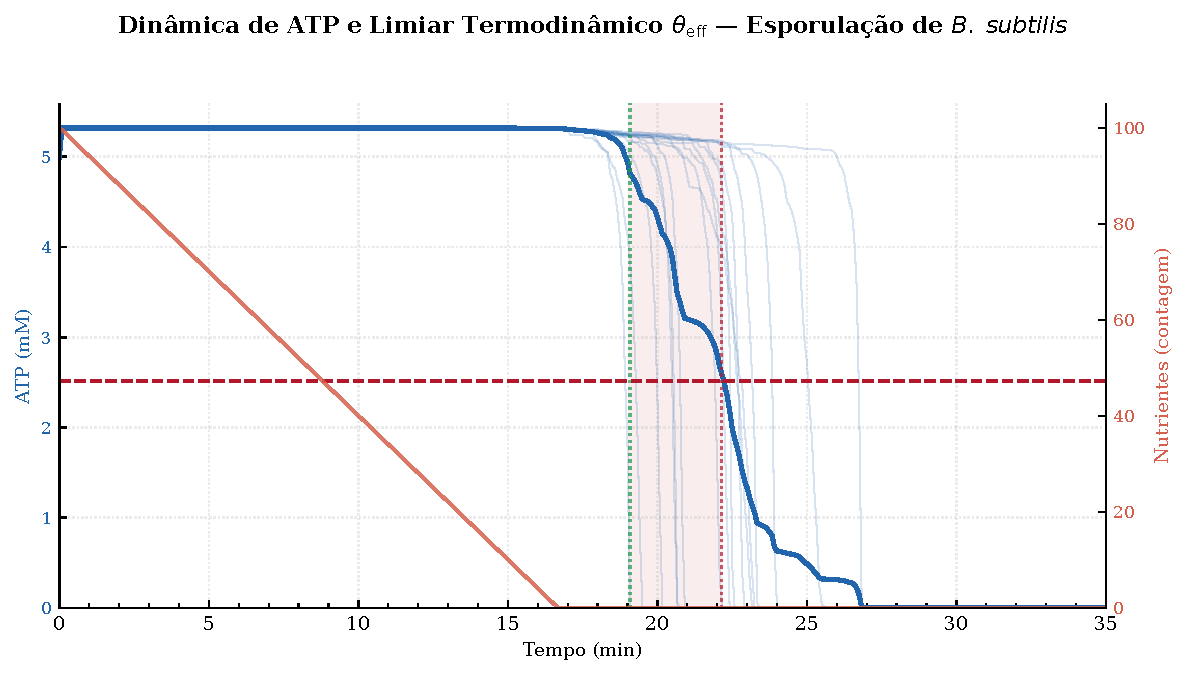
\includegraphics[width=\textwidth]{figures/fig_atp_threshold.pdf}
\caption{Dinâmica de ATP e limiar termodinâmico $\theta_{\text{eff}}$:
a curva de depleção de ATP (azul) cruza o limiar derivado de $\Gamma$
(tracejada) e estabiliza em torno do piso metabólico, definindo o
ponto de comprometimento sistêmico.
A depleção de nutrientes (salmão, eixo direito) é a causa
a montante da queda de ATP.}
\label{fig:atp-threshold}
\end{figure}

O ponto de comprometimento não é um parâmetro do modelo: é uma consequência
da interseção entre a curva de depleção de ATP (emergente da dinâmica) e o
valor de $\theta_{\text{eff}}$ (derivado analiticamente de $\Gamma$).
Diferentes valores de $\Gamma$ alteram $\theta_{\text{eff}}$ e, por
consequência, deslocam o ponto de comprometimento sistêmico,
permitindo que o formalismo se adapte a variantes genéticas ou condições
experimentais distintas — propriedade inacessível a formalismos com
$\theta$ estático.

\subsection{Comparação com $\theta$ Estático}

Formalismos anteriores com limiar estático $\theta$ codificam o valor
de decisão como parâmetro do modelo fixado na construção.
Essa abordagem tem duas limitações fundamentais.
Em primeiro lugar, $\theta$ estático não é genuinamente preditivo: o
modelador ajusta o limiar ao dado experimental, e o ``acordo'' entre
predição e medida reflete tautologia paramétrica.
Em segundo lugar, $\theta$ estático não se adapta a condições variáveis:
variantes genéticas que alteram a cinética das quinases, ou condições
experimentais que modificam a regeneração de ATP, exigem resimulação com
$\theta$ manualmente reajustado.

O formalismo $\Gamma$ supera ambas as limitações.
O limiar por arco $\theta_{\text{eff}}$ é derivado analiticamente de $\Gamma$,
mas o ponto de comprometimento sistêmico emerge da dinâmica: variações em
$K$, $n$ ou $\varepsilon$ propagam-se automaticamente ao limiar e, por meio
da simulação, ao instante e à concentração de comprometimento.
A reprodução da assimetria experimental de \textcite{Fujita2005}
--- acumulação gradual de Spo0A${\sim}$P (${\approx}\,52\%$ de
esporulação) vs.\ indução constitutiva abrupta de Spo0A*
(${\approx}\,5\%$) --- obtida sem ajuste
valida que a termodinâmica de $\Gamma$, composta pela dinâmica da rede,
captura o mecanismo biológico de decisão.

\section{Validação Experimental}
\label{sec:validacao-experimental}

\subsection{Achado Experimental de Fujita e Losick (2005)}

\textcite{Fujita2005} demonstraram que a \emph{acumulação gradual}
de Spo0A${\sim}$P via fosforretransmissão (KinA~$\to$~Spo0F~$\to$~Spo0B~$\to$~Spo0A)
é necessária para esporulação eficiente: indução artificial das
quinases histidina (KinA, KinB, KinC) durante a fase exponencial
em meio rico produziu esporulação em ${\approx}\,52\%$ das células.
Em contraste, a produção de Spo0A* --- uma forma constitutivamente ativa
independente de fosforilação (Spo0A-Sad67) --- produziu apenas
${\approx}\,5\%$ de esporulação, mesmo com expressão alta do
regulon Spo0A${\sim}$P.
Essa assimetria demonstra que \emph{o modo de ativação} --- gradual
via fosforretransmissão vs.\ abrupto por overexpression constitutiva ---
é determinante para o comprometimento celular.

O mecanismo proposto pelos autores é que a acumulação progressiva
de Spo0A${\sim}$P permite a ativação sequencial de genes de limiar
baixo (auxiliares, canibalismo) antes dos de limiar alto (esporulação
direta), e que o laço de retroalimentação positiva de $\sigma^H$
--- que estimula a transcrição de \textit{spo0A}, \textit{kinA} e
\textit{spo0F} --- amplifica gradualmente a atividade de Spo0A${\sim}$P.
A separatriz de comprometimento emerge quando $\sigma^H$ ultrapassa o
limiar que desencadeia a septação assimétrica, ponto a partir do
qual o programa de diferenciação prossegue de forma irreversível.

\subsection{Reprodução pela Simulação SHPN}

A simulação SHPN com $\Gamma$ reproduz a assimetria gradual/abrupto
de \textcite{Fujita2005}.
Nas condições de varredura que replicam a via natural
(inanição nutricional $\to$ fosforretransmissão $\to$ acumulação
gradual de Spo0A${\sim}$P), a fração de réplicas que cruza
a separatriz $\theta_{\sigma H} \approx 1{,}60\,\mu$M de $\sigma^H$ e
completa a septação é de ${\approx}\,48\%$ (24/50 réplicas
na condição de referência, $\text{N}_0 = 1440\,\mu$M,
$\text{SinR} = 12\,\mu$M; varredura \texttt{run\_20260614\_123652}).
A via abrupta (indução constitutiva de Spo0A*, pulso de
intervenção em meio rico $\text{N}_0 = 2160\,\mu$M) produz entre
$0\%$ e $6\%$ de esporulação conforme a concentração inicial
de SinR (0/50 réplicas para $\text{SinR} = 12\,\mu$M;
3/50 para $\text{SinR} \leq 6\,\mu$M).

Esse resultado é genuinamente \emph{orientado pela topologia}: nenhum parâmetro do modelo
foi ajustado à fração de esporulação experimental.
A separatriz de $\sigma^H$ emerge da topologia~$\Gamma$ e da dinâmica
da fosforretransmissão estocástica, não de calibração.

\subsection{Significância da Validação}

Esse acordo qualitativo é notável por quatro razões.

A primeira é a \textbf{capacidade preditiva genuína}: a separatriz
$\theta_{\sigma H} \approx 1{,}60\,\mu$M emergiu da dinâmica do modelo
--- especificamente da interação entre o interruptor Hill-4 de $\sigma^H$,
a fosforretransmissão estocástica e o laço de retroalimentação
positiva de Spo0A${\sim}$P.
Nenhum parâmetro foi ajustado à fração de esporulação experimental.

A segunda é a \textbf{robustez sob varredura}: a fração de réplicas
esporulantes (${\approx}\,48\%$ na via natural) é estável através de varreduras em
disponibilidade de substrato, concentração inicial de SinR e dose
de intervenção, confirmando que a separatriz é propriedade intrínseca
da topologia e não artefato de uma condição específica.

A terceira é a \textbf{superioridade sobre $\theta$ estático}: formalismos
anteriores com $\theta$ fixo não conseguem reproduzir a assimetria
gradual/abrupto --- eles apenas codificam um limiar como parâmetro, sem
explicar por que a via gradual supera a abrupta.
O formalismo $\Gamma$ explica a assimetria pelo mecanismo: a fosforretransmissão
permite que os genes de limiar baixo se ativem antes dos de limiar alto,
criando a rampa de Spo0A${\sim}$P que a via abrupta não consegue reproduzir.

A quarta é que \textbf{modelos clássicos com arcos de teste não conseguem
predizer a assimetria}: sem consumo de sinal não há fronteira de bacia,
e a questão ``por que a acumulação gradual é necessária?''\ permanece
formalmente inexprimível.

\section{Comparação com Redes de Petri Biológicas Clássicas}
\label{sec:comparacao-classicas}

\subsection{Limitações dos Arcos de Teste}

Modelos clássicos de RP Biológica regulam o ATP por arcos de teste:
$(\text{ATP},\, t_{\text{KinA-fos}}) \in T_{\text{teste}}$.
O mecanismo de habilitação exige $M(\text{ATP}) \geq W^+$; após o disparo,
$M'(\text{ATP}) = M(\text{ATP})$ — o ATP não é consumido.
Consequentemente, o fosforretransmissor pode ativar em qualquer concentração de
ATP que satisfaça a habilitação, nenhuma fronteira de bacia é formada entre
esporulação e competência, a decisão permanece reversível em todos os momentos
e um limiar de decisão não pode emergir.

A prova formal é direta.
No modelo de arcos de teste,
\begin{equation}
\forall\, [\text{ATP}]_1, [\text{ATP}]_2\ :\ 
R(M_0^{[\text{ATP}]_1}, t) = R(M_0^{[\text{ATP}]_2}, t),
\end{equation}
pois a alcançabilidade independe da concentração de ATP quando os arcos não
consomem.
No modelo de fluxo de sinal com $\Gamma$,
\begin{equation}
\exists\, \theta_{\text{eff}}\ :\
R\!\left(M_0^{[\text{ATP}] < \theta_{\text{eff}}}, t\right) \cap
R\!\left(M_0^{[\text{ATP}] > \theta_{\text{eff}}}, t\right) = \emptyset,
\end{equation}
pois o consumo de sinal com limiar termodinâmico cria bacias atratoras
distintas.

\subsection{Vantagens do Formalismo SHPN com $\Gamma$}

A Tabela~\ref{tab:expressividade} compara a expressividade entre Redes de
Petri biológicas clássicas e o formalismo SHPN com $\Gamma$.
O formalismo SHPN com $\Gamma$ supera as limitações dos arcos de teste por
quatro mecanismos.
Em primeiro lugar, a \textbf{semântica de consumo} — $M'(\text{ATP}) =
M(\text{ATP}) - W_s$ — depleta o sinal e cria fronteiras de bacia que
habilitam o cálculo do limiar.
Em segundo lugar, a \textbf{termodinâmica de $\Gamma$} determina o limiar
efetivo $\theta_{\text{eff}}$ a partir de princípios cinéticos,
tornando o limiar uma propriedade emergente e não um parâmetro ajustado.
Em terceiro lugar, a \textbf{preempção hierárquica} organiza o controle em
múltiplas escalas: o estado metabólico preempta a regulação gênica quando o
ATP cai abaixo de $\theta_{\text{eff}}$.
Em quarto lugar, a \textbf{inibição por produto} ($K_{\text{sat}}$) impede
acumulação irrestrita, produzindo perfis de concentração biologicamente
realistas.

\begin{table}[htbp]
\centering
\caption{Comparação de expressividade: RP Biológica clássica vs.\ SHPN com
$\Gamma$}
\label{tab:expressividade}
\begin{tabular}{@{}lcc@{}}
\toprule
\textbf{Capacidade Analítica} & \textbf{RP Biológica} & \textbf{SHPN + $\Gamma$} \\
\midrule
Balanço de massa                       & \checkmark & \checkmark \\
Regulação catalítica                   & \checkmark & \checkmark \\
Limiar emergente de decisão            & \ding{55}  & \checkmark \\
Cálculo de fronteiras de bacia         & \ding{55}  & \checkmark \\
Análise de irreversibilidade           & \ding{55}  & \checkmark \\
Preempção hierárquica                  & \ding{55}  & \checkmark \\
Adaptação termodinâmica do limiar      & \ding{55}  & \checkmark \\
\bottomrule
\end{tabular}
\end{table}

\section{Implicações Biológicas e Teóricas}
\label{sec:implicacoes}

\subsection{Generalização para Outros Sistemas}

O formalismo com $\Gamma$ aplica-se a qualquer decisão de desenvolvimento
dependente de energia. Os exemplos a seguir são candidatos qualitativos
cuja calibração quantitativa de $\Gamma$ permanece como trabalho futuro;
as faixas indicativas de limiar abaixo são estimativas a partir da
literatura primária de cada sistema, não resultados deste trabalho.
Na formação de \textit{dauer} por \textit{C.~elegans}, a sinalização de
insulina/IGF-1 serve como sinal de estado energético, com um limiar de
decisão quando o sinal cai abaixo de fração substancial do nível basal,
camadas hierárquicas de detecção de glicose à localização nuclear de
DAF-16 e consumo de sinal que bloqueia a reversão.
No crescimento pseudofilamentoso de leveduras, a depleção de glicose
sinaliza a mudança filamentosa por meio de PKA/cAMP até a expressão de
FLO11.
Na formação de persisters bacterianos, a depleção de ATP ativa a resposta
estringente e o sistema toxina-antitoxina; o consumo de ATP durante a
resposta ao estresse depleta a energia, induzindo dormência.
Em cada caso, conjectura-se que o $\Gamma$ específico do sistema determine
o $\theta_{\text{eff}}$ que separa os fenótipos celulares, sujeito à
validação experimental específica.

\subsection{Implicações Teóricas}

O formalismo converte a descrição qualitativa de ``ponto sem retorno'' em
definição matemática rigorosa:
\begin{equation}
\text{Comprometimento} \equiv
M(\text{ATP}) \leq \theta_{\text{eff}} = K \cdot
\left(\frac{\varepsilon}{1 - \varepsilon}\right)^{1/n}
\end{equation}
onde o consumo de sinal bloqueia atratores alternativos.
Isso permite análise rigorosa de temporização, confiabilidade e reversibilidade
da decisão.

A validação demonstra que moléculas de energia como o ATP carregam informação
regulatória, formalizável por meio da informação mútua $I(\text{ATP};\
\text{destino celular})$ que quantifica o poder preditivo.
O limiar termodinâmico maximiza essa informação:
$\theta_{\text{eff}} = \arg\max\, I(\text{ATP};\ \text{destino})$.
O formalismo SHPN conecta assim o estado metabólico à tomada de decisão no
sentido da teoria da informação.

A organização em múltiplas escalas emerge naturalmente da arquitetura
de controle hierárquico.
A camada metabólica opera em segundos ($\tau \sim$~s); a detecção
sensorial e o fosforretransmissor em poucos minutos; a maquinaria de
execução em janelas temporais sobrepostas (primeiro esporo maduro
entre $\sim\!8$ e $\sim\!58$~min na varredura fatorial,
cf.\ Tabela~\ref{tab:v6-factorial}, e acúmulo de revestimento
continuado ao longo de horas).
A preempção hierárquica, mediada por $\Gamma$, permite que camadas
rápidas (metabolismo) impeçam camadas lentas (diferenciação) de se
comprometer com rotas inviáveis sob insuficiência energética: o piso
metabólico de ATP em $\sim\!2{,}16$~mM reflete o equilíbrio entre
regeneração homeostática e consumo residual da fosforretransmissão,
mas o comprometimento celular é determinado pela separatriz de $\sigma^H$,
não pelo piso de ATP.

\section{Síntese do Capítulo}
\label{sec:sintese-bacillus}

A validação produziu três resultados, mensurados sobre uma varredura
fatorial $2 \times 3 \times 4$ (25~condições $\times$ 50~réplicas
estocásticas, 1250~simulações totais):
(1)~reprodução da assimetria gradual/abrupto de \textcite{Fujita2005}:
acumulação gradual de Spo0A${\sim}$P via fosforretransmissão produz esporulação
em ${\approx}\,48\%$ das réplicas (24/50, $\text{N}_0=1440\,\mu$M,
SinR$=12\,\mu$M), enquanto indução constitutiva abrupta de Spo0A* em meio
rico produz entre $0\%$ e $6\%$ (0--3/50 conforme SinR), com separatriz
emergente $\theta_{\sigma H} \approx 1{,}60\,\mu$M de $\sigma^H$ robusta sob
variação simultânea de substrato e cinética regulatória
(Seção~\ref{sec:validacao-experimental});
(2)~cascata completa de diferenciação com todos as 16~espécies
regulatórias e estruturais activadas nas réplicas esporulantes
(ordenação estrita $\sigma^H \to$ Septum $\to$ $\sigma^F \to \cdots \to$
Mature\_spore; mediana $t_{\text{commit}} = 334$~min; coeficiente de
bimodalidade BC($\sigma^H$) $\approx 0{,}31$--$0{,}33$)
(Seção~\ref{sec:resultados}); e
(3)~ignição da cascata regulatória (Spo0A${\sim}$P) precedendo a
primeira maturação do esporo em todas as condições, com histerese
estrutural via arco inibitório de \texttt{Septum} garantindo
irreversibilidade do comprometimento
(Seção~\ref{sec:analise-limiar}).
A análise por condição confirma adicionalmente dois fenômenos
biologicamente validados: \textbf{monotonicidade nutricional} na fração
esporulante (${\approx}\,48\%$ em inanição vs.\ $0$--$6\%$ em meio rico;
cobrindo um factor $>$1,5$\times$ em $\text{N}_0$); e
\textbf{histerese nutricional} (a mesma dose de Spo0A* produz respostas
radicalmente diferentes conforme $\text{N}_0$), sem qualquer
recalibração em relação à Baseline.
O Capítulo~\ref{ch:implementacao} descreve a plataforma computacional que
suporta esses estudos.


\part{Implementação}
% cap_05_implementacao.tex  –  Capítulo 5
% Implementação: Plataforma SHYpn
\chapter{Implementação: Plataforma SHYpn}
\label{ch:implementacao}

Os capítulos anteriores estabeleceram a teoria das Redes de Petri Hierárquicas
de Sinais (Capítulo~\ref{ch:shpn}) e demonstraram sua capacidade preditiva na
esporulação do \textit{B.~subtilis} (Capítulo~\ref{ch:validacao-bacillus}).
Este capítulo descreve a arquitetura computacional que subjaz a essa validação:
a plataforma SHYpn, apresentada como exposição arquitetural que revela como
conceitos matemáticos abstratos se traduzem em maquinaria de simulação
executável, não como manual de uso da aplicação.

\section{Da Abstração Matemática à Realidade Computacional}
\label{sec:desafio-computacional}

As Redes de Petri Hierárquicas de Sinais, conforme definidas no
Capítulo~\ref{ch:shpn}, constituem um sistema formal: lugares~$P$,
transições~$T$, funções de arco~$F$ e~$F_s$, evolução de marcação~$M(t)$,
parâmetro termodinâmico~$\Gamma = (K, n, \varepsilon)$ que determina o limiar
efetivo~$\theta_{\text{eff}}$, e atribuições de camada hierárquica~$\lambda$.
A validação biológica (Capítulo~\ref{ch:validacao-bacillus})
exigiu modelos \emph{executáveis}: especificações matemáticas isoladas não
simulam cursos de tempo de 6~horas, não computam trajetórias de
$[\text{Spo0A}{\sim}\text{P}]$ nem verificam se o limiar emergente
$\theta_{\text{eff}}$ derivado de~$\Gamma$ reproduz a dinâmica experimental de
decisão.

O desafio computacional possui três dimensões.
Objetos matemáticos abstratos — lugares, marcações, regras de disparo — devem
tornar-se estruturas de dados e algoritmos concretos: como representar $M: P \to
\mathbb{R}^+$? Como implementar os predicados de habilitação $E(t, M)$ que
verificam condições de limiar? Como escalonar disparos de transição respeitando
a preempção hierárquica?
Além disso, o fluxo de trabalho biológico abrange múltiplas fases — construção
do modelo, atribuição de parâmetros, simulação dinâmica, análise estrutural,
refinamento iterativo —, exigindo suporte computacional adaptado a cada fase.
Por fim, a reprodutibilidade científica exige que modelos, parâmetros,
resultados de simulação e análises estruturais persistam em formatos
controláveis por versão.

A SHYpn aborda esses desafios por três princípios arquiteturais: (1) arquitetura
multi-painel com documentos persistentes que organiza a funcionalidade em
painéis especializados espelhando as fases de investigação biológica; (2) duplo motor de
simulação implementando dinâmicas contínua (EDO) e estocástica (Gillespie) com
escalonamento hierárquico; e (3) sincronização automática entre painéis
eliminando transcrição manual ao propagar modificações de modelo por toda a
documentação.

\section{Arquitetura Multi-Painel}
\label{sec:arquitetura-multi-painel}

A Figura~\ref{fig:panels-shypn} apresenta a interface principal da SHYpn
com a paleta de painéis especializados que organizam o fluxo de trabalho
de modelagem biológica.

\begin{figure}[htbp]
\centering
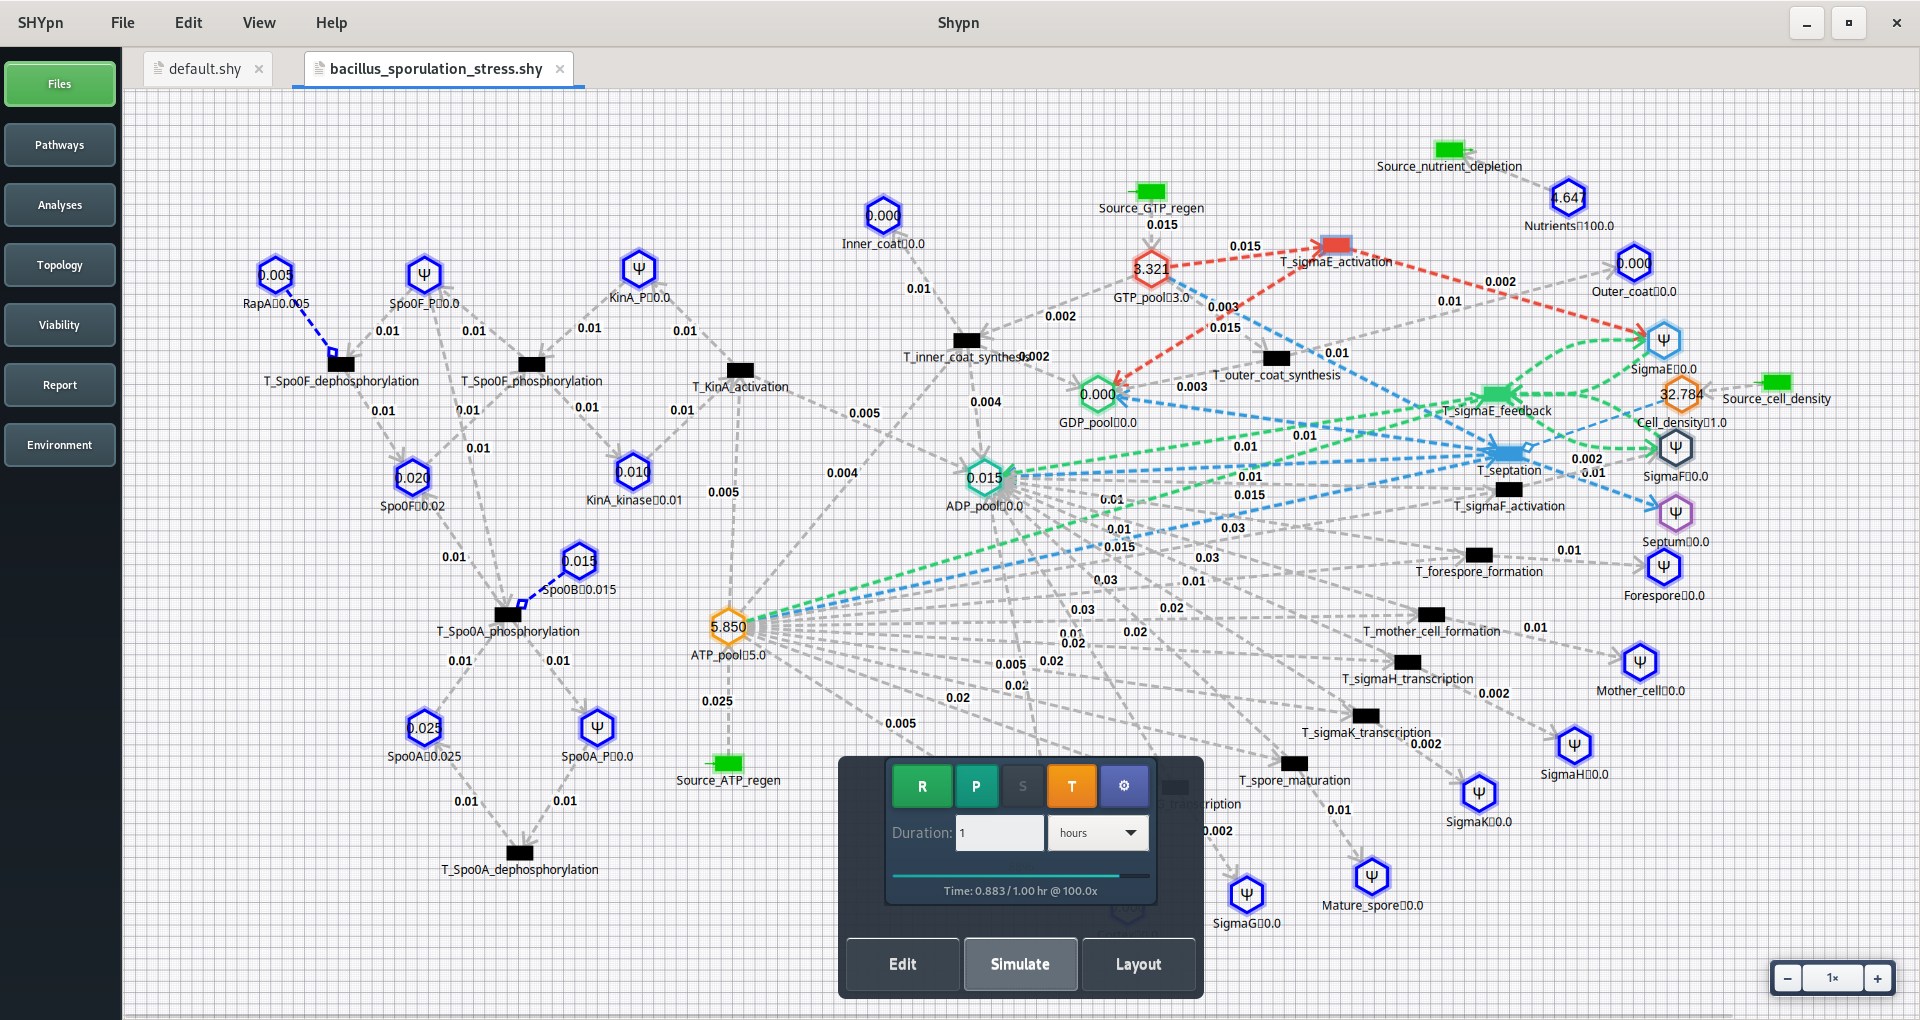
\includegraphics[width=\textwidth]{figures/Panels_SHYpn.png}
\caption{Fachada principal da SHYpn e paleta de painéis: cada painel
encapsula um contexto computacional persistente — construção de modelo,
simulação dinâmica, análise topológica, verificação de viabilidade e
geração de relatórios — permitindo navegação não linear entre fases
do fluxo de trabalho.}
\label{fig:panels-shypn}
\end{figure}

A SHYpn implementa uma \textbf{arquitetura multi-painel de documentos
persistentes} inspirada em ambientes de desenvolvimento integrado modernos
como Visual Studio Code, onde painéis especializados organizam a funcionalidade
por fase do fluxo de trabalho.

Cada painel funciona como um contexto computacional persistente com estado
independente.
O \textbf{Painel de Arquivos} (\textit{Explorer}) gerencia exclusivamente o
sistema de arquivos do projeto: árvore de diretórios, navegação
(avançar, retroceder, raiz), criação e abertura de projetos, e operações de
persistência (salvar, salvar como).
A \textbf{Tela de Modelagem} (\textit{Canvas}) é a superfície gráfica sobre
a qual o pesquisador constrói e edita o modelo: posiciona lugares e
transições, traça arcos, edita propriedades de cada objeto via diálogos
contextuais (marcação inicial, tipo de transição, constantes cinéticas,
designação de lugares de sinal $\Psi \subset P$) e instancia parâmetros
diretamente nos objetos do modelo.
O \textbf{Painel de Operações de Vias} (\textit{Pathway Operations})
constitui o centro de importação e enriquecimento paramétrico, reunindo
oito categorias: importação de vias KEGG (com conversão automática para
rede de Petri), importação de modelos SBML/BioModels, importação de modelos
genômicos BiGG, enriquecimento cinético via BRENDA (consulta por número EC
com seleção manual de parâmetros), enriquecimento via SABIO-RK (base pública
sem autenticação), inferência heurística de parâmetros baseada em tipo de
transição, histórico de enriquecimentos com rastreabilidade e avaliação, e
configuração termodinâmica universal.
A partir deste painel, modelos de fontes curadas são importados e traduzidos
diretamente para o formalismo SHPN; modelos que carecem de parâmetros cinéticos
podem ser inspecionados e enriquecidos consultando valores do BRENDA e SABIO-RK,
com edição interativa dos parâmetros selecionados.
A Figura~\ref{fig:e-coli-core} exemplifica a importação via Painel de
Operações de Vias: o modelo metabólico central de \textit{E.~coli}
(\textit{e\_coli\_core}) foi importado diretamente do repositório BiGG,
traduzido para rede de Petri e carregado na Tela de Modelagem para edição.

\begin{figure}[htbp]
\centering
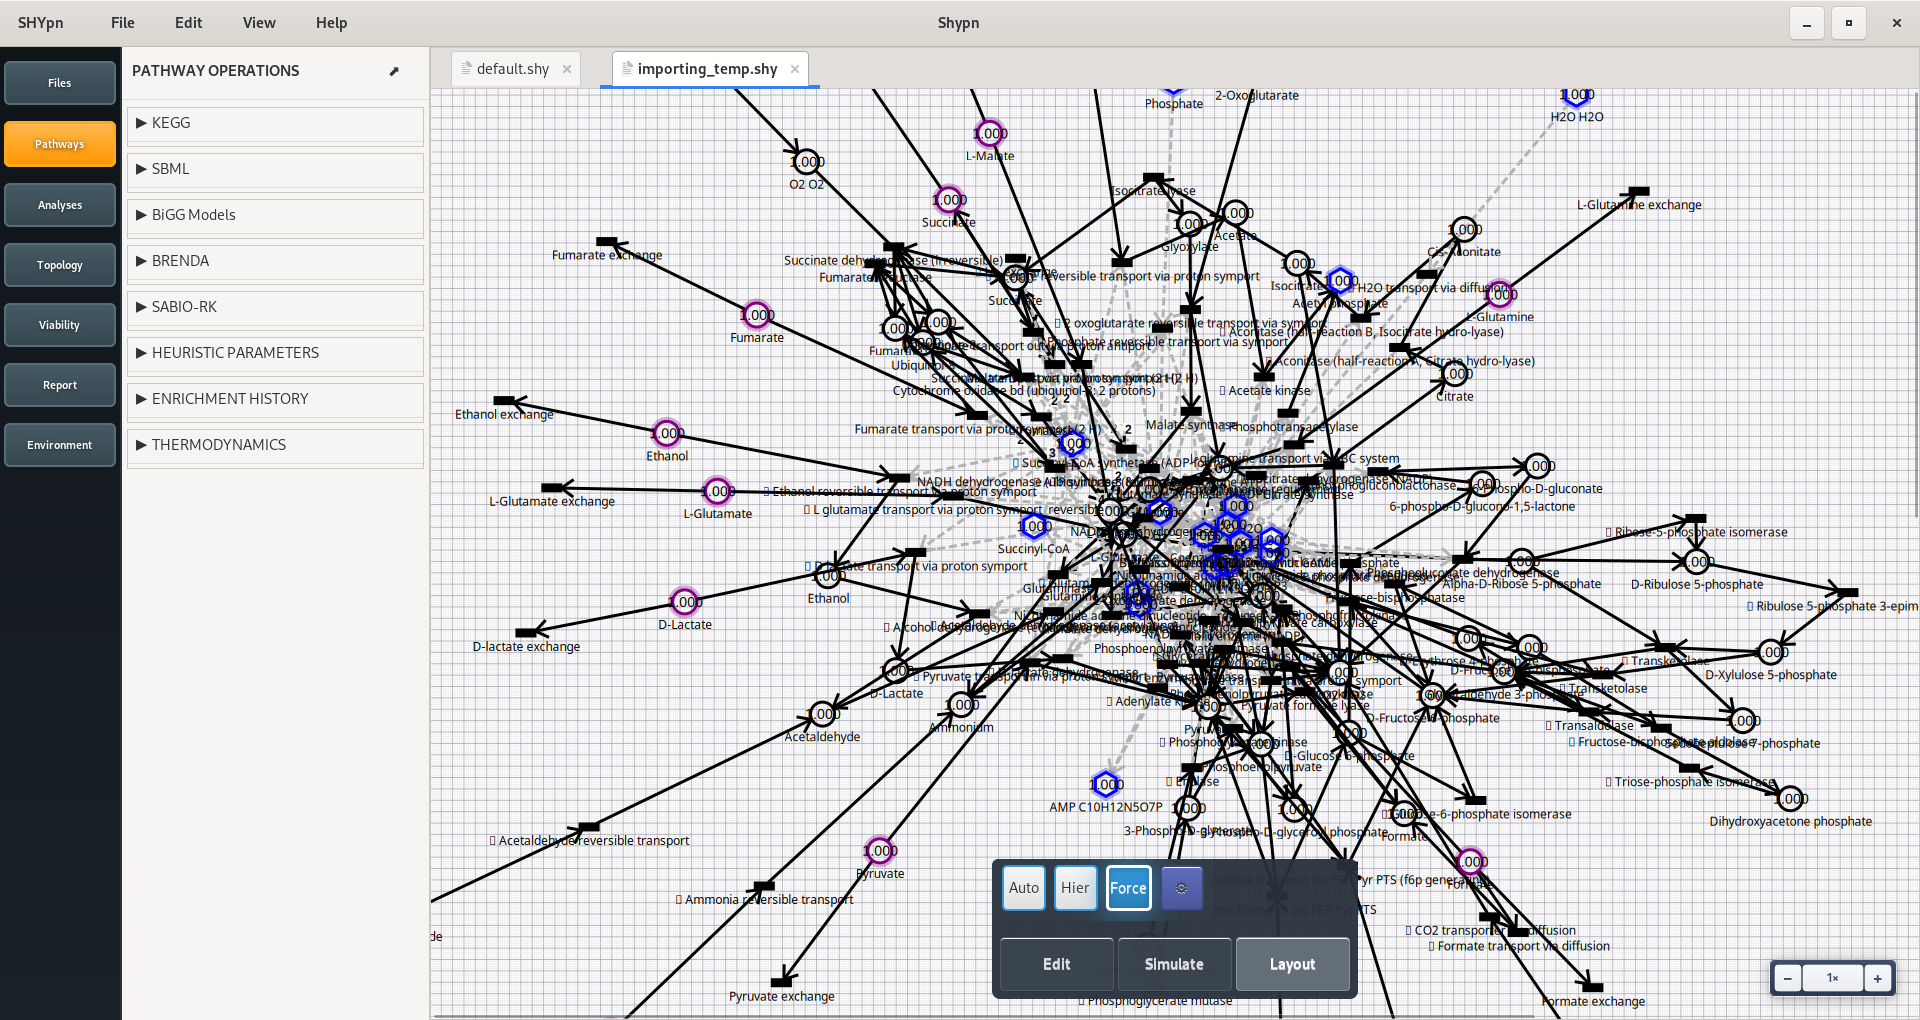
\includegraphics[width=\textwidth]{figures/e_coli_core.png}
\caption{Importação do modelo \textit{e\_coli\_core} a partir do
repositório BiGG via Painel de Operações de Vias: a SHYpn recupera
automaticamente a topologia SBML, converte para rede de Petri e
carrega o modelo na Tela de Modelagem para edição e simulação.}
\label{fig:e-coli-core}
\end{figure}

O \textbf{Painel de Análise} mantém o estado de simulação dinâmica com
atualização de gráficos de trajetória a 10~Hz, automação de varredura de
parâmetros e gerenciamento de réplicas estocásticas.
O \textbf{Painel de Topologia} calcula propriedades estruturais da rede —
P-invariantes representando leis de conservação, T-invariantes enumerando ciclos
de reação, análise do grafo regulatório revelando \textit{alças de retroalimentação},
\textit{hubs} e coeficientes de agrupamento, além de verificação de
vivacidade e limitação.
O \textbf{Painel de Viabilidade} isola a análise de sub-rede para investigação
focada: detecta componentes faltantes (substratos, catalisadores, produtos),
tenta verificar balanço elementar por consulta ChEBI ao nome dos compostos
--- quando a resolução é bem-sucedida --- e propõe correções estruturais
com capacidade de desfazer.
O \textbf{Painel de Relatório} sintetiza conteúdo de todos os painéis em
documentação pronta para publicação — tabelas de estrutura de modelo,
parâmetros, resultados de simulação, propriedades topológicas e registros de
correções de viabilidade, com exportação em PDF, Excel, JSON e Markdown.

\subsection{Sincronização entre Painéis}

Os painéis mantêm consistência por sincronização automática de dados.
Modificar a estrutura da rede na Tela de Modelagem desencadeia atualizações
imediatas: o Painel de Análise invalida resultados de simulação obsoletos, o
Painel de Topologia invalida P-invariantes em cache, o Painel de Viabilidade
atualiza a análise de dependências e o Painel de Relatório atualiza as
estatísticas de estrutura do modelo.
A sincronização respeita o custo computacional: atualizações leves (contagem de
lugares/transições) ocorrem imediatamente; recomputações custosas (P-invariantes,
análise de grafo regulatório) ocorrem sob demanda, sinalizadas por emblemas
visuais ``Desatualizado'' que solicitam atualização explícita.
Essa sincronização elimina uma fonte de erro comum na biologia computacional —
modelos modificados sem atualização da documentação correspondente.

\section{Painéis: Suporte ao Fluxo de Trabalho Biológico}
\label{sec:paineis}

\subsection{Painel de Arquivos: Gestão de Arquivos do Projeto}

A Figura~\ref{fig:explorer-panel} mostra o Painel de Arquivos aberto na
SHYpn, com a árvore de diretórios do projeto e os controles de navegação.

\begin{figure}[htbp]
\centering
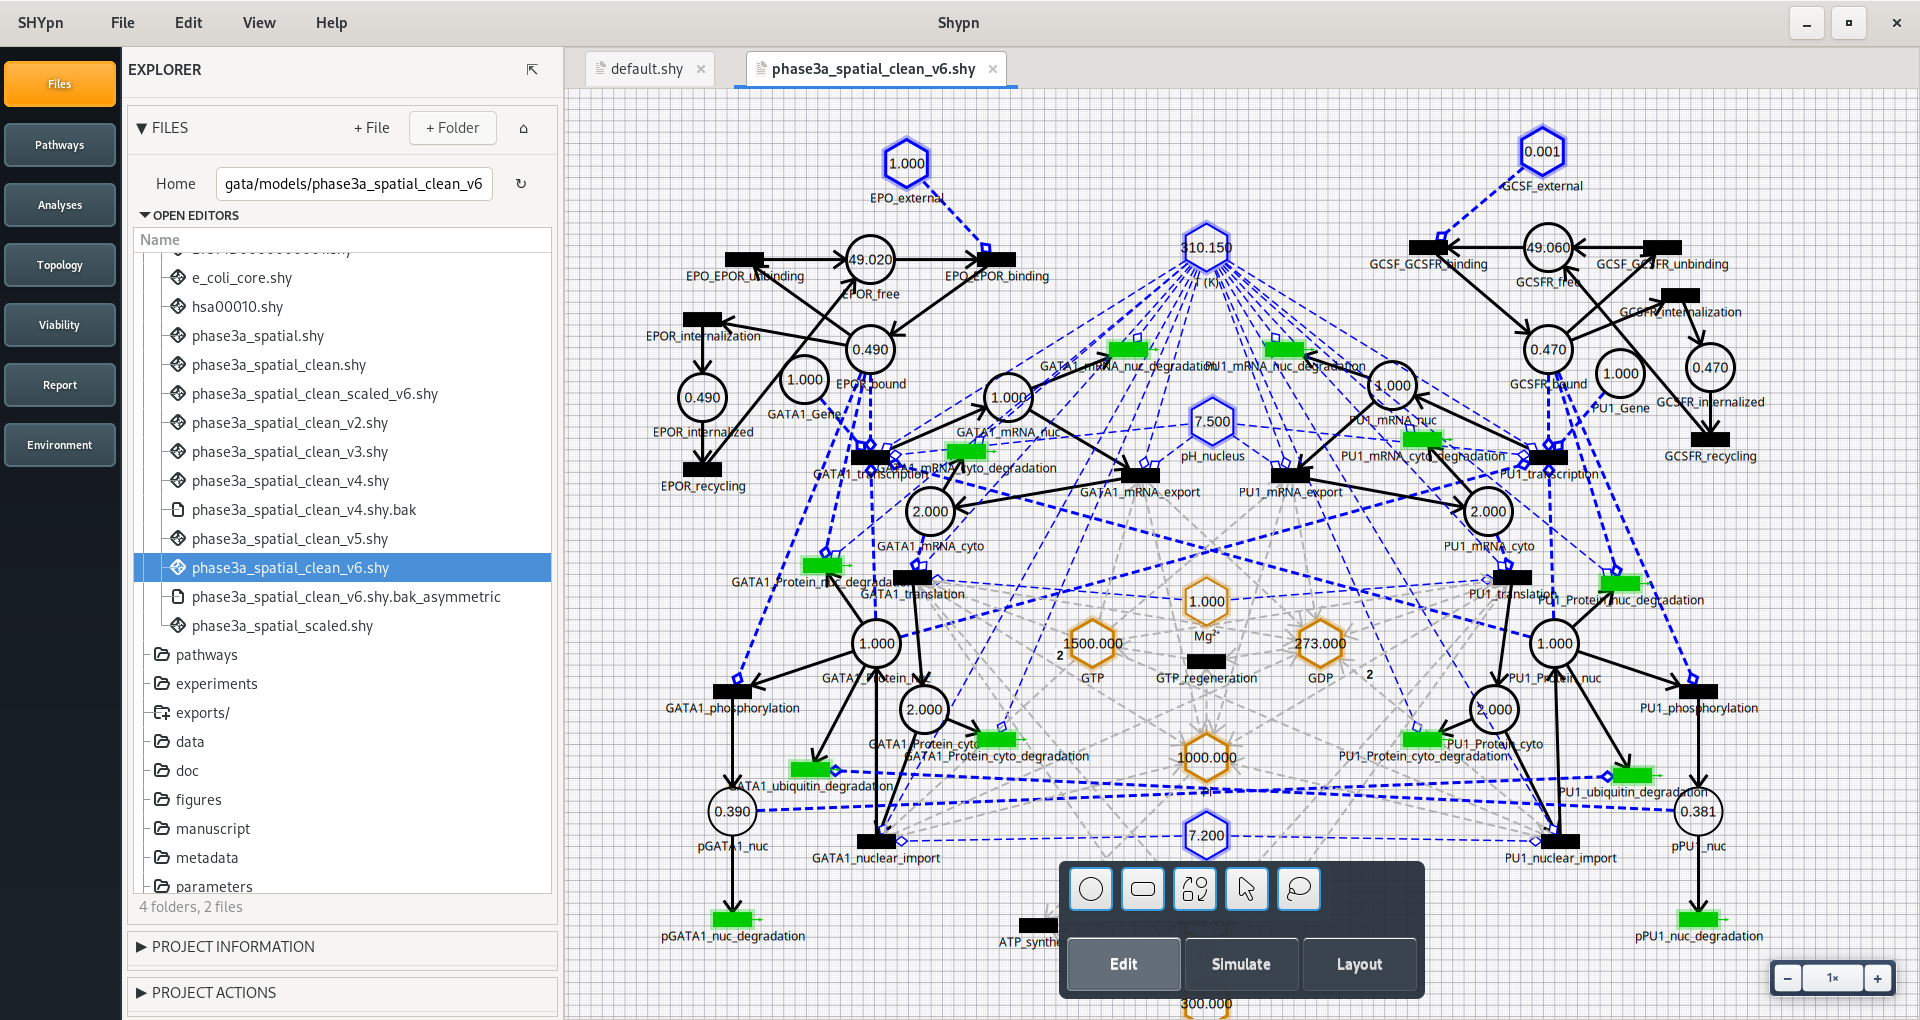
\includegraphics[width=\textwidth]{figures/explorer.png}
\caption{Painel de Arquivos (\textit{Explorer}) da SHYpn: árvore de
diretórios do projeto com navegação hierárquica, controles de
persistência (novo, abrir, salvar) e gestão de projetos.}
\label{fig:explorer-panel}
\end{figure}

O Painel de Arquivos (\textit{Explorer}) é exclusivamente dedicado à gestão
do sistema de arquivos do projeto.
Fornece uma árvore de diretórios com navegação completa (avançar, retroceder,
subir nível, voltar à raiz do projeto), barra de ferramentas para operações de
arquivo (novo, abrir, salvar, salvar como) e ações de projeto (novo projeto,
abrir projeto, configurações).
O Painel de Arquivos \emph{não} intervém na edição do modelo nem na atribuição
de parâmetros --- essas responsabilidades pertencem à Tela de Modelagem e ao
Painel de Operações de Vias, respectivamente.

\subsection{Tela de Modelagem: Desenho e Parametrização do Modelo}

A Tela de Modelagem (\textit{Canvas}) é a superfície gráfica central da SHYpn,
sobre a qual o pesquisador constrói visualmente a rede de Petri e instancia
parâmetros nos objetos do modelo.
A tela suporta documentos múltiplos com abas independentes, cada uma mantendo
um \texttt{ModelCanvasManager} com coleções isoladas de lugares, transições e
arcos, estado de zoom/pan e grade adaptativa.

A construção do modelo opera por interação direta: o pesquisador seleciona a
ferramenta adequada na paleta (\textit{SwissKnifePalette}) e clica na tela para
posicionar lugares e transições, ou arrasta entre objetos para traçar arcos.
Diálogos contextuais (acessados por duplo clique ou menu de contexto) permitem
editar cada propriedade: marcação inicial~$M_0(p)$, tipo de transição
(contínua, estocástica, temporizada, imediata), constantes cinéticas
($K_m$, $V_{\text{max}}$), peso de arcos e designação de lugares de sinal
($\Psi \subset P$).
A distinção visual emprega bordas azuis (lugares de sinal) \textit{versus} bordas
pretas (lugares normais), correspondendo ao modelo de validação do
\textit{Bacillus} (Capítulo~\ref{ch:validacao-bacillus}), onde os lugares de
sinal designados foram suficientes para produzir o limiar emergente de decisão.

A atribuição de parâmetros rastreia a proveniência por cor: valores padrão
importados do KEGG (células cinzas), medidas experimentais enriquecidas pelo
BRENDA (células azuis) e edições manuais do usuário (células laranja), permitindo
avaliar a confiança paramétrica --- modelos com 90\% de enriquecimento BRENDA
possuem embasamento empírico mais robusto.

\subsection{Painel de Operações de Vias: Importação e Enriquecimento}

O Painel de Operações de Vias (\textit{Pathway Operations}) constitui o centro
de importação de modelos e enriquecimento paramétrico da SHYpn, reunindo oito
categorias funcionais numa interface unificada.

\textbf{Importação de modelos curados.}
Três categorias permitem importar modelos diretamente de bases de dados curadas,
com conversão automática para o formalismo SHPN:
(i)~\textbf{KEGG} --- o usuário fornece um identificador de via (ex.: hsa00010)
e a SHYpn busca os dados KGML, analisa a via e converte-a em rede de Petri
com layout preservado;
(ii)~\textbf{SBML/BioModels} --- importação de arquivos SBML locais ou busca
remota no repositório BioModels, com detecção automática de compartimentos e
pós-processamento de layout;
(iii)~\textbf{BiGG} --- navegação e importação de modelos genômicos de escala
genômica a partir do repositório BiGG, com classificação automática de
lugares de sinal.

\paragraph{Mapeamento SBML $\to$ 13-tupla + grafo de parâmetros.}
A importação SBML não é mera tradução sintática: a SHYpn classifica os
elementos do documento SBML nas categorias semânticas do formalismo SHPN
(Capítulo~\ref{ch:shpn}, Tabela~\ref{tab:decisoes-modelador}). Cada
\texttt{species} torna-se um lugar $p \in P$, com a anotação
\texttt{compartment} preservada como metadado e usada pelo
\textit{compartment-module service} para induzir a partição em módulos.
Cada \texttt{reaction} torna-se uma transição $t \in T$ com tipo $\Phi(t)$
derivado da \textit{kinetic law} (contínua quando há lei explícita,
estocástica quando o anotador SBO sinaliza Hill ou Mass Action discreto).
Os \texttt{reactants} e \texttt{products} mapeiam para arcos $F$ com pesos
estequiométricos; os \texttt{modifiers} requerem desambiguação semântica:
ausentes da lei cinética ou anotados como catálise são convertidos em
arcos de teste $F_t$; presentes na lei com termo de Hill ou cooperatividade
notacionalmente compatível com $\Gamma$ são promovidos a arcos de fluxo de
sinal $F_s$ e o lugar correspondente é anexado a $\Psi$.

Os \texttt{parameters} globais e os \texttt{initial assignments} do SBML
não entram na rede-objeto: são instanciados como \textbf{lugares de
parâmetro} ($\Box$, \texttt{is\_parameter\_place=true}) no \emph{grafo de
parâmetros} separado, e os \texttt{events} do SBML preservam-se como
eventos do plano experimental (Capítulo~\ref{ch:shpn},
Seção~\ref{sec:planejamento-experimental}). Essa separação
rede-objeto / plano experimental --- ausente no documento SBML original
--- materializa-se durante a importação e é condição necessária para que o
modelo importado se beneficie das varreduras paramétricas e da
proveniência hierárquica descritas adiante.
Metadados curatoriais (anotações MIRIAM, referências cruzadas a ChEBI, KEGG,
UniProt, e o próprio identificador BioModels do documento de origem) são
retidos como propriedades por objeto, permitindo rastrear cada elemento
da rede SHPN até sua origem no SBML curado.

\textbf{Enriquecimento paramétrico.}
Modelos importados frequentemente carecem de constantes cinéticas.
Três categorias resolvem essa lacuna:
(i)~\textbf{BRENDA} --- após autenticação, o pesquisador consulta o BRENDA por
número EC ou nome de reação, visualiza os parâmetros cinéticos disponíveis
($K_m$, $k_{\text{cat}}$, $V_{\text{max}}$) e seleciona manualmente quais
aplicar ao modelo;
(ii)~\textbf{SABIO-RK} --- base de dados pública (sem autenticação) com o
mesmo fluxo de consulta e seleção manual;
(iii)~\textbf{Inferência Heurística} --- inferência inteligente de parâmetros
com base no tipo de transição (contínua, estocástica, temporizada, imediata)
e contexto biológico, aprendendo do histórico de enriquecimentos anteriores.

A categoria \textbf{Histórico de Enriquecimentos} permite rastrear, avaliar e
desfazer aplicações de parâmetros, garantindo rastreabilidade completa.
A categoria \textbf{Termodinâmica} configura as definições de validação
termodinâmica universal e mapeamento de compostos.

\subsection{Painel de Análise: Simulação Dinâmica}

O Painel de Análise expõe controle de simulação e visualização de trajetórias
em tempo real.
A Figura~\ref{fig:dynamic-analysis} ilustra a interface desse painel,
com os controles de simulação e a visualização de trajetórias dinâmicas.

\begin{figure}[htbp]
\centering
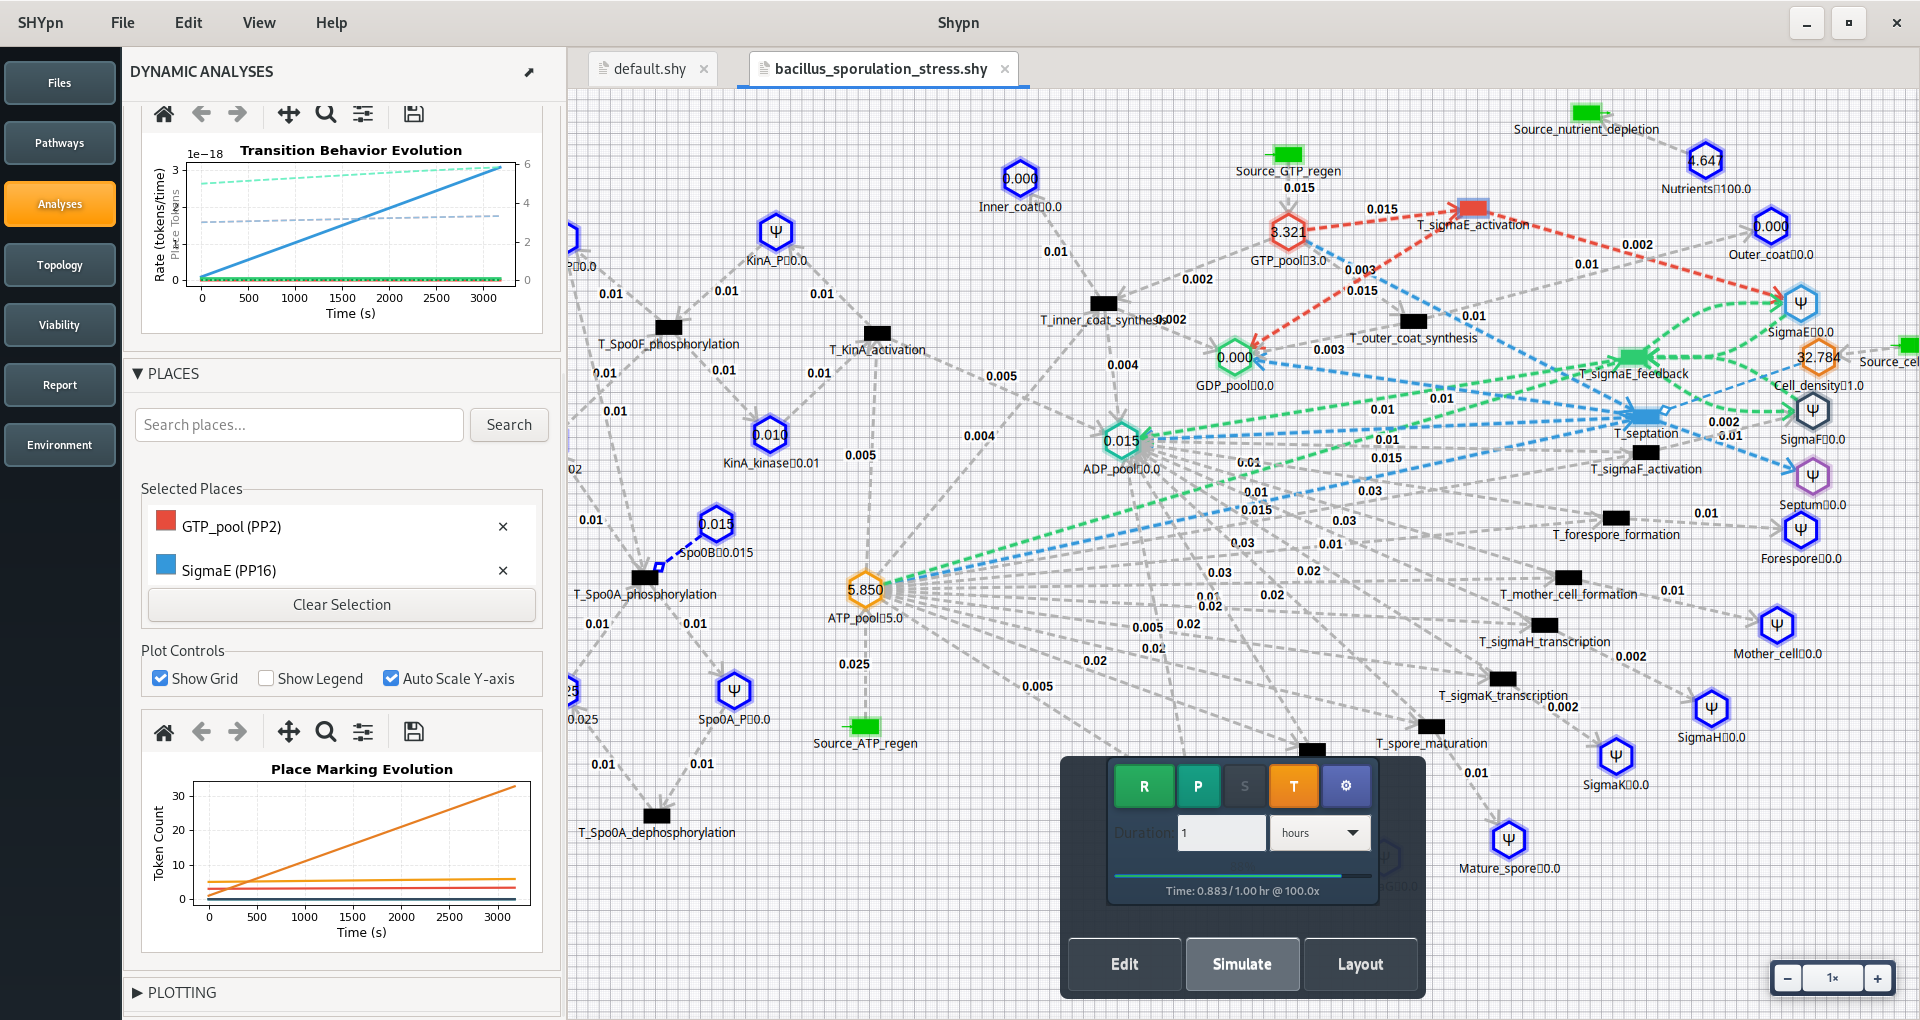
\includegraphics[width=\textwidth]{figures/Dynamic_analysis.png}
\caption{Painel de Análise Dinâmica da SHYpn: controles de simulação
(duração, passo, solver), gráficos de trajetória atualizados em tempo
real e sobreposições de limiar para identificação de regimes regulatórios.}
\label{fig:dynamic-analysis}
\end{figure}

Pesquisadores configuram parâmetros de simulação (duração, passo de tempo,
seleção de solver de EDO, contagem de réplicas estocásticas), iniciam a execução
e observam a evolução de marcação $M(p, t)$ por gráficos atualizados
dinamicamente.
Sobreposições de limiar marcam concentrações biologicamente significativas
($[\sigma^H] = \theta_{\sigma H} \approx 1{,}60\,\mu$M, $[\text{Spo0A}{\sim}\text{P}] = 20\ \mu$M),
alertando quando simulações entram em regimes regulatórios preditos.
A automação de varredura de parâmetros explora espaços multidimensionais:
variando $K_m$ de 0,01 a 1~mM (10 etapas logarítmicas) com $V_{\text{max}}$
de 1 a 10~mM/s (10 etapas lineares) gera uma grade 10$\times$10 de simulações,
com visualização em mapa de calor revelando relações compensatórias.
O modo de simulação estocástica executa 100 ou mais réplicas com sementes
aleatórias independentes, quantificando o ruído intrínseco: o coeficiente de
variação CV~=~$\sigma/\mu$ revelou variabilidade celular de $\sim\!15\%$ na
ativação do fator sigma durante a validação da esporulação do
\textit{Bacillus}, compatível com distribuições experimentais.

\subsection{Painel de Topologia: Análise Estrutural}

A Figura~\ref{fig:topology-panel} mostra o Painel de Topologia durante a
execução de análises estruturais e comportamentais do modelo GATA, com os
resultados de P-invariantes, T-invariantes e propriedades do grafo regulatório.

\begin{figure}[htbp]
\centering
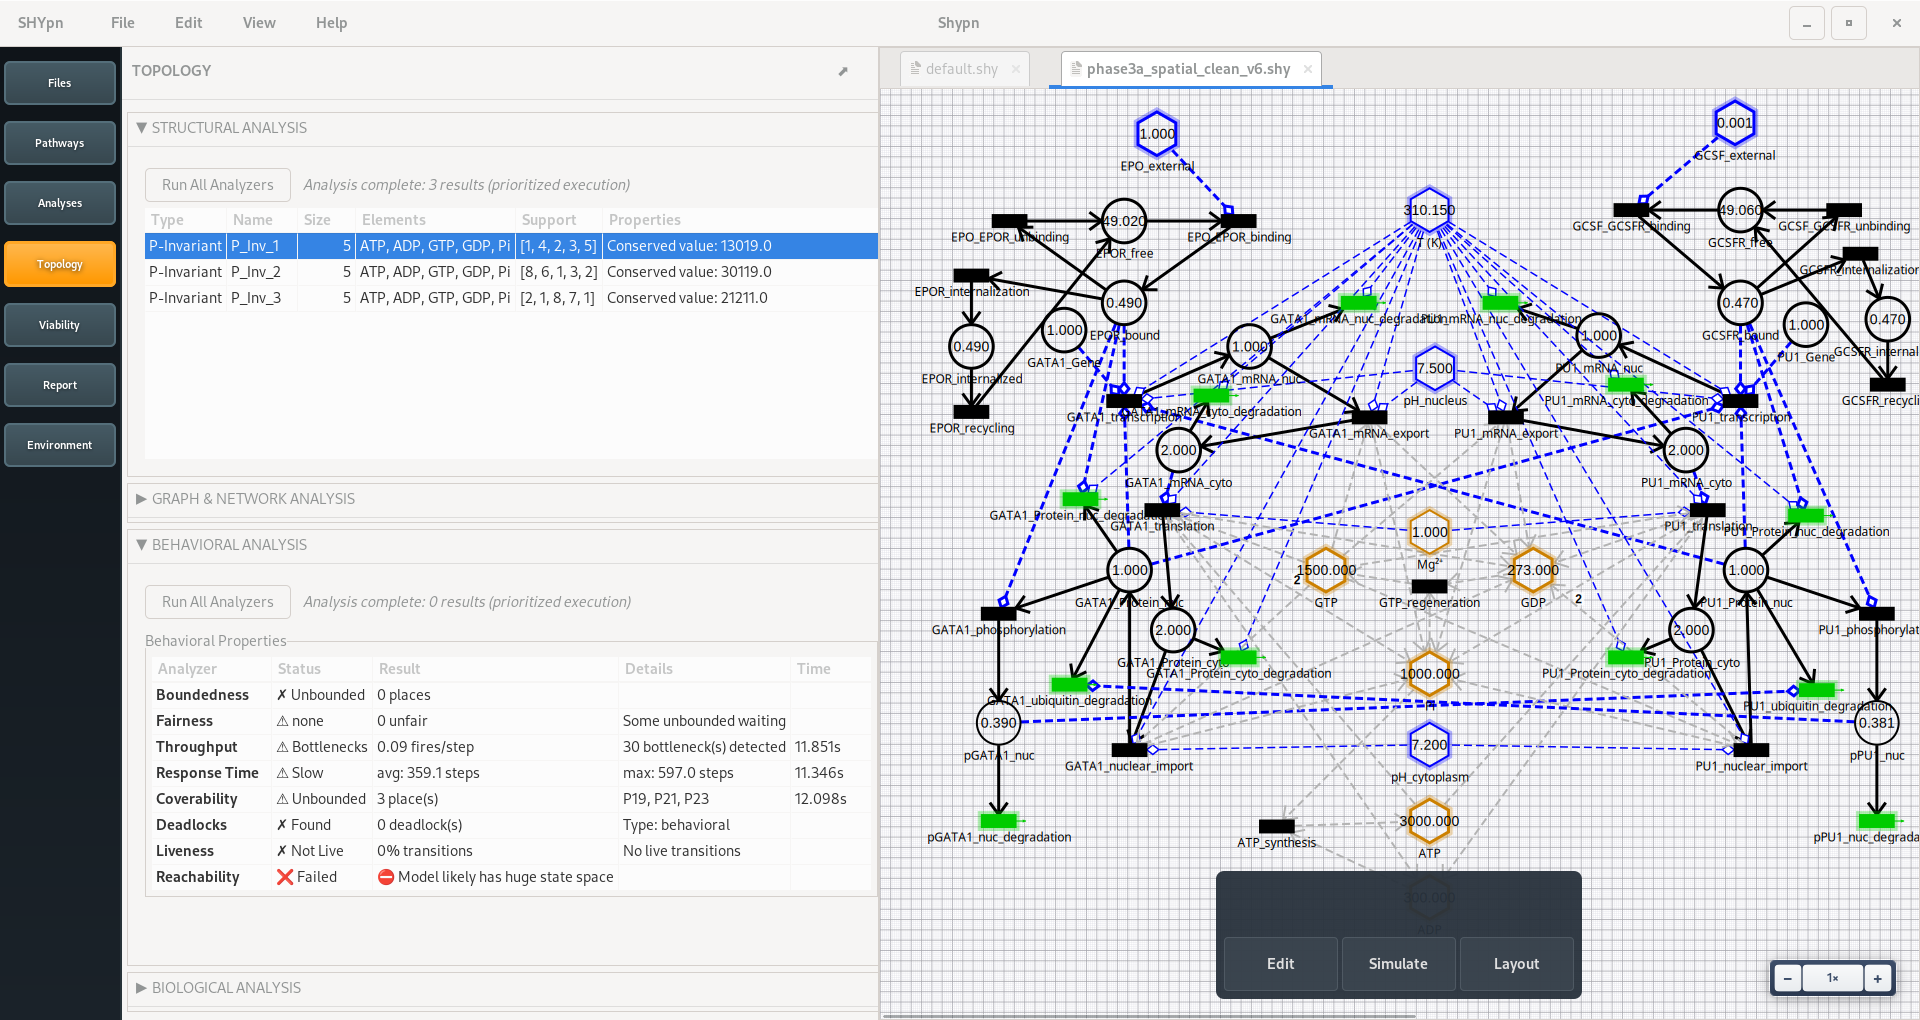
\includegraphics[width=\textwidth]{figures/Topology.png}
\caption{Painel de Topologia da SHYpn executando análise estrutural e
comportamental do modelo GATA: a interface exibe P-invariantes (leis de
conservação), T-invariantes (ciclos de reação) e propriedades do grafo
regulatório, permitindo validação da conectividade da rede antes da
simulação dinâmica.}
\label{fig:topology-panel}
\end{figure}

O Painel de Topologia calcula propriedades de rede independentes de parâmetros
cinéticos, revelando capacidades e restrições inerentes à conectividade da rede.
A \textbf{análise estrutural} identifica P-invariantes (leis de conservação como
ATP~+~ADP~+~AMP~=~const) e T-invariantes (ciclos de reação como o ciclo de
glicose~6-fosfato).
A \textbf{análise de grafos} constrói grafos regulatórios a partir de arcos de
teste e de inibição, detectando \textit{alças} de retroalimentação positivas
(que impulsionam biestabilidade) e negativos (que permitem oscilações), além
de classificar hubs como ATP, NAD$^+$ e CoA.
A \textbf{análise de dependências} aplica a classificação de independência fraca
do Capítulo~\ref{ch:shpn} para particionar pares de transições em
independentes (lugares de entrada disjuntos), fracamente dependentes
(entradas somente leitura compartilhadas) e fortemente acoplados (operações de
escrita conflitantes), habilitando simulação paralela com \textit{speedup}
de 1,9$\times$ para o modelo do \textit{Bacillus} em 4 núcleos.
As leis de conservação são verificadas numericamente
após cada passo da simulação, com tolerância $\| C^T \cdot M(t) \| < 10^{-6}$.

\subsection{Painel de Viabilidade: Refinamento Inteligente}

A Figura~\ref{fig:viability-panel} mostra o Painel de Viabilidade durante
uma varredura por planejamento fatorial, onde combinações de parâmetros são
exploradas sistematicamente para avaliar a robustez do modelo.

\begin{figure}[htbp]
\centering
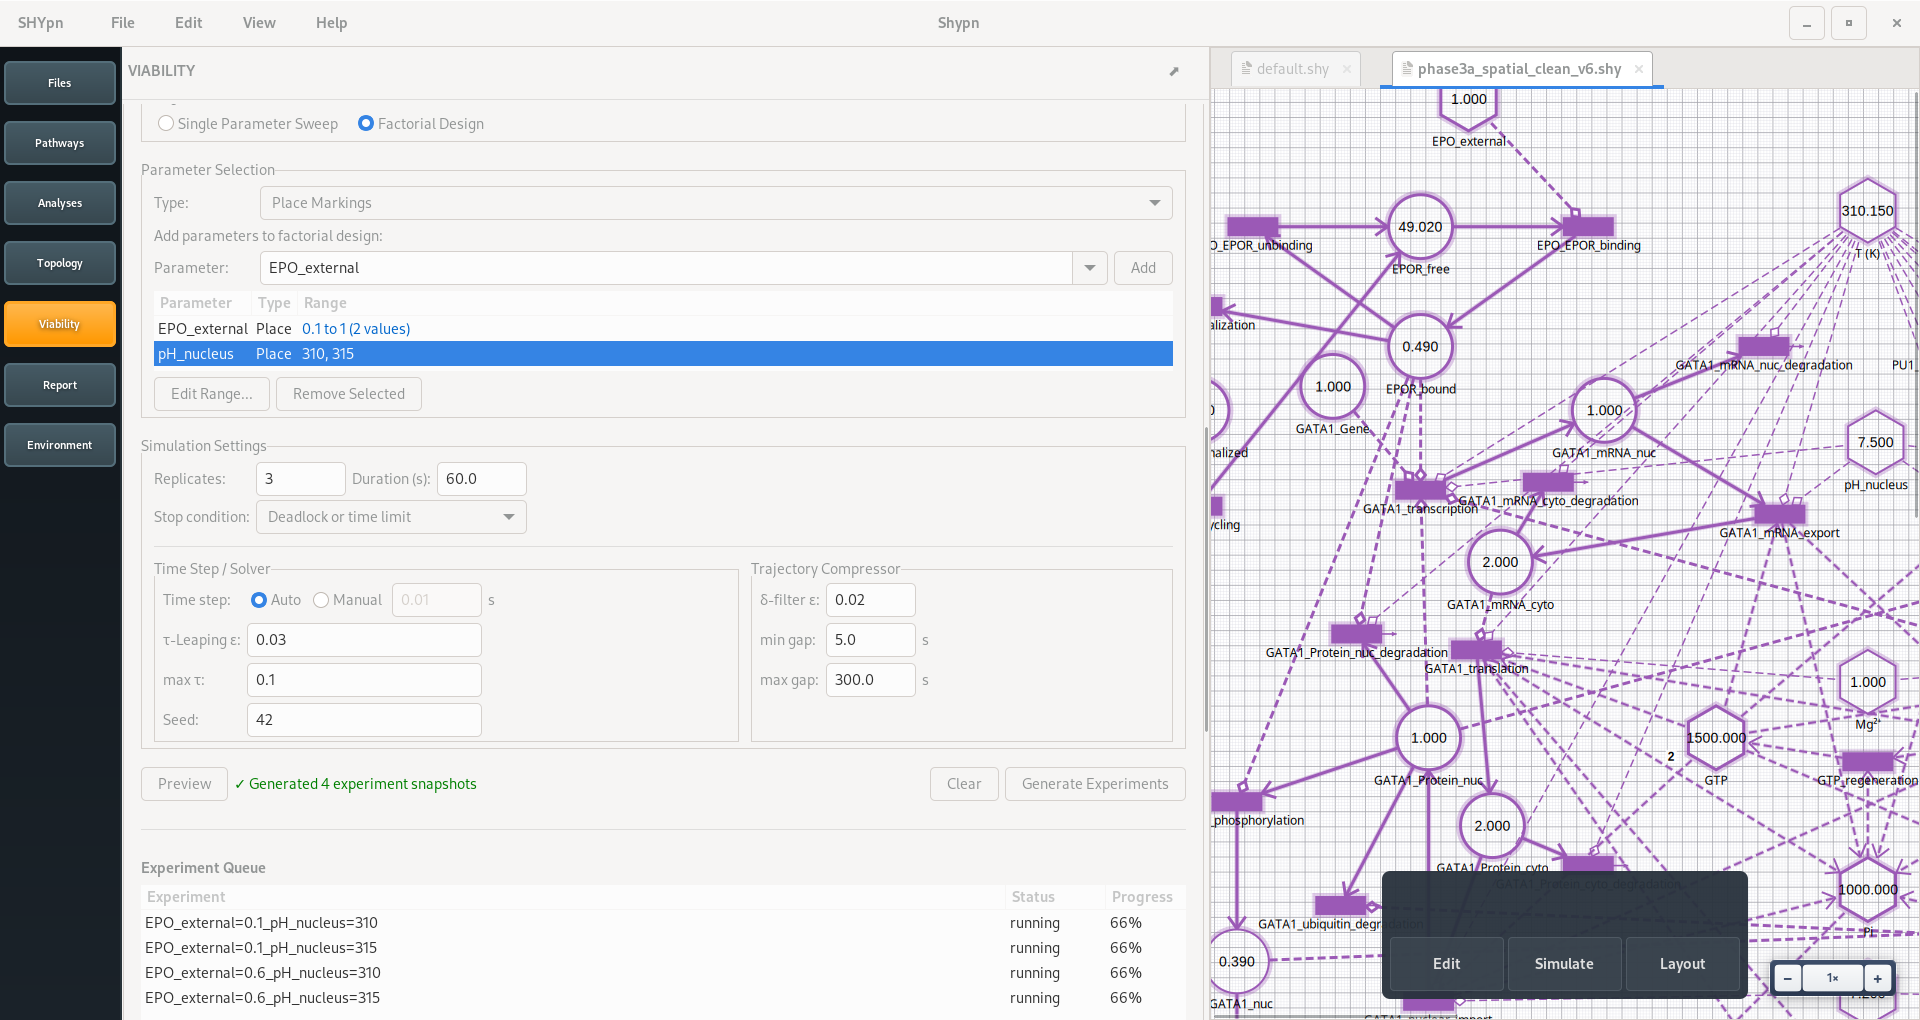
\includegraphics[width=\textwidth]{figures/Viablity.png}
\caption{Painel de Viabilidade da SHYpn executando uma varredura por
planejamento fatorial: os analisadores especializados verificam
dependências, disponibilidade de substratos e balanço elementar,
enquanto a varredura paramétrica identifica regiões de operação viável
do modelo.}
\label{fig:viability-panel}
\end{figure}

Modelos biológicos crescem incrementalmente; o rastreamento manual de
dependências falha para redes com mais de cerca de 20 componentes.
O Painel de Viabilidade automatiza a detecção de dependências por quatro
analisadores especializados.
O \textbf{Analisador de Localidade} verifica a disponibilidade de substratos,
presença de catalisadores e consumo de produtos.
O \textbf{Analisador de Dependências} consulta bases de conhecimento
bioquímico — quinases requerem ATP, transcrição necessita nucleotídeos,
fosforilação libera ADP — para detectar lógica regulatória ausente.
O \textbf{Analisador de Fronteira} examina lugares de oferta infinita
conferindo plausibilidade termodinâmica.
O \textbf{Analisador de Conservação} tenta verificar o balanço elementar
consultando o ChEBI pelo nome de cada composto; nos casos em que a
resolução é unívoca, o módulo exige conservação de C, H, O, N e P.
A heterogeneidade de notações de nomes limita a cobertura, e não há
interface para entrada manual de fórmulas.
O fluxo de 22 transições do modelo do \textit{Bacillus} exigiu dezenas de
iterações de refinamento; o Painel de Viabilidade identificou
arcos de teste faltantes ao longo desse processo.

\section{Arquitetura Dual do Motor de Simulação}
\label{sec:motores-simulacao}

O Capítulo~\ref{ch:shpn} define a evolução da marcação por regra
de disparo: $M(t+\Delta t) = M(t) + C \cdot \vec{v}(t)$, onde~$C$ é a matriz
estequiométrica e $\vec{v}(t)$ o vetor de taxas de disparo.
Essa abstração oculta complexidade de implementação significativa; a SHYpn a
aborda com uma \textbf{arquitetura dual} que suporta dinâmicas contínua (baseada
em EDO) e estocástica (Gillespie) com escalonamento hierárquico unificado.

\subsection{Motor Contínuo: Integração de EDO}

Reações metabólicas operando em grandes populações moleculares exibem
dinâmicas determinísticas bem aproximadas por EDOs.
O motor contínuo executa cinco etapas coordenadas.

\textbf{Avaliação da função de taxa:} para cada transição $t \in T$, avalia-se
$r(t, M)$ com as leis cinéticas suportadas: ação de massa ($r = k \cdot \prod M(p)$),
Michaelis-Menten ($r = V_{\text{max}} \cdot M(S) / (K_m + M(S))$), Hill
($r = V_{\text{max}} \cdot M(S)^n / (K_d^n + M(S)^n)$) e expressões Python
personalizadas.

\textbf{Gateamento por limiar via $\Gamma$:} para cada lugar de sinal
$p_s \in \Psi$ com parâmetro termodinâmico associado, computa-se o limiar
efetivo $\theta_{\text{eff}}(p_s) = K \cdot (\varepsilon /
(1 - \varepsilon))^{1/n}$ e a função indicadora
$\Theta(p_s, M) = \mathbf{1}[M(p_s) \geq \theta_{\text{eff}}(p_s)]$.
Multiplica-se a taxa de transição pelo produto dessas funções indicadoras:
$v(t) = r(t, M) \cdot \prod_{(p_s,t) \in F_s} \Theta(p_s, M)$,
implementando o predicado de habilitação da
Definição~\ref{def:habilitacao} do Capítulo~\ref{ch:shpn}.

\textbf{Preempção hierárquica:} transições são particionadas por camada, computa-se
a camada mínima ativa $\lambda_{\min}$, e todas as transições com
$\lambda(t) > \lambda_{\min}$ são desabilitadas com $v(t) = 0$, implementando
a preempção de camada (Teorema~\ref{thm:preempcao}).

\textbf{Integração do sistema de EDO:} monta-se $dM/dt = C \cdot \vec{v}(M, t)$
e integra-se com Runge--Kutta de 4ª ordem (RK4) de passo fixo, acoplado
à amostragem $\tau$-leaping (Subseção~\ref{subsec:motor-estocastico})
por divisão de operador (\emph{operator splitting}) por passo de tempo:
fluxo contínuo $\to$ disparos estocásticos $\to$ finalização.

\textbf{Verificação de leis de conservação:} após cada passo de tempo,
verifica-se $\|C^T \cdot M(t)\| < 10^{-6}$; violações acionam avisos que
indicam erros estequiométricos ou instabilidade numérica.
Este motor simula o modelo do \textit{Bacillus} (40~lugares e
36~transições --- ver
Capítulo~\ref{ch:validacao-bacillus}) em tempo de parede inferior a 5~s
(21.600~s de tempo biológico).

\subsection{Motor Estocástico: $\tau$-leaping}
\label{subsec:motor-estocastico}

Espécies regulatórias com baixo número de cópias ($\sim\!100$ moléculas de
fatores de transcrição, $\sim\!10$ moléculas de mRNA) exibem flutuações
estocásticas onde a aproximação determinística por EDO falha.
O motor estocástico implementa o algoritmo \textbf{$\tau$-leaping}
(\textcite{Gillespie2001}), uma aproximação acelerada do SSA exato de
\textcite{Gillespie1977} --- cuja variante eficiente por grafo de dependências
é o método de \textcite{Gibson2000} --- adaptada para redes de Petri hierárquicas: em
cada passo $\tau$, o número de disparos de cada transição é amostrado de
uma distribuição de Poisson com média $a(t,M)\cdot\tau$, em vez de
selecionar uma única reação por evento como no SSA exato.
Reações reversíveis acopladas (forma $A \rightleftharpoons B$ detectadas
por convenção de nomenclatura $k_f / k_r$) são amostradas pelo estimador
Skellam (Poisson direta menos Poisson reversa) para correto tratamento
do balanço detalhado.

Para cada transição $t$, a propensão é
\[
  a(t, M) = r(t, M) \cdot \prod_{p \in \bullet t} \binom{M(p)}{W((p,t))},
\]
levando em conta combinações moleculares discretas.
O gateamento por limiar e a preempção hierárquica são aplicados de forma
idêntica ao motor contínuo, zerando $a(t)$ para transições desabilitadas.
A cada passo, o tamanho $\tau$ é selecionado adaptativamente de modo a
limitar a variação relativa esperada de cada espécie a uma fração
configurável (controle de erro $\varepsilon_\tau$); para cada transição,
amostra-se o número de disparos $k_t \sim \mathrm{Poisson}(a(t,M)\cdot\tau)$
e a marcação é atualizada por $M' = M + \sum_t k_t \cdot C_t$, onde $C_t$ é
a coluna estequiométrica de $t$.
O modo híbrido trata modelos que misturam metabolismo contínuo (ATP e glicose
de alta cópia) com regulação discreta (fatores sigma de baixa cópia),
particionando automaticamente as transições em subconjuntos integrados por EDO
e amostrados por $\tau$-leaping com base nas marcações dos lugares, acoplando
os subsistemas por lugares compartilhados.
Um tipo \emph{adaptativo} adicional --- detalhe de implementação, não
primitivo do formalismo --- alterna automaticamente entre os modos contínuo
e estocástico por transição, com base no volume de compartimento e em um
limiar de número de cópias configurável.
A simulação estocástica do modelo do \textit{Bacillus} completou-se em 4,1~s
(réplica única); varreduras de parâmetros de 100 simulações em modo paralelo
(4 núcleos) finalizaram em 1,2~min (3,2$\times$ de \textit{speedup}).

\section{Qualidade de Implementação}
\label{sec:qualidade-implementacao}

\subsection{Pilha de Tecnologias}

A SHYpn utiliza Python~3.10+ para flexibilidade de domínio biológico com
desempenho por vetorização NumPy nos laços de avaliação de função de taxa
e, opcionalmente, por aceleração GPU via CuPy (\texttt{GPUHybridEngine},
backend CUDA~12.x para placas com suporte a precisão dupla);
GTK3 para arquitetura multi-janela com integração nativa de sistema
operacional e Matplotlib para gráficos de trajetória com qualidade de
publicação.
A integração com banco de dados emprega clientes de API REST consultando KEGG,
BRENDA e ChEBI com cache SQLite local que reduz requisições de rede e habilita
operação offline.
A persistência em JSON possibilita controle de versão Git, e contêineres Docker
que encapsulam o ambiente computacional completo garantem reprodutibilidade
bit-a-bit independentemente do sistema operacional do usuário.

\subsection{Métricas de Desempenho}

O modelo do \textit{Bacillus} (40~lugares e 36~transições) simula 6~h de
tempo biológico em tempo de parede inferior a 5~s no motor de EDO.
O Painel de Análise atualiza gráficos a 10~Hz durante a simulação sem atraso
perceptível, com buffers de trajetória armazenando 10.000 pontos temporais
($\sim\!12$~MB por modelo) e habilitando zoom e panorâmica dinâmicos.
O cálculo de P-invariantes (decomposição SVD de $C^T$) completa-se em menos de
1~s para o modelo do \textit{Bacillus} (matriz $40 \times 36$) e em 8,3~s para
redes de escala genômica (200 lugares $\times$ 150 transições).
O Painel de Viabilidade executa simulações de sub-rede (15 transições, 10 lugares)
em 0,3~s, habilitando ciclos interativos de refinamento de $\sim\!5$~s.
A pegada de memória do modelo do \textit{Bacillus} permanece dentro das
restrições de laptop, com escalonamento linear para redes de escala genômica.

\subsection{Garantia de Qualidade}

A cobertura de testes é de 87\% para os motores de simulação e de 68\% para
os componentes de interface, com 427 testes unitários verificando comportamento
individual de componentes: testes do motor de EDO comparam trajetórias simuladas
com soluções analíticas (decaimento exponencial, crescimento logístico), e
testes do motor de Gillespie verificam cálculos de propensão e distribuições de
amostragem de eventos.
Vinte e dois testes de integração executam fluxos completos — importação KEGG,
enriquecimento BRENDA, simulação, exportação de relatório — em exemplos de
validação (Capítulo~\ref{ch:validacao-bacillus}).
Asserções em tempo de execução verificam a preservação de P-invariantes após
cada passo de simulação mediante $\|C^T \cdot M(t)\| < 10^{-6}$; violações
interrompem a execução com diagnóstico detalhado.

\section{Síntese do Capítulo}
\label{sec:sintese-implementacao}

A plataforma SHYpn traduz o formalismo SHPN em maquinaria de simulação
executável por meio de três princípios: arquitetura multi-painel com
sincronização automática (Seção~\ref{sec:arquitetura-multi-painel}),
duplo motor de simulação EDO/Gillespie com escalonamento hierárquico
(Seção~\ref{sec:motores-simulacao}) e importação automatizada de modelos
com enriquecimento paramétrico (Seção~\ref{sec:paineis}).
A publicação em código aberto garante reprodutibilidade computacional.


\part{Síntese}
% cap_06_discussao.tex  –  Capítulo 6
% Discussão: SHPN como Formalismo Unificador
\chapter{Discussão: SHPN como Formalismo Unificador}
\label{ch:discussao}

Este capítulo discute as Redes de Petri Hierárquicas de Sinais como extensão
da teoria de Redes de Petri para modelagem de sistemas biológicos onde vias
metabólicas e redes regulatórias devem ser expressas sob um único formalismo.
A contribuição teórica evoluiu para uma \textbf{plataforma computacional de
experimentação \textit{in silico}}, habilitando investigação quantitativa em
biologia de sistemas, farmacocinética, biologia sintética e descoberta de
fármacos.
A discussão examina como essa unificação teórica habilita a predição
quantitativa de limiares de decisão, contextualiza o formalismo dentro
da teoria existente de Redes de Petri, explora quais questões de pesquisa a
plataforma computacional torna tratáveis e identifica problemas teóricos
abertos.

\section{Contribuição Teórica Central}
\label{sec:contribuicao-central}

As Redes de Petri Hierárquicas de Sinais estendem a teoria clássica de Redes
de Petri introduzindo três construtos formais que habilitam modelagem unificada
de vias metabólicas e redes regulatórias: a designação de lugares de sinal
($\Psi \subset P$), os arcos de fluxo de sinal
($F_s \subseteq (\Psi \times T) \cup (T \times \Psi)$)
e as funções de camada hierárquica ($\lambda: \Psi \to \mathbb{N}$).
Esses construtos resolvem uma limitação fundamental nos formalismos existentes
— a incapacidade de modelar controle regulatório por consumo molecular
simultaneamente à transferência de massa metabólica.

\subsection{Unificando Metabolismo e Regulação}

Redes de Petri biológicas clássicas representam vias metabólicas por lugares
(espécies moleculares) e transições (reações) conectados por arcos normais com
pesos estequiométricos.
Arcos de teste estendem esse modelo para catálise por leituras não consumidoras.
Contudo, redes regulatórias operam com semântica diferente: fatores de
transcrição habilitam a expressão gênica enquanto são consumidos em complexos
regulatórios; o ATP fornece energia para biossíntese enquanto a acumulação de Spo0A${\sim}$P
controla programas de desenvolvimento~\cite{Fujita2005}; e moléculas de
sinalização propagam informação por limiares de concentração enquanto são
degradadas ou sequestradas.

O desafio reside em que a mesma molécula participa de ambas as semânticas
simultaneamente — a dualidade metabólito-sinal motivada no
Capítulo~\ref{ch:introducao}.
Abordagens anteriores tratavam esses papéis separadamente, exigindo dois
paradigmas de modelagem distintos.
As SHPN unificam ambos por meio da partição de lugares $\Psi \subset P$: um
mesmo lugar $p \in \Psi$ pode ter arcos normais de entrada representando
produção metabólica e arcos de fluxo de sinal representando consumo regulatório,
formalizando matematicamente a participação dual.

Essa unificação torna três questões de pesquisa anteriormente intratáveis
formalmente expressas.
Em primeiro lugar, a \textbf{predição de limiar a partir de primeiros
princípios}: quando um estado de transição metabólica desencadeia uma
decisão regulatória irreversível?
Formalismos clássicos tratam limiares como parâmetros ajustados; a hierarquia
de sinais os deriva por análise de alcançabilidade, transformando a
identificação de limiar de ajuste de parâmetro em computação formal.
Em segundo lugar, a \textbf{análise composicional de acoplamento
metabólico-regulatório}: vias que compartilham intermediários metabólicos mas
possuem sinais regulatórios distintos ($\Psi_i \cap \Psi_j = \emptyset$) exibem
semântica composicional que habilita modelagem de escala genômica por
decomposição em módulos regulatórios independentes.
Em terceiro lugar, a \textbf{verificação de arquitetura de controle}: a preempção
de camada (Teorema~\ref{thm:preempcao}) impõe controle assimétrico —
sinais de camadas superiores controlam transições de camadas inferiores, mas
camadas inferiores não podem habilitar camadas superiores — tornando a
precedência biológica formalmente verificável.

\section{Posicionamento no Panorama da Teoria de Redes de Petri}
\label{sec:posicionamento-teoria}

A análise de lacunas do Capítulo~\ref{ch:fundamentos} identificou seis
limitações das extensões clássicas de Redes de Petri para modelagem biológica
multi-escala.
As SHPN estendem as Redes Híbridas com três construtos que endereçam essas
lacunas, preservando compatibilidade retroativa ($\Psi = \emptyset$ recupera a
semântica clássica).

A distinção teórica central é a \textbf{estratificação de semântica de arco}
em três categorias --- arcos normais (estequiometria), arcos de fluxo de sinal
(consumo regulatório unidirecional) e arcos de teste (catálise não consumidora)
--- que resolve uma limitação de expressividade: redes clássicas não distinguem
catálise, participação metabólica e controle regulatório.

A função de camada $\lambda$ introduz \textbf{arquitetura de controle formal}
com fluxo assimétrico e preempção hierárquica
(Teorema~\ref{thm:preempcao}), formalizando o princípio de que processos
essenciais (metabolismo) preemptam processos opcionais (diferenciação).
Nenhuma extensão clássica fornece semântica de precedência de controle
comparável~\cite{Simao2025HierarchicalPreemption}, e a verificação de conformidade reduz-se a travessia de grafo
em tempo polinomial.

A semântica de consumo transforma a predição de limiar: em lugar de codificar
limiares como parâmetros de Hill ajustados, o formalismo deriva
$\theta_{\text{eff}}$ analiticamente a partir de $\Gamma$ e identifica o ponto
de comprometimento sistêmico por análise de alcançabilidade
(Capítulo~\ref{ch:validacao-bacillus}).
A \textbf{teoria de independência fraca}
(Teorema~\ref{thm:independencia-fraca}) habilita decomposição composicional,
reduzindo a complexidade de $\mathcal{O}(\bar{M}^n)$ para
$\mathcal{O}(k \cdot \bar{M}^{n/k})$~\cite{Simao2025WeakIndependence,Simao2026QuorumSensing}.

Em síntese, as SHPN quebram três premissas que permeiam todos os formalismos
clássicos de Redes de Petri:

\begin{center}\small
\begin{tabular}{@{}p{3.8cm}p{3.8cm}p{4.5cm}@{}}
\toprule
Premissa clássica & SHPN & Consequência \\
\midrule
Habilitação é plana (verificação local apenas) &
  Habilitação é estratificada ($G_E \wedge$ Preempção) &
  Controle hierárquico representável sem conflação de massa e informação \\
\addlinespace
Todos os arcos são equivalentes (peso é peso) &
  Arcos $F_s$ carregam $\Gamma=(K,n,\varepsilon)$ &
  Limiar molecular, calibrável e cooperativo --- não um inteiro estático \\
\addlinespace
Alcançabilidade é estática a partir de $M_0$ &
  Arcos $F_s$ consumtivos auto-contraem o conjunto alcançável &
  Irreversibilidade estrutural (bacia consumida) --- um teorema, não um
  argumento energético \\
\bottomrule
\end{tabular}
\end{center}

A terceira quebra --- a \textbf{auto-contração do conjunto alcançável} --- é a
contribuição mais profunda em relação às redes clássicas: em qualquer Rede de
Petri clássica é possível reverter um disparo reinjetando tokens.  Nas SHPN,
quando esses tokens pertenciam ao sinal regulatório consumido por $F_s$,
nenhuma injeção externa recupera o contexto de habilitação, porque
$\theta_\text{eff}$ foi computado a partir do estado vivo $M(\psi)$ que o
próprio disparo reduziu.

\section{Questões de Pesquisa Tornadas Tratáveis}
\label{sec:questoes-trataveis}

As SHPN abrem direções de pesquisa anteriormente intratáveis sob métodos formais
existentes.

\subsection{Predição Quantitativa de Limiar para Decisões Biológicas}

A questão central é: em qual estado metabólico uma célula se compromete
irreversivelmente com um programa de desenvolvimento?
Abordagens clássicas tratam os limiares de decisão como parâmetros
medidos experimentalmente e encaixados retroativamente nos modelos.
A hierarquia de sinais inverte isso: dada a topologia e a estequiometria da
rede, o formalismo \emph{prediz} limiares de decisão por análise de
alcançabilidade que computa onde o consumo de sinal cria fronteiras de bacia.

Essa capacidade habilita três aplicações.
\textbf{Paisagens de limiar de escala genômica:} para redes metabólicas com
múltiplos pontos de decisão regulatória, o formalismo habilita o cômputo de
paisagens de limiar multidimensionais que mapeiam estados metabólicos para
destinos de desenvolvimento comprometidos.
\textbf{Projeto de circuitos de biologia sintética:} engenharia de circuitos
sintéticos requer predição de limiares de chave biestável, estabilidade de
estado de memória e confiabilidade de decisão; a hierarquia de sinais fornece
estrutura formal para projeto orientado por limiar.
\textbf{Triagem de alvo terapêutico:} intervenção farmacológica frequentemente
visa deslocar limiares de decisão (indução de apoptose em células
cancerosas, promoção de diferenciação em células-tronco); a plataforma habilita
triagem \textit{in silico} que prediz como perturbações induzidas por fármacos
alteram as paisagens de limiar.

\subsection{Análise Composicional de Crosstalk Regulatório}

A segunda questão é: quando vias biológicas que compartilham intermediários
metabólicos podem ser analisadas independentemente?
A teoria de independência fraca das SHPN estabelece condições formais para
decomposição de vias.
Vias com $\Psi_{\pi_1} \cap \Psi_{\pi_2} = \emptyset$ podem ser analisadas
separadamente mesmo compartilhando lugares metabólicos.
A interseção não vazia $\Psi_{\pi_1} \cap \Psi_{\pi_2} \neq \emptyset$
identifica moléculas de \textit{crosstalk}, tornando a predição de interferência
regulatória uma computação em teoria de grafos em lugar de observação baseada
em simulação.
Para biologia sintética, a independência fraca fornece critério formal de
modularidade: módulos com dependências de sinal disjuntas compõem-se
previsivelmente, abordando o longo desafio de dependência de contexto em
circuitos projetados.

\subsection{Verificação de Arquitetura de Controle Hierárquico}

A terceira questão é: uma proposta de rede biológica respeita a precedência do
fluxo de controle em que o metabolismo controla a regulação, mas não o inverso?
As SHPN tornam a arquitetura de controle uma propriedade verificável: verificar
se os predicados de habilitação referenciam apenas sinais da camada
apropriada é computacionalmente eficiente e formalmente rigoroso.
A verificação inversa — inferir camadas hierárquicas a partir de dados de
perturbação experimental — também se torna possível: observar quais
perturbações controlam quais processos revela a estrutura de camadas por
correspondência com a topologia formal.

\section{Evolução para Plataforma Computacional}
\label{sec:evolucao-plataforma}

A unificação das SHPN de modelagem metabólica e regulatória sob um único
formalismo evoluiu além da contribuição teórica para uma \textbf{plataforma
computacional de experimentação \textit{in silico}} em domínios diversos.

Na \textbf{biologia de sistemas}, a plataforma fornece estrutura unificada que
integra dados multi-ômicos (metabolômica, transcriptômica, proteômica) por
representação computacional única abrangendo metabolismo e regulação, tornando
o teste quantitativo de hipóteses tratável.
Na \textbf{farmacocinética e descoberta de fármacos}, a ação de fármacos envolve
transformação metabólica acoplada a resposta regulatória; a plataforma modela
ambas simultaneamente, habilitando triagem \textit{in silico} que prediz tanto
eficácia (cruzamento de limiar) quanto toxicidade (efeitos metabólicos
inespecíficos)~\cite{Simao2026EmergentThreshold}.
Na \textbf{biologia sintética}, circuitos acoplam metabolismo (disponibilidade
de recursos, custos energéticos) a lógica regulatória projetada; a predição de
limiar orienta a seleção de moléculas de sinal e a análise de independência
fraca identifica fronteiras de módulos.

\section{Problemas Teóricos em Aberto}
\label{sec:problemas-abertos}

\subsection{Otimização do Algoritmo de Alcançabilidade}

A teoria de independência fraca reduz a complexidade de análise de exponencial a
polinomial decompondo as redes em módulos independentes.
No entanto, a implementação computacional pode ser otimizada adicionalmente.
Um problema em aberto é se a estrutura hierárquica de camadas pode habilitar
computação paralela de alcançabilidade: se as interações entre vias formam um
grafo de dependência acíclico, a análise paralela de alcançabilidade pode
atingir aceleração quase linear.
Outro problema em aberto é se a aproximação limitada por camada pode computar
limites de limiar eficientemente: se os sinais de camadas inferiores dominam a
determinação de limiar, analisar apenas as camadas de baixo pode aproximar os
limiares da rede completa com limites de erro prováveis.

\subsection{Conexão com Transições de Fase para Estados Absorventes}
\label{subsec:estados-absorventes}

Um estado $s$ é \emph{absorvente} no sentido da física estatística se
$P(s \to s) = 1$ --- uma vez atingido, nenhuma transição de saída existe.
Sistemas com estados absorventes exibem \emph{transições de fase para estados
aborventes}~\parencite{Hinrichsen2000}: abaixo de um parâmetro crítico
$\lambda_c$ o sistema sempre atinge o estado absorvente; acima de $\lambda_c$
a atividade é sustentada indefinidamente; exatamente em $\lambda_c$ emergem
distribuições de lei de potência e expoentes críticos universais (classe de
universalidade de percolação dirigida --- Janssen 1981, Grassberger 1982).

O estado comprometido em SHPN possui a estrutura de um estado absorvente: após
o consumo dos tokens de sinal por $F_s$, não existem transições de saída ---
estruturalmente, não energeticamente (Observação~\ref{rem:bacia-consumida}).
O mapeamento entre as duas teorias é:

\begin{center}\small
\begin{tabular}{@{}ll@{}}
\toprule
Teoria de estados absorventes & SHPN \\
\midrule
Estado absorvente & Marcação comprometida $M^*$ pós-cascata \\
Parâmetro crítico $\lambda_c$ & $\theta_\text{eff}$ \\
Regime sub-crítico & $M(\psi) < \theta_\text{eff}$: retorna ao atrator vegetativo \\
Regime super-crítico & $M(\psi) \geq \theta_\text{eff}$: absorvido no estado comprometido \\
Parâmetro de ordem & $\varepsilon$ de $\Gamma$ \\
\bottomrule
\end{tabular}
\end{center}

O componente $\varepsilon$ de $\Gamma$ atua como \emph{parâmetro de ordem da
classe de irreversibilidade}: quando $\varepsilon \to 0$ o estado comprometido
é verdadeiramente absorvente --- supressão completa sem caminho reverso
(esporulação, apoptose).  Quando $\varepsilon > 0$ o comprometimento é
metaestável, com atividade reversa residual proporcional a $\varepsilon$
(diferenciação de células-tronco reprogramável por Yamanaka~\parencite{Takahashi2006}).

Um problema em aberto é determinar se o comprometimento em SHPN pertence à
classe de universalidade de percolação dirigida: trajetórias de $\tau$-leaping
próximas a $\theta_\text{eff}$ deveriam exibir distribuição de lei de potência
para os tempos de comprometimento e susceptibilidade divergente,
independentemente dos detalhes moleculares do sistema em questão.

\subsection{Fronteiras de Expressividade}

As SHPN modelam o controle regulatório por consumo de sinal baseado em limiar,
o que captura bem decisões mas pode expressar
inadequadamente outros fenômenos biológicos.
\textbf{Gradientes espaciais contínuos:} enquanto o formalismo suporta
compartimentalização espacial discreta, gradientes de concentração contínuos
(difusão de morfogênio, ondas de cálcio) exigem extensões de campo espacial;
integrar a semântica de sinal com extensões de Rede de Petri de reação-difusão
permanece em aberto.
\textbf{Decisões probabilísticas:} algumas decisões de desenvolvimento parecem
estocásticas mesmo sob condições iniciais idênticas; desenvolver teoria de
alcançabilidade probabilística para Redes de Petri de sinal habilitaria o
cômputo de probabilidade de decisão como função do estado metabólico.
\textbf{Restrições temporais:} desenvolvimento envolve sequências temporais e
requisitos de duração; integrar a semântica de sinal com extensões de Rede de
Petri temporal permanece inexplorado.

\subsection{Escopo de Validação}

A validação atual focou na esporulação bacteriana — uma decisão unicelular em
desenvolvimento procariótico.
A regulação gênica eucariótica envolve remodelação da cromatina, modificações
de histona e organização nuclear espacial; se a hierarquia de sinais captura
essas camadas regulatórias adicionais requer validação experimental.
Processos de desenvolvimento multicelular que envolvem comunicação célula-célula
(gradientes de morfogênio, inibição lateral Notch/Delta) requerem extensões
espaciais.
Mecanismos regulatórios não metabólicos — limiares de concentração de morfogênio
(Bicóide em \textit{Drosophila}), mecanotransdução (YAP/TAZ), potencial elétrico
— não foram formalizados; se a semântica de consumo de sinal se aplica
universalmente ou especificamente ao controle metabólico requer validação
adicional.

\section{Síntese do Capítulo}
\label{sec:sintese-discussao}

As SHPN posicionam-se como extensão das Redes Híbridas com três construtos
novos --- lugares de sinal, arcos de fluxo de sinal e camadas hierárquicas ---
que habilitam predição de limiar por análise de alcançabilidade
(Seção~\ref{sec:posicionamento-teoria}), análise composicional por independência
fraca e verificação de arquitetura de controle.
As questões de pesquisa tornadas tratáveis
(Seção~\ref{sec:questoes-trataveis}) e os problemas teóricos em aberto
(Seção~\ref{sec:problemas-abertos}) delineiam o programa de investigação
futuro.

% cap_07_conclusao.tex  –  Capítulo 7
% Conclusão
\chapter{Conclusão}
\label{ch:conclusao}

Esta tese introduziu as Redes de Petri Hierárquicas de Sinais, uma extensão
formal da teoria clássica de Redes de Petri que unifica modelagem metabólica e
regulatória por meio de semântica de consumo de sinal e organização hierárquica
em camadas.

\section{Contribuições}
\label{sec:contribuicoes}

\begin{sloppypar}
A primeira contribuição é o \emph{formalismo} apresentado no
Capítulo~\ref{ch:shpn}. A 13-tupla das Redes de Petri Hie\-rár\-qui\-cas
de Sinais
estende a 5-tupla clássica acrescentando lugares de sinal
($\Psi \subset P$), arcos de fluxo de sinal ($F_s$) e camadas hierárquicas
($\lambda$), sem remover nenhum elemento da definição original e preservando,
portanto, compatibilidade retroativa: quando $\Psi = \emptyset$, recupera-se a
semântica clássica integralmente. O parâmetro termodinâmico $\Gamma = (K, n,
\varepsilon)$ fundamenta os limiares de habilitação em constantes cinéticas
mensuráveis, removendo o ajuste arbitrário e ancorando a decisão regulatória em
quantidades acessíveis a determinação experimental independente.

A segunda contribuição é o conjunto de \emph{propriedades teóricas demonstradas}
no mesmo capítulo. A aciclicidade da hierarquia de sinais, a garantia de
preempção, a formação de fronteiras de bacia e a independência fraca constituem
as garantias formais que viabilizam a predição de limiares por análise de
alcança\-bilidade. A combinação dessas propriedades reduz a complexidade da
análise de exponencial a polinomial em modelos com hierarquia
de\-com\-po\-ní\-vel, abrindo caminho para tratamento de modelos de escala
ge\-nô\-mi\-ca que escapariam das técnicas clássicas.

A terceira contribuição é a \emph{validação biológica} apresentada no
Capítulo~\ref{ch:validacao-bacillus}. O modelo de esporulação do
\textit{Bacillus subtilis} (com 40 lugares, incluindo
9 lugares de parâmetro $\square$ e 3 lugares de sinal espacial, e 36
transições) foi parametrizado exclusivamente a partir de dados
cinéticos publicados e produziu a separatriz de comprometimento emergente de
$\sigma^H$ a $\theta_{\sigma H} \approx 1{,}60\,\mu$M sob varredura fatorial
$2 \times 3 \times 4$ em disponibilidade de substrato, dose de Spo0A* e SinR
(25~condições, 1250~simulações estocásticas). A separatriz reproduz a
assimetria de \textcite{Fujita2005} --- acumulação gradual via fosforretransmissão
(${\approx}\,48\%$ de réplicas esporulantes em inanição) versus indução constitutiva
abrupta de Spo0A* em meio rico ($0$--$6\%$) --- sem ajuste de nenhum parâmetro
ao resultado experimental.
A robustez da separatriz através das 25~condições confirma a
preditividade do formalismo.

A quarta contribuição é a \emph{plataforma computacional} descrita no
Capítulo~\ref{ch:implementacao}. A arquitetura multi-painel, o duplo motor de
simulação --- equações diferenciais ordinárias resolvidas por Runge-Kutta de
quarta ordem acopladas a $\tau$-leaping estocástico por divisão de operador
--- e o escalonamento hierárquico, somados à importação automatizada a partir
de KEGG e BRENDA, traduzem o formalismo em ferramenta executável de código
aberto. A plataforma é, em si, um veículo de validação: cada capacidade
exposta na tese corresponde a um caminho efetivamente percorrido durante a
construção dos modelos.
\end{sloppypar}

\section{Limitações}
\label{sec:limitacoes-extensoes}

A validação aqui apresentada não esgota o programa de pesquisa. A
\emph{disponibilidade de parâmetros} permanece como restrição prática: a
automação contra a base BRENDA recupera cerca de oitenta e cinco por cento
das constantes cinéticas para vias bem caracterizadas, mas redes pouco
estudadas continuam a exigir parametrização experimental específica. A
análise de sensibilidade demonstrou que as predições toleram a incerteza
realista observada nessas bases, porém a abordagem ainda requer conhecimento
das taxas com precisão de pelo menos uma ordem de magnitude.

O \emph{escopo de validação} concentrou-se na esporulação bacteriana, um
sistema unicelular procariótico, justamente para alcançar precisão
quantitativa em um caso bem caracterizado. Sistemas eucarióticos, com
remodelação de cromatina e regulação por RNAs longos não codificantes,
desenvolvimento multicelular, com gradientes de morfogênio e sinalização
do tipo Notch, e mecanismos não metabólicos como a mecanotransdução
permanecem como territórios a serem percorridos, e cada um trará desafios
formais específicos que poderão refinar a teoria.

A \emph{complexidade computacional} estabelece um limite teórico inevitável:
a análise de alcançabilidade é Ackermann-completa~\cite{Czerwinski2021} no pior caso. A
independência fraca e a decomposição por camada mitigam esse custo na
maioria dos modelos biologicamente plausíveis, mas hubs regulatórios em
redes realistas criam gargalos de análise que recomendam o desenvolvimento
de métodos aproximados, equilibrando precisão e tratabilidade.

Finalmente, a plataforma carece de \emph{verificação formal} integrada por
lógica temporal computacional ou por lógica temporal linear. A integração
com ferramentas especializadas de verificação de Redes de Petri
complementaria a validação baseada em simulação ao oferecer garantias
exaustivas sobre propriedades temporais de comprometimento e
irreversibilidade.

\section{Direções Futuras}
\label{sec:direcoes-futuras}

A continuação natural deste trabalho aponta para várias frentes
complementares. A \emph{extensão multicelular} introduzirá lugares de sinal
localizados com dinâmicas de difusão, permitindo modelar gradientes de
morfogênio, sinalização Notch entre células vizinhas e mecanismos de
sensoriamento de quórum em populações bacterianas. A camada hierárquica $\lambda$,
hoje atribuída manualmente, pode beneficiar-se de \emph{aprendizado
de máquina}: redes neurais sobre grafos treinadas em bases de vias
anotadas automatizariam a atribuição da camada e libertariam o pesquisador
da escolha topológica, hoje guiada por intuição biológica.

Em outra direção, há o \emph{embasamento termodinâmico} mais profundo do
formalismo: conectar a semântica de consumo de sinal à dissipação de energia
livre fundamentaria a regulação na física estatística. Conjectura-se que a
forma funcional de $\Gamma$ possa, em condições a serem estabelecidas, ser
derivada de princípios de produção mínima de entropia em vez de tomada como
postulado; essa investigação permanece como programa para trabalho futuro. A \emph{validação ampla} já
contempla candidatos imediatos --- persistência bacteriana sob estresse
antibiótico, quiescência de leveduras em fase estacionária, formação de
\textit{dauer} em \textit{Caenorhabditis elegans} e pontos de checagem do
ciclo celular em mamíferos --- todos sistemas em que decisões dependentes
de energia possuem limiares quantificáveis na literatura experimental.

A \emph{interoperabilidade plena com SBML} é o complemento natural da
capacidade de importação descrita no Capítulo~\ref{ch:implementacao}: hoje
a SHYpn consome modelos curados do BioModels mapeando-os para a 13-tupla
SHPN acrescida do grafo de parâmetros, mas o caminho inverso --- exportar
um modelo SHPN como documento SBML --- ainda não está implementado. A
exportação inevitavelmente perde anotações que SBML não codifica
nativamente ($\Psi$, $F_s$ vs.\ $F_t$, $\lambda$, $\Gamma$, distinção
rede-objeto vs.\ plano experimental); contudo, fornecer um exportador que
preserve essas informações como anotações SBO/MIRIAM padronizadas
permitiria que modelos validados em SHYpn fossem depositados em
BioModels e reutilizados por outros simuladores, fechando o ciclo de
troca entre laboratórios.

Finalmente, a \emph{verificação por lógica temporal} demanda integração da
plataforma com verificadores de modelos estabelecidos, permitindo certificar
exaustivamente propriedades como ``toda trajetória que cruza
$\theta_{\text{eff}}$ atinge eventualmente o estado comprometido'' --- uma
garantia que a simulação por amostragem aproxima mas não estabelece em
sentido formal.

\section{Perspectiva Final}
\label{sec:perspectiva-final}

A biologia de sistemas busca compreensão quantitativa preditiva por meio
de estruturas formais capazes de capturar princípios organizadores
biológicos. As Redes de Petri Hierárquicas de Sinais contribuem para esse
empreendimento formalizando dois conceitos pervasivos porém anteriormente
informais --- o consumo de sinal e a organização hierárquica em camadas --- e
demonstrando que modelos formais podem alcançar predição genuína a partir da
topologia da rede e de parâmetros independentes do fenômeno predito. A
jornada do conceito teórico à plataforma computacional validada ilustra
como métodos formais avançam de abstração matemática para ferramenta
preditiva quando princípios organizadores biológicos informam as estruturas
matemáticas, e não o contrário. Desafios significativos permanecem, mas a
capacidade demonstrada de predizer limiares de decisão quantitativamente
sugere que a fundação teórica aqui estabelecida merece investigação
aprofundada.
sustentada.

%*******************************************************
%  Backmatter — Bibliografia e Declarações
%  (sem \appendix: nenhum capítulo de apêndice é incluído.
%   Bibliografia e Declarações não devem ser numeradas como
%   apêndices A/B.)
%*******************************************************
\cleardoublepage\include{FrontBackmatter/Bibliografia}
\cleardoublepage\cleardoublepage
\pdfbookmark[1]{Declarações}{declarations}
\chapter*{Declarações}

\noindent\textit{Esta tese é submetida ao concurso para o cargo de
Professor Titular na Universidade Federal de Santa Catarina (UFSC),
Departamento de Engenharia de Computação, campus Araranguá. Toda a investigação
foi conduzida de forma independente pelo candidato, como demonstração de
liderança acadêmica e maturidade investigativa exigidas neste nível da carreira
docente.}

\bigskip

\section*{Financiamento}

Esta pesquisa foi realizada com recursos institucionais da Universidade Federal
de Santa Catarina e com suporte de infraestrutura computacional do Laboratório
de Bioinformática e Engenharia de Sistemas Biológicos. As fontes de financiamento
não tiveram papel no delineamento do estudo, na coleta ou análise de dados, na
decisão de publicar nem na preparação do manuscrito.

\section*{Disponibilidade de Dados e Código}

Todos os dados e o código-fonte que sustentam os resultados desta tese
estão abertamente disponíveis e são reproduzíveis.

\begin{sloppypar}
A implementação de software SHYpn (Redes de Petri Hierárquicas de Sinais)
encontra-se disponível em \url{https://github.com/simao-eugenio/shypn},
licenciada sob os termos da MIT License. O modelo de esporulação de
\textit{Bacillus subtilis} e as redes de exemplo dos Capítulos~4 e~5
encontram-se em \texttt{workspace/validation/}. Todos os parâmetros cinéticos
foram recuperados da base BRENDA via API documentada; os dados de vias
metabólicas provêm da base KEGG via REST API; as fórmulas elementares foram
obtidas da ChEBI via servidor FTP. As instruções de instalação constam do
arquivo \texttt{README.md} no repositório.
\end{sloppypar}

\section*{Interesses Conflitantes}

O autor declara não possuir interesses financeiros ou não financeiros
conflitantes. Este trabalho foi realizado como investigação acadêmica
independente, sem filiação comercial ou patrocínio que pudesse ser percebido
como influência sobre a objetividade dos resultados.

\section*{Aprovação Ética}

Esta tese envolve modelagem computacional e simulação de sistemas biológicos.
Não foram utilizados sujeitos humanos, experimentos em animais nem dados
clínicos. Portanto, aprovação ética não foi requerida.

\section*{Contribuição do Autor}

Esta tese representa investigação original independente conduzida pelo autor.
Todas as contribuições teóricas (formalismo da 13-tupla, semântica de consumo de
sinal, teoria de preempção hierárquica, independência fraca), o desenvolvimento
do software SHYpn (mais de 15.000 linhas em Python, interface GTK, motores
híbridos de simulação), a validação quantitativa (reprodução da assimetria gradual/abrupto de
\textcite{Fujita2005}: ${\approx}\,52\%$ vs.\ ${\approx}\,5\%$, separatriz
de $\sigma^H$ emergente a $\theta_{\sigma H} \approx 1{,}60\,\mu$M, sem
ajuste de parâmetro) e a redação dos capítulos foram realizados de forma
autônoma pelo candidato.
Colaboradores externos, reconhecidos na seção de agradecimentos, ofereceram
especialidade em biologia e casos de teste. Curadores das bases de dados KEGG,
BRENDA e ChEBI viabilizaram a validação por meio de seus recursos mantidos com
rigor.

\section*{Publicações Decorrentes desta Tese}

\textbf{Artigos em periódicos:}
\begin{enumerate}
    \item \textit{[A completar: submissões a periódicos]}
\end{enumerate}

\textbf{Trabalhos em conferências:}
\begin{enumerate}
    \item \textit{[A completar: apresentações em congressos]}
\end{enumerate}

\noindent Todas as publicações estão devidamente reconhecidas onde material
pertinente aparece nesta tese.

\section*{Materiais de Terceiros}

Esta tese inclui figuras e dados das seguintes fontes, utilizados com
permissão ou sob licença adequada: diagramas de vias KEGG (licença acadêmica
KEGG); estruturas químicas ChEBI (Creative Commons Attribution 4.0); dados
enzimáticos BRENDA (termos de uso acadêmico); bibliotecas Python, NumPy e SciPy
(licenças BSD); bibliotecas GTK (LGPL). Todos os materiais de terceiros estão
devidamente citados no texto e atendem aos respectivos termos de licenciamento.

\bigskip
\bigskip

\noindent Assinatura: \rule{6cm}{0.4pt}

\noindent Data: \rule{4cm}{0.4pt}


\end{document}
